\documentclass[a4paper,12pt,twoside]{book}

\usepackage[german]{babel}

\usepackage{iftex}
\ifLuaTeX
  \usepackage[utf8]{luainputenc}
\else
  \usepackage[utf8]{inputenc}
\fi

% standard incantations
\usepackage[T1]{fontenc}
\usepackage{lmodern}
\usepackage{csquotes}

\usepackage{listings}
\usepackage{xcolor}

%New colors defined below
\definecolor{codegreen}{rgb}{0,0.6,0}
\definecolor{codegray}{rgb}{0.5,0.5,0.5}
\definecolor{codepurple}{rgb}{0.58,0,0.82}
\definecolor{backcolour}{rgb}{0.95,0.95,0.92}

%Code listing style named "mystyle"
\lstdefinestyle{mystyle}{
  backgroundcolor=\color{backcolour},   commentstyle=\color{codegreen},
  keywordstyle=\color{magenta},
  numberstyle=\tiny\color{codegray},
  stringstyle=\color{codepurple},
  basicstyle=\ttfamily\footnotesize,
  breakatwhitespace=false,         
  breaklines=true,                 
  captionpos=b,                    
  keepspaces=true,                 
  numbers=left,                    
  numbersep=5pt,                  
  showspaces=false,                
  showstringspaces=false,
  showtabs=false,                  
  tabsize=2
}

%"mystyle" code listing set
\lstset{style=mystyle}

% clickable links in the PDF
\usepackage{hyperref}
\usepackage{float}
% bibliography
\usepackage[sorting=none]{biblatex}
\addbibresource{literatur.bib}

% glossary
\usepackage[xindy]{glossaries} 
\newglossaryentry{souveraenitaet}{%
  name={Souveränität},%
  description={Der Begriff Souveränität, auch „Staatshoheit“, wird im innerstaatlichen Recht und in der politischen Theorie verwendet, um die oberste Kompetenz zur Machtausübung im Innern eines Staates zu bezeichnen\cite{grundgesetzSouv}.}}

\newglossaryentry{kks}{%
  name={KKS},%
  description={künstliche Währung zum Ausgleich von Preis­niveau-Unterschieden zwischen den Mitgliedstaaten der Europäischen Union; ein Kaufkraftstandard (KKS) entspricht der durchschnittlichen Kaufkraft eines Euro in der Europäischen Union (EU-27)}}

\newacronym{eu}{EU}{Europäische Union}

% generic
\newacronym{afd}{AfD}{Alternative für Deutschland}
\newacronym{zdf}{ZDF}{Zweites Deutsches Fernsehen}
\newacronym{api}{API}{Application Programming Interface}
\newacronym{ai}{AI}{Angewandte Informatik}
\newacronym{ip}{IP}{Internet Protocol}
\newacronym{ssh}{SSH}{Secure Shell}
\newacronym{cli}{CLI}{Command Line Interface}
\newacronym{htw}{HTW}{Hochschule für Technik und Wirtschaft}
\newacronym{xml}{XML}{Extensible Markup Language}
\newacronym{json}{JSON}{JavaScript Object Notation}
\newacronym{sob}{SoB}{Sentiments of Bundestag}
\newacronym{rest}{REST}{Representational State Transfer}
\newacronym[plural=MDBs, firstplural=Mitglieder des Deutschen Bundestages (MDBs)]{mdb}{MDB}{Mitglied des Deutschen Bundestages}

% group 2
\newacronym{cme}{CME}{Communication Model Extractor}


\makeglossaries

% add literatur to toc
\usepackage[nottoc]{tocbibind}

% graphics and images
\usepackage{graphicx}
\usepackage{subfigure}
\usepackage{wrapfig}

% color packages
\usepackage{color, colortbl}
\definecolor{Gray}{RGB}{220,220,220}
\definecolor{EUBlue}{RGB}{45,172,227}
\definecolor{White}{RGB}{255,255,255}
\usepackage[first=0,last=9]{lcg}
\newcommand{\ra}{\rand0.\arabic{rand}}

% multirow table
\usepackage{multirow}

% better tables
\usepackage{tabularx}
\usepackage[a4paper]{geometry}

% footnote package
\usepackage{tablefootnote}

\lstset{
  captionpos=b,
  commentstyle=\color{UStuttDarkGreen},
  frame=single,	                   % adds a frame around the code
  keepspaces=true,
  %keywordstyle=\color{UStuttDarkBlue},
  showspaces=false,
  showstringspaces=false,          % underline spaces within strings only
  showtabs=false,
  stringstyle=\color{UStuttDarkBlue},
  tabsize=2
}

% --------------------------------------------------------------------
% Definitions of title informations
% --------------------------------------------------------------------
\newcommand{\HRule}[1]{\rule{\linewidth}{#1}}

\makeatletter
\def\printtitle{	
    {\centering \@title\par}}
\makeatother			

\makeatletter
\def\printauthor{
    {\centering \large \@author}}
\makeatother

% --------------------------------------------------------------------
% Config Title & Author
% --------------------------------------------------------------------
\title{
\HRule{0.5pt} \\
\LARGE \textbf{\uppercase{Sentiments of Bundestag}}
\HRule{2pt} \\ [0.5cm]
\normalsize \textsc{Graph-basiertes Informationssystem zur Analyse sozialer Interaktion im Deutschen Bundestag}
\\[2.0cm]
\normalsize \today
}

\author{
\normalsize Betreut von
\normalsize Prof. Dr. Thomas Hoppe\\
\normalsize Informationssysteme\\
\normalsize M.Sc. Angewandte Informatik\\
\normalsize Hochschule für Technik und Wirtschaft\\
\normalsize Treskowallee 8, 10318 Berlin, Deutschland\\
}

\begin{document}
% ------------------------------------------------------------------------------
% Maketitle
% ------------------------------------------------------------------------------
\thispagestyle{empty}
\printtitle
  	\vfill
\begin{figure}[H]
    \centering
    
\includegraphics[width=200px, keepaspectratio]{logos/bundestag.png}
\end{figure}
  	\vfill
\printauthor		
\newpage

\pagenumbering{roman}
\setcounter{page}{3}

\setcounter{tocdepth}{2}
\tableofcontents

\listoffigures

\listoftables

\pagenumbering{arabic}
\setcounter{page}{6}

\chapter{Vorwort}
\section{Einleitung}
Der Begriff \textit{Sentiment} stammt vom lateinischen Wort \textit{sentimentum} ab und bedeutet Empfindung oder Stimmung. 
In der Sentimentanalyse geht es um die Bestimmung eben jener Stimmung einer Meinungsäußerung. 
Anwendung findet sie etwa bei Produktbewertungen oder Beiträgen in sozialen Netzwerken. 
Die Stimmung wird durch die sog. Polarität beschrieben und kann positiv, negativ oder neutral ausfallen. 
Im Text-Mining wird sie im Intervall $\interval{-1}{1} = \{x \in \mathbb{R} | -1 \leq x \leq 1\}$ angegeben, wobei -1 sehr negativ, 1 sehr positiv und 0 neutral bedeuten. 

Grundlegend ist die maschinelle Sentimentanalyse entweder Wortlisten- oder Modell-basiert. 
Der Wortlisten-Ansatz kann als eine Sammlung von Worten und ihrer Polaritäten verstanden werden, anhand welcher die Stimmung berechnet wird. 
Dieser Ansatz wird weiter im Kapitel \ref{wortliste} beschrieben, da er in dieser Arbeit verwendet wurde. 

Bei der Modell-basierten Sentimentanalyse wird ein annotierter Satz-Korpus für das Trainieren einer künstlichen Intelligenz vorausgesetzt. 
Etwa für Twitter-Beiträge stehen solche Korpusse oder auch bereits trainierte Modelle zur Verfügung. 
Jedoch ist bei der Verwendung zur Analyse der Sitzungsprotokolle des Bundestages nicht mit zufriedenstellenden Ergebnissen zu rechnen, da sich verwendete Worte und Text- bzw. Satzbau zwischen diesen Domänen deutlich unterscheiden. 
Eine weitere Erläuterung zur Sprache im Bundestag wird in Kapitel \ref{sprachebundestag} gegeben. 

Ebenfalls werden die Komponenten zur Teilnahme an der Verarbeitungspipeline des Gesamtprojektes im nachfolgenden Kapitel \ref{g3daten} beschrieben. 

\section{Datenaustausch}
\label{g3daten}
\subsection{Datenimport}
Für das Erhalten von Daten wurde eine Methode implementiert, welche durch Angabe einer Sitzungs-ID die entsprechende Sitzung vom REST-API von Gruppe 2 abfragen kann. 
Diese Methode gibt jede Sitzung weiter an die in Kapitel \ref{g3textv} beschriebene Textverarbeitung und das Ergebnis schließlich an den in Kapitel \ref{g3export} beschriebenen Export-Code. 

Die Methode wird für zwei Fälle verwendet: 
Beim Normalfall sendet die Gruppe 2 eine Benachrichtigung mit einer Liste aller neuen Sitzungs-IDs an das REST-API im Code dieser Arbeit. 
Das REST-API wurde mit der Bibliothek \mintinline{latex}{Flask} \cite{g3_flask} entwickelt und besteht aus einer POST-Schnittstelle, welche auf dem von der HTW bereitgestelltem Server unter \textit{/notify} erreichbar ist. 

Das API wurde unter Zuhilfenahme von \mintinline{latex}{Flask.Blueprints} \cite{g3_flaskbp} entwickelt und wird von einem \mintinline{latex}{Waitress}-Webserver \cite{g3_waitress} bereitgestellt. 
Für jede Anfrage wird geprüft, ob Content-Type und Payload dem erwarteten JSON-Daten entsprechen. 
Sollte dies nicht der Fall sein, wird eine entsprechende Rückmeldung an den Sender zurückgegeben. 
Für jede erhaltene Sitzungs-ID wird die eingangs beschriebene Methode aufgerufen. 

Der zweite Fall wurde vor allem im Rahmen der voranschreitenden Entwicklung bei den in der Projektpipeline voranstehenden Gruppen verwendet. 
Statt auf eine Benachrichtigung zum Anstoßen des Datenimports zu warten, werden stattdessen alle Sitzungs-IDs vom REST-API der Gruppe 2 abgefragt und jede Sitzung vollständig neu importiert. 
Dieses Vorgehen hat den Vorteil, dass eventuell durch Arbeit am Code verpasste Benachrichtigungen nachgeholt werden und gleichzeitig Änderungen an den Daten übernommen werden können. 

\subsection{Datenexport}
\label{g3export}
Statt Arbeit in ein umfangreiches REST-API für die nachfolgenden Gruppen zu stecken, wurde für diese Arbeit ein reiner MongoDB-Ansatz verwendet. 
Auf dem zur Verfügung stehenden HTW-Server wurde dafür eine MongoDB Instanz aufgesetzt, welche nur aus dem HTW-Netz erreichbar und zudem nur mit Authentifizierung zugreifbar ist. 
Jede Sitzung ist hier als eine eigene Collection persistiert. 
Sobald neue Sitzungen importiert und verarbeitet wurden, werden diese zunächst mit dem MongoDB-Treiber \mintinline{latex}{PyMongo} \cite{g3_mongodb} in die Datenbank geschrieben. 
Anschließend werden die nachfolgenden Gruppen mit einem POST and die jeweilige REST-Schnittstelle benachrichtigt, dass neue Daten vorliegen. 
Diese greifen dann mit den zuvor versendeten Zugangsdaten direkt auf die Datenbank zu. 

Mit diesem Vorgehen konnte die Komplexität beim Zugriff auf die Ergebnis-Daten gesenkt werden, da es für nahezu alle gängigen Programmiersprachen einen intuitiven MongoDB-Treiber gibt. 

\section{Wortliste}
\label{wortliste}
Wie bereits in der Einleitung beschrieben, handelt es sich bei Wortlisten in der Sentimentanalyse um eine Liste von Worten und ihrer jeweiligen Polarität. 
Bei der Analyse eines Textes wird wortweise ein Abgleich mit dieser Liste durchgeführt und die Wort-Polarität bei einer Übereinstimmung für die Berechnung des Sentiments verwendet. 
Unterschiedliche Berechnungsformeln sind dabei denkbar und werden in Kapitel \ref{polberechnung} weiter besprochen. 
Für diese Arbeit wurden Wortlisten verschiedener Institutionen kombiniert und anschließend mit Synonymen erweitert. 
Ebenfalls wurde eine eigene Bundestags-Wortliste erstellt. 

Die Interest Group on German Sentiment Analysis (IGGSA) stellt eine umfangreiche Liste an Publikationen und Ressourcen zu Sentimentanalysen in der deutschen Sprache zur Verfügung \cite{g3_iggsa}. 
Hier wurden alle Referenzen auf die in dieser Arbeit verwendeten Quell-Wortlisten gesammelt. 
Für die Zusammenführung dieser Wortlisten wurden zunächst zwei Herangehensweisen evaluiert: 
Zum einen war die Erstellung eines eigenständigen Codes denkbar, welcher einmalig die Daten aus allen Quellen einliest, zusammenfasst und eine Ergebnis-Datei ausgibt. 
Diese Datei wäre eine Ressource für den eigentlichen Analyse-Code. 
Zum anderen könnte die soeben beschriebene Funktionalität jedoch auch direkt im Analyse-Code integriert und bei jedem Programmstart ausgeführt werden. 
Die kombinierte Wortliste würde somit nicht auf die Festplatte geschrieben, sondern im Arbeitsspeicher verbleiben, solange der Analyse-Code läuft. 
Wenngleich der zuerst beschriebene Ansatz offensichtlich weniger Rechenzeitaufwändig ist, wurde für diese Arbeit der zweite Ansatz gewählt. 
Dies wird vor allem mit Rechtsunsicherheiten bei der Arbeit mit den verschiedenen Lizenzen der Quelldateien begründet. 
Gleichzeitig arbeitet der Analyse-Code damit jederzeit mit dem aktuellen Stand der Quell-Wortlisten. 
Das Aufbauen der Wortliste dauert wenige Minuten. 

Für diese Arbeit wurden die folgenden Quell-Wortlisten verwendet: 

\begin{itemize}
\item \textit{SentimentWortschatz} (SentiWS) aus \glqq SentiWS - a Publicly Available German-language Resource for Sentiment Analysis\grqq (Universität Leipzig) \cite{g3_sentiws}
\item \textit{Multi-Domain Sentiment Lexicon for German} (Hochschule Darmstadt) \cite{g3_opm}
\item \textit{German Polarity Lexicon} aus \glqq Evaluation and extension of a polarity lexicon for German\grqq (Universität Zürich) \cite{g3_polcla}
\item \textit{morphcomp} aus \glqq Evaluating the morphological compositionality of pola-rity\grqq (Leibniz-Institut für Deutsche Sprache, Universität des Saarlandes) \cite{g3_morphcomp}
\end{itemize}

Aus diesen Quellen ergibt sich eine Wortliste mit etwa 14.000 einzigartigen Worten. 
Die Worte werden dabei mit der in Kapitel \ref{g3textv} beschriebenen Textverarbeitungspipeline lemmatisiert, also auf die Grundform zurückgeführt. 
Bei Überschneidungen wird ein Mittelwert über alle Polaritäts-Werte eines Wortes gebildet. 

Mithilfe des \textit{Open German WordNet} (OdeNet) \cite{g3_odenet} werden zu jedem Wort Synonyme gesammelt und ebenfalls der Wortliste hinzugefügt. 
Der Zugriff auf OdeNet geschieht dabei mit der python Bibliothek \mintinline{latex}{WN} \cite{g3_wn}. 
Die Verwendung dieser Bibliothek ist trivial, weshalb an dieser Stelle keine weitere Erläuterung gegeben wird. 
Die Wortliste wird durch das Hinzufügen von Synonymen um weitere rund 2.000 Worte erweitert. 

Wie bereits in der Einleitung erwähnt, wurde zudem eine eigene Bundes-tags-Wortliste erstellt. 
Hierzu wurden die 15.000 am häufigsten in den Sitzungsprotokollen vorkommenden Worte erfasst und analysiert. 
Dabei wurden jedoch nur jene Worte betrachtet, welche nicht bereits in der kombinierten Wortliste vorkommen. 
Ausgewählt wurden nur eindeutig positive oder negative Worte wie \textit{angemessen}, \textit{Bullshit}, \textit{Fehlentscheidung}, \textit{Milchmädchenrechnung}, \textit{Realitätsverweigerung}, \textit{Totalausfall} oder \textit{Verunglimpfung}. 
Insgesamt umfasst die Bundestags-Wortliste 217 Worte. 

Im Code wird der Zugriff auf die Wortliste mit der zentralen Klasse \mintinline{latex}{Lexicon} realisiert. 
Bei der Instanziierung der Klasse werden, wie im Vorherigen beschrieben, alle Wortlisten gesammelt, zusammengeführt und erweitert. 
Anschließend stellt die Klasse ein \mintinline{latex}{Dictionary} bereit, in welchem die Schlüssel die Worte und die Werte die Wort-Polarität angeben. 

\section{Textverarbeitung}
\label{g3textv}
Für die Textverarbeitung nutzt der Code dieser Arbeit vollständig die Funktionalitäten und Strukturen von \mintinline{latex}{spaCy} \cite{g3_spacy}. 
Die \mintinline{latex}{spaCy} Bibliothek stellt eine Textverarbeitungspipeline bereit, welche mithilfe eines vortrainierten Modells funktioniert. 
Für die deutsche Sprache wurde ein solches Modell mit dem TIGER Korpus der Universität Stuttgart trainiert. 
Der Korpus umfasst ca. 50.000 Sätze aus Texten der Frankfurter Rundschau. 
Die \mintinline{latex}{spaCy}-Pipeline besteht aus den folgenden Komponenten: 

\begin{itemize}
\item Tokenisierung (Text- und Satzzerteilung)
\item POS-Tagging (Wortartenerkennung)
\item Dependency-Parsing (Wortabhängigkeitenerkennung)
\item Lemmatisierung (Wortgrundformermittlung)
\item Entity-Recognition (Eigennamenerkennung)
\end{itemize}

Das Ergebnis der Pipeline ist ein \mintinline{latex}{Doc}-Objekt, welches das Ergebnis des gesamten in die Pipeline gegebenen Textes umfasst. 
Einzelne Sätze innerhalb des \mintinline{latex}{Doc}-Objektes werden mit \mintinline{latex}{Span}-Objekten beschrieben und einzelne Worte mit \mintinline{latex}{Token}-Objekten. 
Die Objekttypen besitzen jeweils eigene Methoden und Erweiterungsmöglichkeiten in Form von sog. \textit{extension attributes}. 

Sehr einfach und gleichzeitig umfangreich kann die \mintinline{latex}{spaCy}-Pipeline an die eigenen Bedürfnisse angepasst werden. 
So wurde die Berechnung des Sentiments eines Textes direkt an die Komponenten der Standart-Pipeline angehängt. 
Logisch unterteilt sich diese in die Komponenten:

\begin{itemize}
\item Negations-Erkennung (siehe \ref{neg-erkennung})
\item Verstärkungs-Erkennung (siehe \ref{ver-erkennung})
\item Polaritätsberechnung (siehe \ref{polberechnung})
\end{itemize}

Basis für das nachfolgende Kapitel \ref{neg-erkennung} ist dabei das Ergebnis des Depen-dency-Parsers von \mintinline{latex}{spaCy}. 
Dieser bestimmt die Abhängigkeiten zwischen den einzelnen Elementen eines Satzes. 
Diese Funktion gehört dem Themenbereich der Dependenzgrammatik an, in welcher gerichtete Beziehungen zwischen den Worten eines Satzes beschreibt werden. 
Ein Wort kann einen Vorgänger (Regent) und mehrere Nachfolger (Dependenten) besitzen. 
Die Gesamtheit der Beziehungen eines Satzes wird auch Abhängigkeitsbaum genannt. 

Zur Verdeutlichung soll die Abbildung \ref{steffi} dienen, welche mithilfe von \mintinline{latex}{spaCy.displaCy} erstellt wurde. 
Zu sehen ist hier der Abhängigkeitsbaum des Satzes \textit{\glqq Das ist doch fachlich Quatsch hoch sechs!\grqq}. 
An den gerichteten Kanten befindet sich die Angabe des Satzgliedes, unterhalb der Worte die Angabe der Wortart. 

\begin{figure}[htb]
\centerline{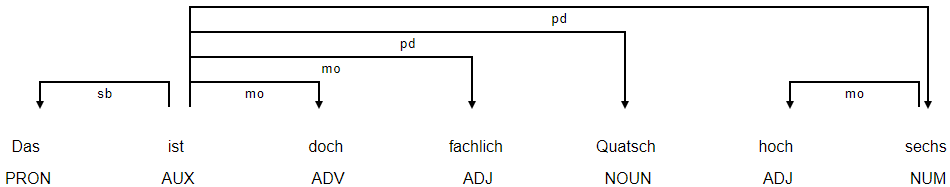
\includegraphics[width=1\textwidth]{chapters/04-Sentiment-Analyse/steffi.png}}
\caption{Visualisierung der Wortabhängigkeiten (Zitat von Steffi Lemke MdB, 208. Sitzung, 10.02.2021)}
\label{steffi}
\end{figure}

\subsection{Negations-Erkennung}
\label{neg-erkennung}
Negation, also Ablehnung, Verneinung oder Aufhebung, hat einen erheblichen Einfluss auf das Ergebnis und damit die Korrektheit der Sentimentanalyse, weshalb in dieser Arbeit ein besonderes Augenmerk auf ihre Erkennung gelegt wurde. 
In \textit{Negation Modeling for German Polarity Classification} \cite{g3_wieg} präsentieren Forscher der Universität des Saarlandes und des Leibniz-Institut für Deutsche Sprache hierfür einen regelbasierten Ansatz. 

Sie definieren unterschiedliche Negationstypen und ihre jeweilige Reichweite. 
So beeinflussen etwa negierende Adverbien oder Indefinitpronomen wie \textit{nie} den gesamten Satz, wohingegen das Partikel \textit{nicht} lediglich seinen Vorgänger negiert.  
Die Tabelle \ref{g3tab1} führt alle in dieser Arbeit implementierten Negationsregeln auf. 
Die Nutzung eines Abhängigkeitsbaumes, wie von \mintinline{latex}{spaCy} ermittelt, ist dabei unerlässlich. 
Denn wie schon im vorherigen Kapitel angesprochen, ist etwa mit dem Vorgänger eines Wortes nicht das in der Satzabfolge voranstehende Wort gemeint, sondern vielmehr der semantische Regent. 

\begin{table}[htbp]
\caption{Implementierte Negations-Regeln aus \cite{g3_wieg}}
\begin{center}
\begin{tabular}{| c | c | c |}
\hline
\textbf{Negationstyp} & \textbf{Reichweite} & \textbf{Beispielworte} \\ \hline
Partikel & Vorgänger (Regent) & nicht \\ \hline
Präpositionen & Nachfolger (Dependent) & ohne, gegen \\ \hline
Adverbien, & Satz & nie, kein, kaum \\
Indefinitpronomen &  &  \\ \hline
Nomen & Genitiv,& Abschaffung, \\
 & Präpositionalobjekt & Zerstörung \\ \hline
Verben & Objekt, Subjekt & enden, sinken, lindern \\
\hline
\end{tabular}
\label{g3tab1}
\end{center}
\end{table}

Angemerkt sei an dieser Stelle, dass es nicht möglich war, alle Regeln aus \cite{g3_wieg} zu implementieren, da der von den Forschern genutzte Dependency-Parser umfangreichere Ergebnisse liefert, als jener von \mintinline{latex}{spaCy}. 

Eine Liste mit Negationsworten und dem jeweiligen Negationstyp wurde \cite{g3_polcla} entnommen und ist ebenfalls über die Klasse \mintinline{latex}{Lexicon} zugreifbar. 
Die Klasse stellt ein \mintinline{latex}{Dictionary} bereit, in welchem die Schlüssel die Negationsworte und die Werte eine Liste der Reichweiten sind. 

Wenn in einem Text ein Negationswort auftritt, werden alle implementierten Regeln geprüft. 
Sollte es zu einem Treffer kommen, etwa wenn das Wort \textit{nicht} auftritt (siehe Abb. \ref{brandner}) und es einen Vorgänger gibt, werden alle Worte in Reichweite des Negationswortes negiert. 
Dies geschieht, indem für die jeweiligen Worte, welche wie in \ref{g3textv} beschrieben \mintinline{latex}{Token}-Objekte sind, ein eigenes Attribut mit der Bezeichnung \mintinline{latex}{negated} auf \mintinline{latex}{True} gesetzt wird. 
In der Polaritätsberechnung wird wortweise auf dieses Attribut geprüft und die Wort-Polarität bei einer Negierung mit -1 multipliziert. 

\begin{figure}[htb]
\centerline{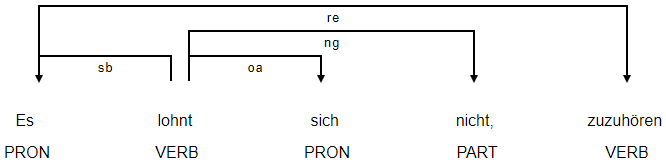
\includegraphics[width=1\textwidth]{chapters/04-Sentiment-Analyse/brandner.png}}
\caption{Beispielsatz mit Patikel-Negation (Zitat von Stephan Brandner MdB, 207. Sitzung, 29.01.2021)}
\label{brandner}
\end{figure}

\subsection{Verstärkungs-Erkennung}
\label{ver-erkennung}
Als \textit{Verstärker} werden sog. Gradpartikel (z.B. sehr, besonders, viel) verstanden, welche direkt vor Adjektiven oder Adverbien in einem Satz auftreten. 
Sie verstärken ihren Nachfolger, was wiederum in der Polaritätsberechnung berücksichtigt werden soll. 

Aus diesem Grund wird eine Liste mit verstärkenden Gradpartikeln, welche ebenfalls aus \cite{g3_polcla} bezogen werden, eingelesen und über die \mintinline{latex}{Lexicon} Klasse bereitgestellt. 

Ebenso wie in Kapitel \ref{neg-erkennung} bereits für die Negation beschrieben, wird ein eigenes Attribut zur Signalisierung einer Verstärkung definiert und im entsprechenden Fall auf True gesetzt. 
Bei der Polaritätsberechnung wird bei einer erkannten Verstärkung die Wort-Polarität mit 1,5 multipliziert \cite{g3_sentia}. 

In Abbildung \ref{hessel} wird ein Beispiel für das Auftreten eines verstärkenden Gradpartikels gegeben. 
Hier verstärkt das Wort \textit{sehr} das negative Wort \textit{spät}, womit die errechnete Polarität stärker negativ ausfällt als ohne die Verstärkungs-Erkennung. 

\begin{figure}[htb]
\centerline{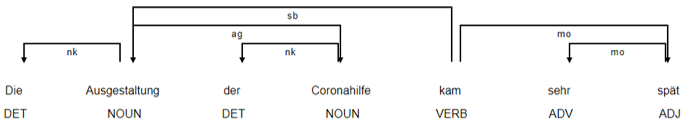
\includegraphics[width=1\textwidth]{chapters/04-Sentiment-Analyse/hessel.png}}
\caption{Beispielsatz mit Gradpartikel-Verstärkung (Zitat von Katja Hessel MdB, 206. Sitzung, 28.01.2021)}
\label{hessel}
\end{figure}

\subsection{Polaritätsberechnung}
\label{polberechnung}
Für die abschließende Berechnung der Polarität sind verschiedene Formeln denkbar. 
Sie sollten anhand von Textcharakteristika wie z.B. der Satz- oder Textlänge gewählt werden. 

Bei der Verwendung einer satzbasierten Polaritätsberechnung, bei welcher alle Polaritäten erst addiert und die Summe anschließend durch die Anzahl der Worte dividiert wird, kann ein unerwünschtes Phänomen auftreten: 
Längere Sätze erhaltenen ein stärker polarisiertes Ergebnis als vergleichbare kurze Sätze. 

Dies ist mit einer im Schnitt höheren Dichte an Worten mit Polaritäts-Wert in längeren Sätzen zu erklären. 
Um diesem Problem entgegen zu wirken, wurde in dieser Arbeit eine Min-Max-Skalierung (siehe Formeln 1 - 3) auf Dokumentebene implementiert \cite{g3_sentia}. 

Die Entscheidung, diese Normalisierung anhand der Länge des gesamten Textes durchzuführen, wurde aufgrund der Charakteristika der zu analysierenden Interaktionen getroffen. 
Denn diese bestehen zu einem überwiegenden Teil aus einem einzelnen Satz von jedoch sehr unterschiedlicher Länge. 

\begin{align}
p' &= \frac{ p + 1 }{ text.len + 1 } \text{ für p $>$ 0}\\
p' &= \frac{ p - 1 }{ text.len + 1 } \text{ für p $<$ 0}\\
p' &= p \text{ für p $=$ 0}
\end{align}

\section{Evaluierung}
\subsection{Sprache im Bundestag}
\label{sprachebundestag}
Während der Entwicklung dieser Arbeit und den regelmäßig angestellten Zwischentests wurde ersichtlich, dass sich die Sprache im Bundestag etwa von jener in sozialen Netzwerken oder Produktbewertungen unterschiedet. 
Ein Interaktionstext setzt sich sowohl aus einzelnen, langen und komplexe Sätze zusammen, als auch aus einzelnen Ausrufen wie \textit{\glqq eieiei!\grqq} zusammen. 

Aus diesem Grund wurde die in \ref{polberechnung} beschriebene Normalisierung verwendet, da herkömmliche Berechnungsformeln zunächst widersprüchliche Ergebnisse lieferten. 
Gleichzeitig verbesserte die manuelle Durchsicht der häufigsten 15.000 Worte und Anfertigung einer eigenen Bundestags-Wortliste das Ergebnis deutlich. 
Viele der regelmäßig in Bundestagssitzungen verwendeten Worte gehören zur \textit{Politik-Domäne} und treten deshalb nicht in den Quell-Wortlisten auf. 
Hier wird erwartet, dass eine noch umfangreichere Bundestags-Wortliste einen weiteren positiven Einfluss auf das Endergebnis hätte. 
Aus Zeit- sowie Kompetenzgründen wurde diese Liste jedoch nicht erweitert. 

\subsection{Ironie und Sarkasmus}
Ebenso wie die im vorherigen besprochene \textit{Politiksprache}, treten auch Ironie und Sarkasmus vermehrt in den Sitzungen des Bundestages auf. 
Einfach umrissen, handelt es sich dabei um ein Stilmittel, bei dem das Gegenteil vom Gesagten gemeint ist. 
Sarkasmus ist dabei eine verstärkte Form der Ironie und kann auch als ein Angriff verstanden werden. 

Selbst für den menschlichen Leser ist allein am geschriebenen Text nicht immer ersichtlich, ob eine Aussage ironisch gemeint ist. 
Vielmehr wird für die richtige Deutung die Stimmlage, Gestik und Mimik der sprechenden Person benötigt. 

Ironie und Sarkasmus könne also erst recht nicht mit dem in dieser Arbeit verwendeten Wortlisten-Ansatz erkannt werden, womit ein unbekannter Teil der Interaktionen im Ergebnis die falsche Polarität besitzt. 
Gleichwohl gibt es Ansätze aus dem Bereich des maschinellen Lernens, welche dieses Problem behandeln. 
Jedoch setzen diese einen entsprechend annotierten Korpus vorraus und stammen zudem aus dem Bereich der sozialen Netzwerke, in welchen etwa mit \textit{Hashtags} die Ironie bereits vom Autor markiert wurde. 

\subsection{Fazit}
Trotzt der soeben beschriebenen Fehlerquellen, wurde dennoch ein gelungenes Ergebnis erzielt: 
Es wurde ein solider und erweiterbarer Algorithmus zur Sentimentananlyse von Texten geschaffen, welcher auf den bekanntesten Bibliotheken und Techniken der Textverarbeitung beruht. 
Dieser kann als Basis für weitere Anstrengungen bei der Sentimentanalyse von politischen Texten dienen. 

Eine Deutung der bisherigen Ergebnisse durch Politikwissenschaftler oder anderweitig in diesem Bereich kompetente Personen wird dabei empfohlen, um die beschriebenen Schwachstellen entsprechend zu behandeln oder neue zu identifizieren. 

Der Programmcode ist zudem vollständig und abgesichert in die Projektpipeline eingebunden. 
Er erweitert seine Ergebnis-Datenbank automatisch um neue Sitzungen und benachrichtigt anschließend nachfolgende Gruppen. 

\section{Aufbau der Lösung}\label{sec:01_02_aufbauLoesung}
Das Projekt zur Entwicklung eines graphbasierten Informationssystem für die Analyse sozialer Interaktionen im Deutschen Bundestag, welches \glqq Sentiments Of Bundestag\grqq{} genannt wurde, besteht, wie bereits erwähnt, aus sieben Teilprojekten. Im folgenden Abschnitt wird grob auf die Thematiken der einzelnen Gruppen eingegangen.

\begin{figure}[H]
    \centering
    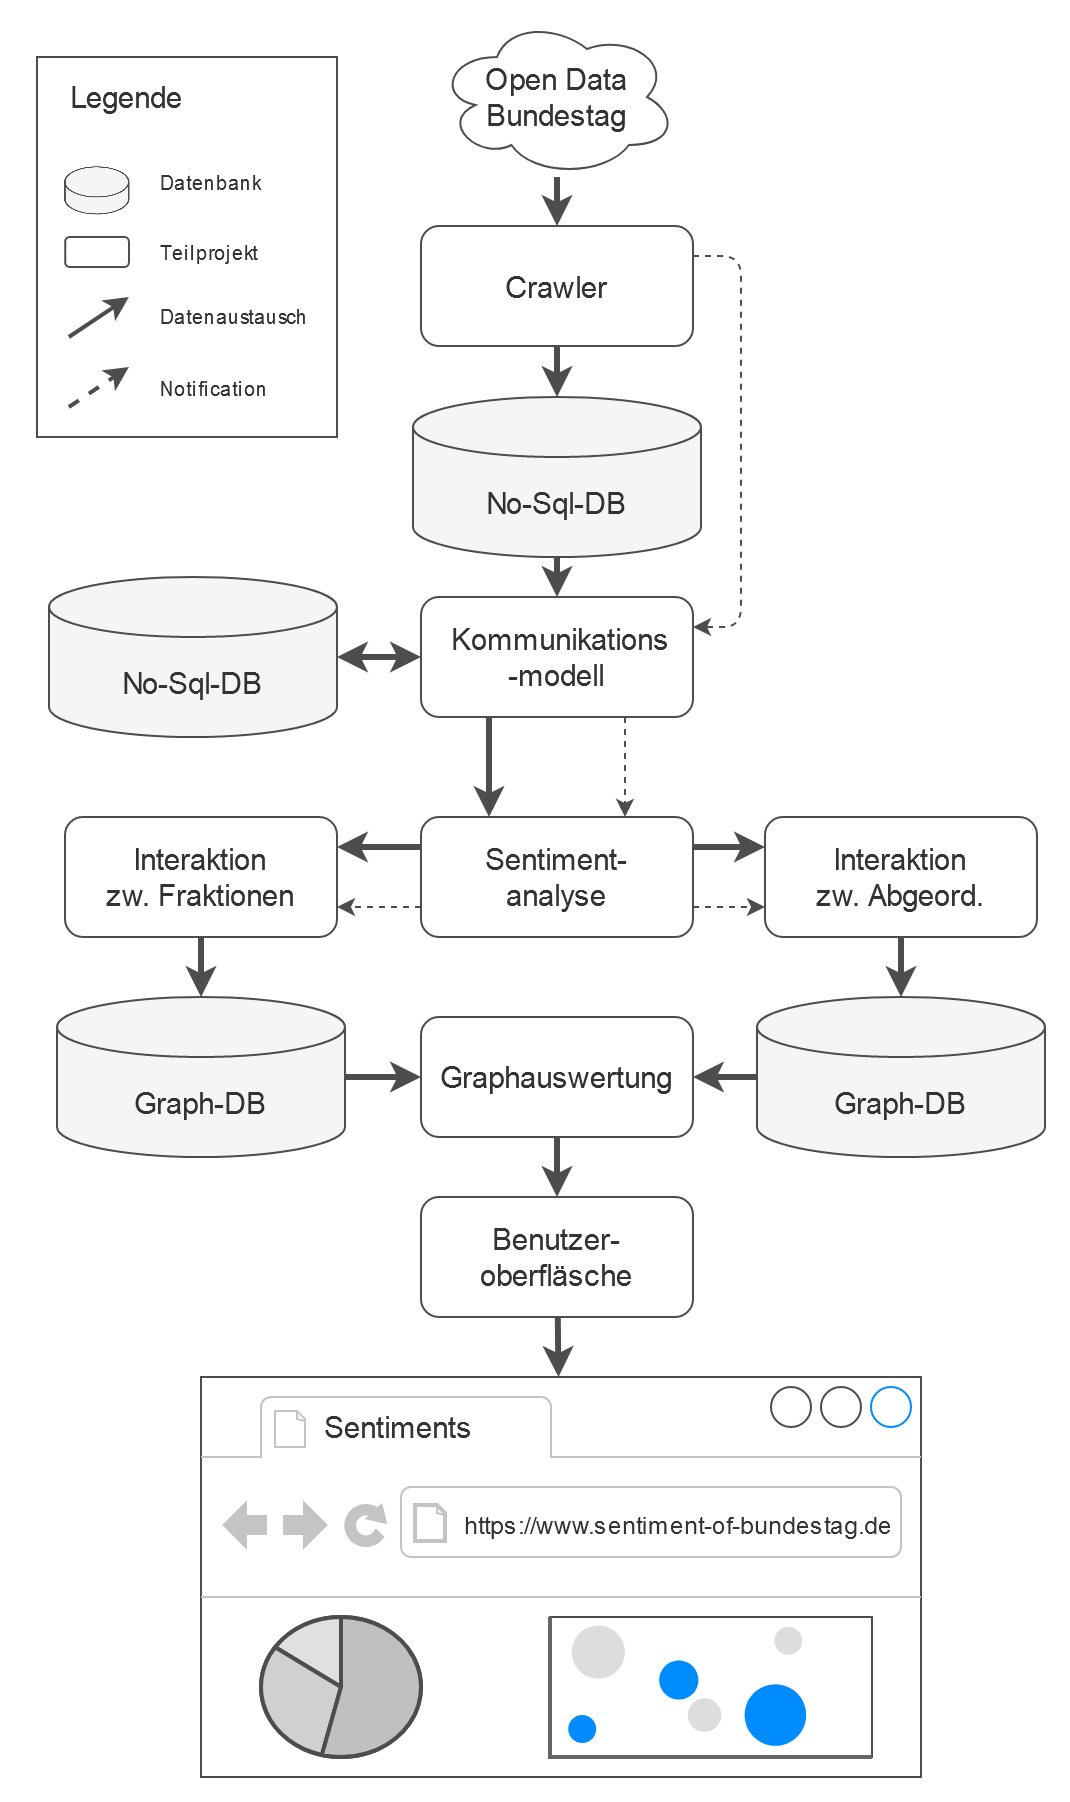
\includegraphics[width=\textwidth]{images/01-Einleitung/SentimentOfBundestag.png}
    \caption{Aufbau der Lösung}
    \label{fig:aufbauderLösungSOB}
\end{figure}

Die in der \autoref{fig:aufbauderLösungSOB} dargestellten Teilprojekte sind hier nun detaillierter aufgelistet:
\begin{itemize}
    \item \textbf{Crawler}: Scannt regelmäßig die Open Data Webseite des Bundestags, sucht, parst und speichern neue Protokollen sowie Stammdaten der Abgeordneten in seiner No-Sql-Datenbank. Ziel ist es hier sicherzustellen, das die DB immer auf dem neusten Stand bleibt
    \item \textbf{Kommunikationsmodell}: Analysiert und erstellt aus den
      Protokollen von Gruppe 1 ein Kommunikationsmodell, welches die möglichen
      Interaktionen im Bundestag abbildet
    \item \textbf{Sentiment-Analyse}: Sentiment Analysis (Stimmungsanalyse). Ziele sind hier die Identifikation der Stimmung in den Äußerungen der Abgeordneten und die Verrechnung der Stimmung einer Äußerung zu positiver/negativer Bewertung der Beziehung
    \item \textbf{Interaktion zwischen Abgeordneten}: Aus dem Kommunikationsmodell von Gruppe 2 und die Stimmungsanalyse von Gruppe 3 werden hier Interaktionen zwischen einzelnen Personen (Abgeordneten, Präsident, Gäste, etc.) identifiziert. Erstellt wird hier ein gewichteter Sentiment-Graph zwischen Abgeordneten mit positiven/negativen Gewichtungen
    \item \textbf{Interaktion zwischen Fraktionen}: Aus dem Kommunikationsmodell von Gruppe 2 und den Sentiment-Graph zwischen Personen von Gruppe 4 werden hier Interaktionen zwischen Gruppen von Personen analysiert und in einen Sentiment-Graph zwischen Parteien. Der besteht aus einer Aggregation der Abgeordnetensentiments zu gewichteten Sentiment-Graph der Parteien (Fraktionen, Gruppen, etc.)
    \item \textbf{Graphauswertung}: Die Sentiment-Graphen von den Gruppen 4 und 5 werden hier anhand verschiedener Auswertungsmethoden analysiert und die Ergebnisse davon die nächste Gruppe (Benutzeroberfläche) zur Verfügung stellt.
    \item \textbf{Benutzeroberfläche}: Ziel ist hier die Realisierung einer interaktiven Benutzeroberfläche zur Darstellung der ausgewerteten Ergebnisse
\end{itemize}

Die einzelnen Teilprojekte werden in den nächsten Kapiteln in dieser Reihenfolge näher erläutert.

\chapter{Crawler}
\thispagestyle{empty}
\begin{table}[ht]
\caption{Gruppe 1 (Crawler) - Arbeitsaufteilung}
\label{tab:zeittafelEU}
\centering
\begin{tabular}{m{12em}|m{12em}|m{8em}}
\hline
\rowcolor{Gray}
Aufgabe &Gruppenmietglieder &Anteil\\
\hline
\hline
\rowcolor{White}
Crawl-Manager& Boris Foko Kouti & ff\\
\hline
\hline
\rowcolor{White}
& Marlon Daniel Kohlberger & ff\\
\cline{2-3}
\rowcolor{White}
\multirow{-2}{*}{Crawl-Utilities}& Boris Foko Kouti & ff\\
\hline
\hline
\rowcolor{White}
& Marlon Daniel Kohlberger & ff\\
\cline{2-3}
\rowcolor{White}
\multirow{-2}{*}{DB-Manager}& Boris Foko Kouti & ff\\
\hline
\hline
\cline{2-3}
\rowcolor{White}
& Arnauld Feussi & ff\\
\rowcolor{White}
& Marlon Daniel Kohlberger & ff\\
\cline{2-3}
\rowcolor{White}
\multirow{-2}{*}{Dokumenation}& Boris Foko Kouti & ff\\
\hline
\hline
\rowcolor{White}
Bereitstellung der Lösung& Boris Foko Kouti & ff\\
\hline
\end{tabular}
\end{table}
\section{Einleitung}
Der Begriff \textit{Sentiment} stammt vom lateinischen Wort \textit{sentimentum} ab und bedeutet Empfindung oder Stimmung. 
In der Sentimentanalyse geht es um die Bestimmung eben jener Stimmung einer Meinungsäußerung. 
Anwendung findet sie etwa bei Produktbewertungen oder Beiträgen in sozialen Netzwerken. 
Die Stimmung wird durch die sog. Polarität beschrieben und kann positiv, negativ oder neutral ausfallen. 
Im Text-Mining wird sie im Intervall $\interval{-1}{1} = \{x \in \mathbb{R} | -1 \leq x \leq 1\}$ angegeben, wobei -1 sehr negativ, 1 sehr positiv und 0 neutral bedeuten. 

Grundlegend ist die maschinelle Sentimentanalyse entweder Wortlisten- oder Modell-basiert. 
Der Wortlisten-Ansatz kann als eine Sammlung von Worten und ihrer Polaritäten verstanden werden, anhand welcher die Stimmung berechnet wird. 
Dieser Ansatz wird weiter im Kapitel \ref{wortliste} beschrieben, da er in dieser Arbeit verwendet wurde. 

Bei der Modell-basierten Sentimentanalyse wird ein annotierter Satz-Korpus für das Trainieren einer künstlichen Intelligenz vorausgesetzt. 
Etwa für Twitter-Beiträge stehen solche Korpusse oder auch bereits trainierte Modelle zur Verfügung. 
Jedoch ist bei der Verwendung zur Analyse der Sitzungsprotokolle des Bundestages nicht mit zufriedenstellenden Ergebnissen zu rechnen, da sich verwendete Worte und Text- bzw. Satzbau zwischen diesen Domänen deutlich unterscheiden. 
Eine weitere Erläuterung zur Sprache im Bundestag wird in Kapitel \ref{sprachebundestag} gegeben. 

Ebenfalls werden die Komponenten zur Teilnahme an der Verarbeitungspipeline des Gesamtprojektes im nachfolgenden Kapitel \ref{g3daten} beschrieben. 

\section{Datenaustausch}
\label{g3daten}
\subsection{Datenimport}
Für das Erhalten von Daten wurde eine Methode implementiert, welche durch Angabe einer Sitzungs-ID die entsprechende Sitzung vom REST-API von Gruppe 2 abfragen kann. 
Diese Methode gibt jede Sitzung weiter an die in Kapitel \ref{g3textv} beschriebene Textverarbeitung und das Ergebnis schließlich an den in Kapitel \ref{g3export} beschriebenen Export-Code. 

Die Methode wird für zwei Fälle verwendet: 
Beim Normalfall sendet die Gruppe 2 eine Benachrichtigung mit einer Liste aller neuen Sitzungs-IDs an das REST-API im Code dieser Arbeit. 
Das REST-API wurde mit der Bibliothek \mintinline{latex}{Flask} \cite{g3_flask} entwickelt und besteht aus einer POST-Schnittstelle, welche auf dem von der HTW bereitgestelltem Server unter \textit{/notify} erreichbar ist. 

Das API wurde unter Zuhilfenahme von \mintinline{latex}{Flask.Blueprints} \cite{g3_flaskbp} entwickelt und wird von einem \mintinline{latex}{Waitress}-Webserver \cite{g3_waitress} bereitgestellt. 
Für jede Anfrage wird geprüft, ob Content-Type und Payload dem erwarteten JSON-Daten entsprechen. 
Sollte dies nicht der Fall sein, wird eine entsprechende Rückmeldung an den Sender zurückgegeben. 
Für jede erhaltene Sitzungs-ID wird die eingangs beschriebene Methode aufgerufen. 

Der zweite Fall wurde vor allem im Rahmen der voranschreitenden Entwicklung bei den in der Projektpipeline voranstehenden Gruppen verwendet. 
Statt auf eine Benachrichtigung zum Anstoßen des Datenimports zu warten, werden stattdessen alle Sitzungs-IDs vom REST-API der Gruppe 2 abgefragt und jede Sitzung vollständig neu importiert. 
Dieses Vorgehen hat den Vorteil, dass eventuell durch Arbeit am Code verpasste Benachrichtigungen nachgeholt werden und gleichzeitig Änderungen an den Daten übernommen werden können. 

\subsection{Datenexport}
\label{g3export}
Statt Arbeit in ein umfangreiches REST-API für die nachfolgenden Gruppen zu stecken, wurde für diese Arbeit ein reiner MongoDB-Ansatz verwendet. 
Auf dem zur Verfügung stehenden HTW-Server wurde dafür eine MongoDB Instanz aufgesetzt, welche nur aus dem HTW-Netz erreichbar und zudem nur mit Authentifizierung zugreifbar ist. 
Jede Sitzung ist hier als eine eigene Collection persistiert. 
Sobald neue Sitzungen importiert und verarbeitet wurden, werden diese zunächst mit dem MongoDB-Treiber \mintinline{latex}{PyMongo} \cite{g3_mongodb} in die Datenbank geschrieben. 
Anschließend werden die nachfolgenden Gruppen mit einem POST and die jeweilige REST-Schnittstelle benachrichtigt, dass neue Daten vorliegen. 
Diese greifen dann mit den zuvor versendeten Zugangsdaten direkt auf die Datenbank zu. 

Mit diesem Vorgehen konnte die Komplexität beim Zugriff auf die Ergebnis-Daten gesenkt werden, da es für nahezu alle gängigen Programmiersprachen einen intuitiven MongoDB-Treiber gibt. 

\section{Wortliste}
\label{wortliste}
Wie bereits in der Einleitung beschrieben, handelt es sich bei Wortlisten in der Sentimentanalyse um eine Liste von Worten und ihrer jeweiligen Polarität. 
Bei der Analyse eines Textes wird wortweise ein Abgleich mit dieser Liste durchgeführt und die Wort-Polarität bei einer Übereinstimmung für die Berechnung des Sentiments verwendet. 
Unterschiedliche Berechnungsformeln sind dabei denkbar und werden in Kapitel \ref{polberechnung} weiter besprochen. 
Für diese Arbeit wurden Wortlisten verschiedener Institutionen kombiniert und anschließend mit Synonymen erweitert. 
Ebenfalls wurde eine eigene Bundestags-Wortliste erstellt. 

Die Interest Group on German Sentiment Analysis (IGGSA) stellt eine umfangreiche Liste an Publikationen und Ressourcen zu Sentimentanalysen in der deutschen Sprache zur Verfügung \cite{g3_iggsa}. 
Hier wurden alle Referenzen auf die in dieser Arbeit verwendeten Quell-Wortlisten gesammelt. 
Für die Zusammenführung dieser Wortlisten wurden zunächst zwei Herangehensweisen evaluiert: 
Zum einen war die Erstellung eines eigenständigen Codes denkbar, welcher einmalig die Daten aus allen Quellen einliest, zusammenfasst und eine Ergebnis-Datei ausgibt. 
Diese Datei wäre eine Ressource für den eigentlichen Analyse-Code. 
Zum anderen könnte die soeben beschriebene Funktionalität jedoch auch direkt im Analyse-Code integriert und bei jedem Programmstart ausgeführt werden. 
Die kombinierte Wortliste würde somit nicht auf die Festplatte geschrieben, sondern im Arbeitsspeicher verbleiben, solange der Analyse-Code läuft. 
Wenngleich der zuerst beschriebene Ansatz offensichtlich weniger Rechenzeitaufwändig ist, wurde für diese Arbeit der zweite Ansatz gewählt. 
Dies wird vor allem mit Rechtsunsicherheiten bei der Arbeit mit den verschiedenen Lizenzen der Quelldateien begründet. 
Gleichzeitig arbeitet der Analyse-Code damit jederzeit mit dem aktuellen Stand der Quell-Wortlisten. 
Das Aufbauen der Wortliste dauert wenige Minuten. 

Für diese Arbeit wurden die folgenden Quell-Wortlisten verwendet: 

\begin{itemize}
\item \textit{SentimentWortschatz} (SentiWS) aus \glqq SentiWS - a Publicly Available German-language Resource for Sentiment Analysis\grqq (Universität Leipzig) \cite{g3_sentiws}
\item \textit{Multi-Domain Sentiment Lexicon for German} (Hochschule Darmstadt) \cite{g3_opm}
\item \textit{German Polarity Lexicon} aus \glqq Evaluation and extension of a polarity lexicon for German\grqq (Universität Zürich) \cite{g3_polcla}
\item \textit{morphcomp} aus \glqq Evaluating the morphological compositionality of pola-rity\grqq (Leibniz-Institut für Deutsche Sprache, Universität des Saarlandes) \cite{g3_morphcomp}
\end{itemize}

Aus diesen Quellen ergibt sich eine Wortliste mit etwa 14.000 einzigartigen Worten. 
Die Worte werden dabei mit der in Kapitel \ref{g3textv} beschriebenen Textverarbeitungspipeline lemmatisiert, also auf die Grundform zurückgeführt. 
Bei Überschneidungen wird ein Mittelwert über alle Polaritäts-Werte eines Wortes gebildet. 

Mithilfe des \textit{Open German WordNet} (OdeNet) \cite{g3_odenet} werden zu jedem Wort Synonyme gesammelt und ebenfalls der Wortliste hinzugefügt. 
Der Zugriff auf OdeNet geschieht dabei mit der python Bibliothek \mintinline{latex}{WN} \cite{g3_wn}. 
Die Verwendung dieser Bibliothek ist trivial, weshalb an dieser Stelle keine weitere Erläuterung gegeben wird. 
Die Wortliste wird durch das Hinzufügen von Synonymen um weitere rund 2.000 Worte erweitert. 

Wie bereits in der Einleitung erwähnt, wurde zudem eine eigene Bundes-tags-Wortliste erstellt. 
Hierzu wurden die 15.000 am häufigsten in den Sitzungsprotokollen vorkommenden Worte erfasst und analysiert. 
Dabei wurden jedoch nur jene Worte betrachtet, welche nicht bereits in der kombinierten Wortliste vorkommen. 
Ausgewählt wurden nur eindeutig positive oder negative Worte wie \textit{angemessen}, \textit{Bullshit}, \textit{Fehlentscheidung}, \textit{Milchmädchenrechnung}, \textit{Realitätsverweigerung}, \textit{Totalausfall} oder \textit{Verunglimpfung}. 
Insgesamt umfasst die Bundestags-Wortliste 217 Worte. 

Im Code wird der Zugriff auf die Wortliste mit der zentralen Klasse \mintinline{latex}{Lexicon} realisiert. 
Bei der Instanziierung der Klasse werden, wie im Vorherigen beschrieben, alle Wortlisten gesammelt, zusammengeführt und erweitert. 
Anschließend stellt die Klasse ein \mintinline{latex}{Dictionary} bereit, in welchem die Schlüssel die Worte und die Werte die Wort-Polarität angeben. 

\section{Textverarbeitung}
\label{g3textv}
Für die Textverarbeitung nutzt der Code dieser Arbeit vollständig die Funktionalitäten und Strukturen von \mintinline{latex}{spaCy} \cite{g3_spacy}. 
Die \mintinline{latex}{spaCy} Bibliothek stellt eine Textverarbeitungspipeline bereit, welche mithilfe eines vortrainierten Modells funktioniert. 
Für die deutsche Sprache wurde ein solches Modell mit dem TIGER Korpus der Universität Stuttgart trainiert. 
Der Korpus umfasst ca. 50.000 Sätze aus Texten der Frankfurter Rundschau. 
Die \mintinline{latex}{spaCy}-Pipeline besteht aus den folgenden Komponenten: 

\begin{itemize}
\item Tokenisierung (Text- und Satzzerteilung)
\item POS-Tagging (Wortartenerkennung)
\item Dependency-Parsing (Wortabhängigkeitenerkennung)
\item Lemmatisierung (Wortgrundformermittlung)
\item Entity-Recognition (Eigennamenerkennung)
\end{itemize}

Das Ergebnis der Pipeline ist ein \mintinline{latex}{Doc}-Objekt, welches das Ergebnis des gesamten in die Pipeline gegebenen Textes umfasst. 
Einzelne Sätze innerhalb des \mintinline{latex}{Doc}-Objektes werden mit \mintinline{latex}{Span}-Objekten beschrieben und einzelne Worte mit \mintinline{latex}{Token}-Objekten. 
Die Objekttypen besitzen jeweils eigene Methoden und Erweiterungsmöglichkeiten in Form von sog. \textit{extension attributes}. 

Sehr einfach und gleichzeitig umfangreich kann die \mintinline{latex}{spaCy}-Pipeline an die eigenen Bedürfnisse angepasst werden. 
So wurde die Berechnung des Sentiments eines Textes direkt an die Komponenten der Standart-Pipeline angehängt. 
Logisch unterteilt sich diese in die Komponenten:

\begin{itemize}
\item Negations-Erkennung (siehe \ref{neg-erkennung})
\item Verstärkungs-Erkennung (siehe \ref{ver-erkennung})
\item Polaritätsberechnung (siehe \ref{polberechnung})
\end{itemize}

Basis für das nachfolgende Kapitel \ref{neg-erkennung} ist dabei das Ergebnis des Depen-dency-Parsers von \mintinline{latex}{spaCy}. 
Dieser bestimmt die Abhängigkeiten zwischen den einzelnen Elementen eines Satzes. 
Diese Funktion gehört dem Themenbereich der Dependenzgrammatik an, in welcher gerichtete Beziehungen zwischen den Worten eines Satzes beschreibt werden. 
Ein Wort kann einen Vorgänger (Regent) und mehrere Nachfolger (Dependenten) besitzen. 
Die Gesamtheit der Beziehungen eines Satzes wird auch Abhängigkeitsbaum genannt. 

Zur Verdeutlichung soll die Abbildung \ref{steffi} dienen, welche mithilfe von \mintinline{latex}{spaCy.displaCy} erstellt wurde. 
Zu sehen ist hier der Abhängigkeitsbaum des Satzes \textit{\glqq Das ist doch fachlich Quatsch hoch sechs!\grqq}. 
An den gerichteten Kanten befindet sich die Angabe des Satzgliedes, unterhalb der Worte die Angabe der Wortart. 

\begin{figure}[htb]
\centerline{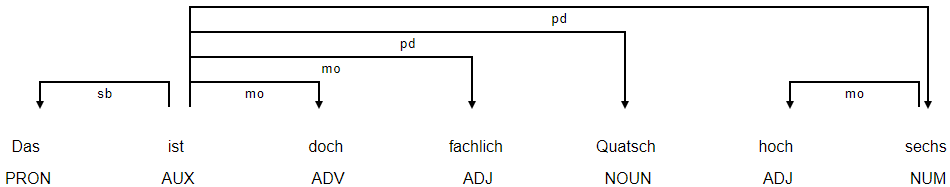
\includegraphics[width=1\textwidth]{chapters/04-Sentiment-Analyse/steffi.png}}
\caption{Visualisierung der Wortabhängigkeiten (Zitat von Steffi Lemke MdB, 208. Sitzung, 10.02.2021)}
\label{steffi}
\end{figure}

\subsection{Negations-Erkennung}
\label{neg-erkennung}
Negation, also Ablehnung, Verneinung oder Aufhebung, hat einen erheblichen Einfluss auf das Ergebnis und damit die Korrektheit der Sentimentanalyse, weshalb in dieser Arbeit ein besonderes Augenmerk auf ihre Erkennung gelegt wurde. 
In \textit{Negation Modeling for German Polarity Classification} \cite{g3_wieg} präsentieren Forscher der Universität des Saarlandes und des Leibniz-Institut für Deutsche Sprache hierfür einen regelbasierten Ansatz. 

Sie definieren unterschiedliche Negationstypen und ihre jeweilige Reichweite. 
So beeinflussen etwa negierende Adverbien oder Indefinitpronomen wie \textit{nie} den gesamten Satz, wohingegen das Partikel \textit{nicht} lediglich seinen Vorgänger negiert.  
Die Tabelle \ref{g3tab1} führt alle in dieser Arbeit implementierten Negationsregeln auf. 
Die Nutzung eines Abhängigkeitsbaumes, wie von \mintinline{latex}{spaCy} ermittelt, ist dabei unerlässlich. 
Denn wie schon im vorherigen Kapitel angesprochen, ist etwa mit dem Vorgänger eines Wortes nicht das in der Satzabfolge voranstehende Wort gemeint, sondern vielmehr der semantische Regent. 

\begin{table}[htbp]
\caption{Implementierte Negations-Regeln aus \cite{g3_wieg}}
\begin{center}
\begin{tabular}{| c | c | c |}
\hline
\textbf{Negationstyp} & \textbf{Reichweite} & \textbf{Beispielworte} \\ \hline
Partikel & Vorgänger (Regent) & nicht \\ \hline
Präpositionen & Nachfolger (Dependent) & ohne, gegen \\ \hline
Adverbien, & Satz & nie, kein, kaum \\
Indefinitpronomen &  &  \\ \hline
Nomen & Genitiv,& Abschaffung, \\
 & Präpositionalobjekt & Zerstörung \\ \hline
Verben & Objekt, Subjekt & enden, sinken, lindern \\
\hline
\end{tabular}
\label{g3tab1}
\end{center}
\end{table}

Angemerkt sei an dieser Stelle, dass es nicht möglich war, alle Regeln aus \cite{g3_wieg} zu implementieren, da der von den Forschern genutzte Dependency-Parser umfangreichere Ergebnisse liefert, als jener von \mintinline{latex}{spaCy}. 

Eine Liste mit Negationsworten und dem jeweiligen Negationstyp wurde \cite{g3_polcla} entnommen und ist ebenfalls über die Klasse \mintinline{latex}{Lexicon} zugreifbar. 
Die Klasse stellt ein \mintinline{latex}{Dictionary} bereit, in welchem die Schlüssel die Negationsworte und die Werte eine Liste der Reichweiten sind. 

Wenn in einem Text ein Negationswort auftritt, werden alle implementierten Regeln geprüft. 
Sollte es zu einem Treffer kommen, etwa wenn das Wort \textit{nicht} auftritt (siehe Abb. \ref{brandner}) und es einen Vorgänger gibt, werden alle Worte in Reichweite des Negationswortes negiert. 
Dies geschieht, indem für die jeweiligen Worte, welche wie in \ref{g3textv} beschrieben \mintinline{latex}{Token}-Objekte sind, ein eigenes Attribut mit der Bezeichnung \mintinline{latex}{negated} auf \mintinline{latex}{True} gesetzt wird. 
In der Polaritätsberechnung wird wortweise auf dieses Attribut geprüft und die Wort-Polarität bei einer Negierung mit -1 multipliziert. 

\begin{figure}[htb]
\centerline{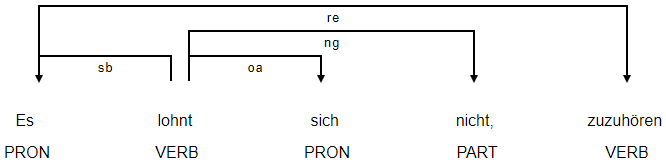
\includegraphics[width=1\textwidth]{chapters/04-Sentiment-Analyse/brandner.png}}
\caption{Beispielsatz mit Patikel-Negation (Zitat von Stephan Brandner MdB, 207. Sitzung, 29.01.2021)}
\label{brandner}
\end{figure}

\subsection{Verstärkungs-Erkennung}
\label{ver-erkennung}
Als \textit{Verstärker} werden sog. Gradpartikel (z.B. sehr, besonders, viel) verstanden, welche direkt vor Adjektiven oder Adverbien in einem Satz auftreten. 
Sie verstärken ihren Nachfolger, was wiederum in der Polaritätsberechnung berücksichtigt werden soll. 

Aus diesem Grund wird eine Liste mit verstärkenden Gradpartikeln, welche ebenfalls aus \cite{g3_polcla} bezogen werden, eingelesen und über die \mintinline{latex}{Lexicon} Klasse bereitgestellt. 

Ebenso wie in Kapitel \ref{neg-erkennung} bereits für die Negation beschrieben, wird ein eigenes Attribut zur Signalisierung einer Verstärkung definiert und im entsprechenden Fall auf True gesetzt. 
Bei der Polaritätsberechnung wird bei einer erkannten Verstärkung die Wort-Polarität mit 1,5 multipliziert \cite{g3_sentia}. 

In Abbildung \ref{hessel} wird ein Beispiel für das Auftreten eines verstärkenden Gradpartikels gegeben. 
Hier verstärkt das Wort \textit{sehr} das negative Wort \textit{spät}, womit die errechnete Polarität stärker negativ ausfällt als ohne die Verstärkungs-Erkennung. 

\begin{figure}[htb]
\centerline{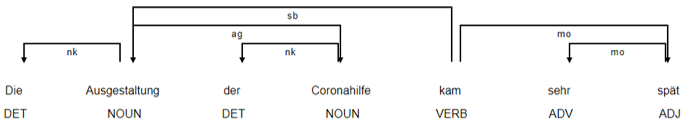
\includegraphics[width=1\textwidth]{chapters/04-Sentiment-Analyse/hessel.png}}
\caption{Beispielsatz mit Gradpartikel-Verstärkung (Zitat von Katja Hessel MdB, 206. Sitzung, 28.01.2021)}
\label{hessel}
\end{figure}

\subsection{Polaritätsberechnung}
\label{polberechnung}
Für die abschließende Berechnung der Polarität sind verschiedene Formeln denkbar. 
Sie sollten anhand von Textcharakteristika wie z.B. der Satz- oder Textlänge gewählt werden. 

Bei der Verwendung einer satzbasierten Polaritätsberechnung, bei welcher alle Polaritäten erst addiert und die Summe anschließend durch die Anzahl der Worte dividiert wird, kann ein unerwünschtes Phänomen auftreten: 
Längere Sätze erhaltenen ein stärker polarisiertes Ergebnis als vergleichbare kurze Sätze. 

Dies ist mit einer im Schnitt höheren Dichte an Worten mit Polaritäts-Wert in längeren Sätzen zu erklären. 
Um diesem Problem entgegen zu wirken, wurde in dieser Arbeit eine Min-Max-Skalierung (siehe Formeln 1 - 3) auf Dokumentebene implementiert \cite{g3_sentia}. 

Die Entscheidung, diese Normalisierung anhand der Länge des gesamten Textes durchzuführen, wurde aufgrund der Charakteristika der zu analysierenden Interaktionen getroffen. 
Denn diese bestehen zu einem überwiegenden Teil aus einem einzelnen Satz von jedoch sehr unterschiedlicher Länge. 

\begin{align}
p' &= \frac{ p + 1 }{ text.len + 1 } \text{ für p $>$ 0}\\
p' &= \frac{ p - 1 }{ text.len + 1 } \text{ für p $<$ 0}\\
p' &= p \text{ für p $=$ 0}
\end{align}

\section{Evaluierung}
\subsection{Sprache im Bundestag}
\label{sprachebundestag}
Während der Entwicklung dieser Arbeit und den regelmäßig angestellten Zwischentests wurde ersichtlich, dass sich die Sprache im Bundestag etwa von jener in sozialen Netzwerken oder Produktbewertungen unterschiedet. 
Ein Interaktionstext setzt sich sowohl aus einzelnen, langen und komplexe Sätze zusammen, als auch aus einzelnen Ausrufen wie \textit{\glqq eieiei!\grqq} zusammen. 

Aus diesem Grund wurde die in \ref{polberechnung} beschriebene Normalisierung verwendet, da herkömmliche Berechnungsformeln zunächst widersprüchliche Ergebnisse lieferten. 
Gleichzeitig verbesserte die manuelle Durchsicht der häufigsten 15.000 Worte und Anfertigung einer eigenen Bundestags-Wortliste das Ergebnis deutlich. 
Viele der regelmäßig in Bundestagssitzungen verwendeten Worte gehören zur \textit{Politik-Domäne} und treten deshalb nicht in den Quell-Wortlisten auf. 
Hier wird erwartet, dass eine noch umfangreichere Bundestags-Wortliste einen weiteren positiven Einfluss auf das Endergebnis hätte. 
Aus Zeit- sowie Kompetenzgründen wurde diese Liste jedoch nicht erweitert. 

\subsection{Ironie und Sarkasmus}
Ebenso wie die im vorherigen besprochene \textit{Politiksprache}, treten auch Ironie und Sarkasmus vermehrt in den Sitzungen des Bundestages auf. 
Einfach umrissen, handelt es sich dabei um ein Stilmittel, bei dem das Gegenteil vom Gesagten gemeint ist. 
Sarkasmus ist dabei eine verstärkte Form der Ironie und kann auch als ein Angriff verstanden werden. 

Selbst für den menschlichen Leser ist allein am geschriebenen Text nicht immer ersichtlich, ob eine Aussage ironisch gemeint ist. 
Vielmehr wird für die richtige Deutung die Stimmlage, Gestik und Mimik der sprechenden Person benötigt. 

Ironie und Sarkasmus könne also erst recht nicht mit dem in dieser Arbeit verwendeten Wortlisten-Ansatz erkannt werden, womit ein unbekannter Teil der Interaktionen im Ergebnis die falsche Polarität besitzt. 
Gleichwohl gibt es Ansätze aus dem Bereich des maschinellen Lernens, welche dieses Problem behandeln. 
Jedoch setzen diese einen entsprechend annotierten Korpus vorraus und stammen zudem aus dem Bereich der sozialen Netzwerke, in welchen etwa mit \textit{Hashtags} die Ironie bereits vom Autor markiert wurde. 

\subsection{Fazit}
Trotzt der soeben beschriebenen Fehlerquellen, wurde dennoch ein gelungenes Ergebnis erzielt: 
Es wurde ein solider und erweiterbarer Algorithmus zur Sentimentananlyse von Texten geschaffen, welcher auf den bekanntesten Bibliotheken und Techniken der Textverarbeitung beruht. 
Dieser kann als Basis für weitere Anstrengungen bei der Sentimentanalyse von politischen Texten dienen. 

Eine Deutung der bisherigen Ergebnisse durch Politikwissenschaftler oder anderweitig in diesem Bereich kompetente Personen wird dabei empfohlen, um die beschriebenen Schwachstellen entsprechend zu behandeln oder neue zu identifizieren. 

Der Programmcode ist zudem vollständig und abgesichert in die Projektpipeline eingebunden. 
Er erweitert seine Ergebnis-Datenbank automatisch um neue Sitzungen und benachrichtigt anschließend nachfolgende Gruppen. 

\section{Anforderungen und Rahmenbedingungen}\label{sec:02_02_anforderungen_rahmen}
Der zu entwickelnden Crawler soll in bestimmten Rahmenbedingungen einige Anforderungen erfüllen. Diese sowie die technischen und organisatorischen Rahmenbedingungen dazu werden in diesem Abschnitt aufgelistet. 
\subsection{Anforderungen an dem Crawler}\label{subsec:02_02_anforderungen}
Die Anforderungen an dem Crawler sind in~\cite{Hoppe2020Uebung} zusammengefasst und sehen vor, dass der Crawler kontinuierlich laufen sollte und dabei nach folgenden Dateien suchen:
\begin{itemize}
  \item \textbf{Protokolle}: Ein Protokoll ist eine XML-Datei, die den gesamten Ablauf einer Plenarsitzung (Inhaltsverzeichnis, Sitzungsverlauf mit Sitzungsbeginn, Tagesordnungspunkte, Sitzungsende, Anlagen, Rednerliste und  gewisse Konfigs) beinhaltet. Da sich die Formatierung der Protokollen in den Jahren stets verbessert hat, soll hier auf die Legislaturperioden geachtet werden:
  \begin{itemize}
    \item 19. Legislaturperiode: diese sind sehr gut strukturiert und leicht zu parsen
    \item 18. Legislaturperiode: schlechter formatiert als die 19. Legislaturperiode. Hierfür wird vom Prof. Dr. Thomas Hoppe eine mit besser formatierte Version zur Verfügung gestellt
  \end{itemize}
  \item \textbf{Stammdaten der Abgeordneten}: Ist eine XML-Datei, die Informationen über Abgeordneten seit 1949 sammelt
  \item \textit{Optional} \textbf{Namentliche Abstimmungen}: Liste aller namentlichen Abstimmungen im Bundestag seit dem 18.12.2009 in PDF-Format und seit dem 18.10.2012 auch in XLSX-Format~\cite{NamentlicheAbstimmung20}
  \item Es muss sichergestellt sein, dass alle Daten immer auf dem neusten Stand sind. Dafür soll die Frequenz des Crawlers sich an dem Sitzungskalender des Bundestags~\cite{Sitzungskalender2021} orientieren
\end{itemize}

\subsection{Rahmenbedingungen}\label{subsec:02_02_rahmenbedingungen}
\subsubsection{Organisatorische Rahmenbedingungen}
Für die Planung des gesamten Projekts ist in einem zwei Wochen-Takt ein Plenum für den Brainstorming und eventuelle Teams-übergreifende Abstimmungen festgelegt worden. Im Team-Crawler (Gruppe 1) ist folgende Planung abgemacht worden:
\begin{itemize}
    \item Ziel bis zum 13.11.2020: Testdaten für andere Gruppen, erster lauffähiger Prototyp
    \item Ziel bis zum 27.11.2020: Vorläufiger Release und Integration-Test mit anderen Gruppen (Kommunikationsmodell)
    \item Ziel bis zum 04.12.2020: finale Version und Anfang der Dokumentation
    \item Ziel bis zum 25.02.2021: Fertigstellung der Dokumentation und Abgabe
\end{itemize}
Neben den organisatorischen Rahmenbedingungen sind technische Rahmenbedingungen zu betrachten bzw. sind Fehler (Probleme) zu vermeiden (zu lösen).
\subsubsection{Technische Rahmenbedingungen: Probleme beim Crawlen}\label{subsubsec:techAnforderungen}
\begin{itemize}
    \item Sperrung durch Server-Administrator (Server-Regel). Es soll vermieden werden, dass der ausführende Rechner wegen zu häufige Abfragen vom Server-Admin gesperrt wird und nur noch ein 500-Fehlercode erhält
    \item Ajax basierende Inhalte. Die Open Data Webseite verwendet Ajax für die Bereitstellung der Daten und lädt diese im Hintergrund. Ein einfacher Download der Seite genug da nicht. Außerdem nutzen die meisten Links, hinter denen Dateien stehen, Javascript (es ist z. B. der Fall bei Slides und verborgenen Regionen). Dies muss entsprechend gehandelt werden
    \item Mongo-DB-Konfiguration und Zurverfügungstellung der Daten für die Gruppe Kommunikationsmodell 
    %\item Das robots.txt Protokoll
\end{itemize}
\section{Lösung und Konzepte}\label{sec:02_03_loesung_konzept}
\subsection{Standard Aufbau eines Crawlers}
\begin{wrapfigure}{R}{0.4\textwidth}
  \centering
    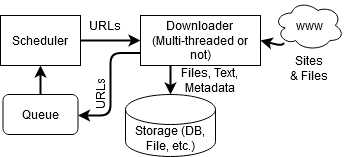
\includegraphics[width=0.4\textwidth]{images/02-Crawler/Crawler-Standard-Crawler.png}
  \caption{\label{fig:standardCrawler}Crawler: Standard Aufbau}
\end{wrapfigure}
Ein Crawler besteht in der Regel aus zwei wichtigen Teilen: ein Downloader und ein Scheduler. Der Downloader ist mit dem Webserver verbunden und lädt die Webseite(n) sowie alle erwünschten Dateien herunter. Der Scheduler ist, wie der Name schon sagt, für die Planung zuständig und erteilt dem Downloader URLs nach internen Priorisierung-Mechanismen (als Liste FIFO und als Graph mit DFS und BFS ~\cite{ThomasAlgorithms2009}--\cite{DonaldKnuth1998}). 
\subsection{Crawler Mechanismus}
Für unseren speziellen Fall, wird die Aufgaben von dem Scheduler vom Crawl-Manager übernommen, der sowohl für die Planung als auch für die Steuerung (Start, Pause, Stopp, Zustand) laufender Crawl-Aufgaben zuständig ist. Der Crawl-Manager erzeugt für jede URL ein Thread (Page-Crawler), dessen Aufgabe darin besteht die Seite herunterzuladen, mit seinem Page-Analyser nach relevanten Inhalten in der Seite zu suchen (URLs, Dateien, Action-Links: Javascript, etc.) und bei Bedarf weitere parallele Sub-Threads für den Download, das Parsen und die Speicherung der relevanten Dateiinhalte (Protokollen, Stammdaten, weitere Metadaten). Dieser Mechanismus wird durch die Abb.~\ref{fig:funktionsprinzipCrawler} und die Abb.~\ref{fig:crawlEinerUrl} veranschaulicht.

\begin{figure}[H]
    \centering
    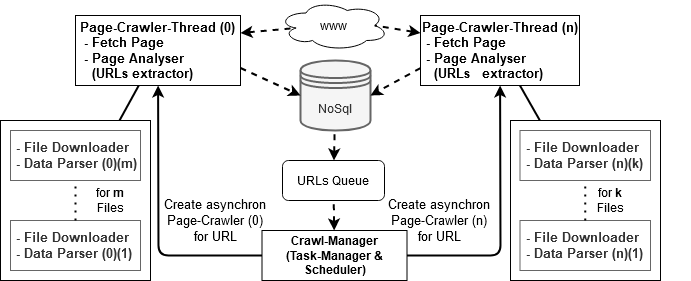
\includegraphics[width=5in]{images/02-Crawler/Crawler-Process-Diagram (Multithreading).png}
    \caption{Funktionsprinzip des unseres Crawlers}
    \label{fig:funktionsprinzipCrawler}
\end{figure}

\begin{figure}[H]
    \centering
    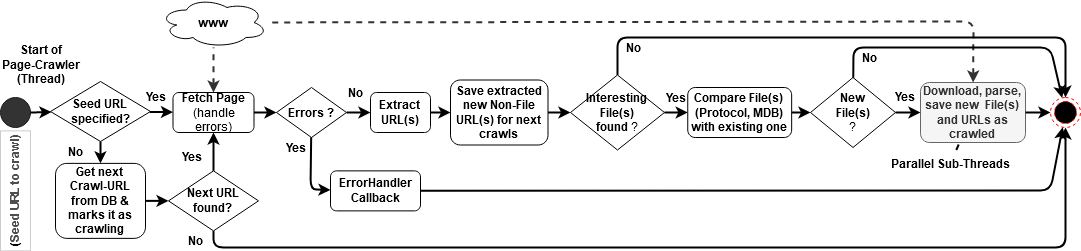
\includegraphics[width=5.5in]{images/02-Crawler/Crawler-Process-Diagram (Page-Crawler).png}
    \caption{Page-Crawler für eine URL}
    \label{fig:crawlEinerUrl}
\end{figure}
\noindent
Ein Crawl auf einer Seite (durch den Page-Crawl) kann in einer durch den Scheduler (Crawl-Manager) regelmäßig gemacht werden, in dem dieser nach einer bestimmten Zeit einen neuen Page-Crawl-Thread startet. Die Frequenz der Generierung dieses Threads orientiert sich an dem Sitzungskalender des Bundestags~\cite{Sitzungskalender2021}. Dieser Kalender sieht vor, dass Sitzungen an bestimmten Wochentagen zwei bis vier Wochen pro Monat (abgesehen von August: Ferien) stattfinden. Darauf basierend ist die Entscheidung getroffen worden, die Frequenz auf einmal pro Tag von Montag bis Freitag (mit der Möglichkeit bei Bedarf den Crawler in der Ferienzeit zu stoppen) festzulegen. So lässt sich eine Sperrung wegen zu häufiger Abfragen verhindern. Bei Manchen Server (durch Regeln oder Server-Admin) kann aber ein sich wiederholender Abfrage-Muster (wie eine Abfrage jeden Tag um dieselbe Uhrzeit) auch zu einer Sperrung der IP (Rechner) führen. Aus diesem Grund wird zusätzlich zur Frequenz ein Zufallsfaktor verwendet. Ein Page-Crawl-Thread wird zwar von Montag bis Freitag um 23Uhr durch den Crawl-Manager gestartet, allerdings wartet dieser Thread ein zufällige Zeit $t$ (mit $10 \leq t \leq 7200 $) bis er den tatsächlichen Crawl durchführt. Während und nach dem Crawl-Prozess werden Daten (und Dateien) manipuliert, analysiert und gespeichert. Diese Vorgänge sowie die dafür verwendeten Datenstrukturen werden im nächsten Abschnitt beleuchtet. 

\subsection{Daten-Parser und Database-Modell}
- Parser für die 19. Legislaturperiode\\
- Parser für die 18. Legislaturperiode\\
- ER-Diagramm und Beschreibung des DB-Modells

\subsection{Gesamter Aufbau der Lösung}
Die gesamte Lösung besteht aus vier Komponenten und einer Datenbank, wie auf die Abb.~\ref{fig:crawlerKompoenenten} dargestellt. 
\begin{itemize}
    \item \textbf{Crawl-Manager}: Taskmanager und Scheduler
    \item \textbf{Crawl-Utilities}: Liefert die für den Crawl-Prozess nötigen Funktionalitäten (Page-Fetcher, Page-Analyser, Downloader, Data-Parser)
    \item \textbf{DB-Manager}: Verwaltet den Zugriff auf die Datenbank 
    \item \textbf{Rest-ServiceProvider}: Rest-API für die Steuerung des Crawl-Manager und den eingeschränkten Zugriff auf die DB-Daten
    \item \textbf{Datenbank}: NoSql (MongoDB) Datenbank für die Sicherung der Daten
\end{itemize}

\begin{figure}[H]
    \centering
    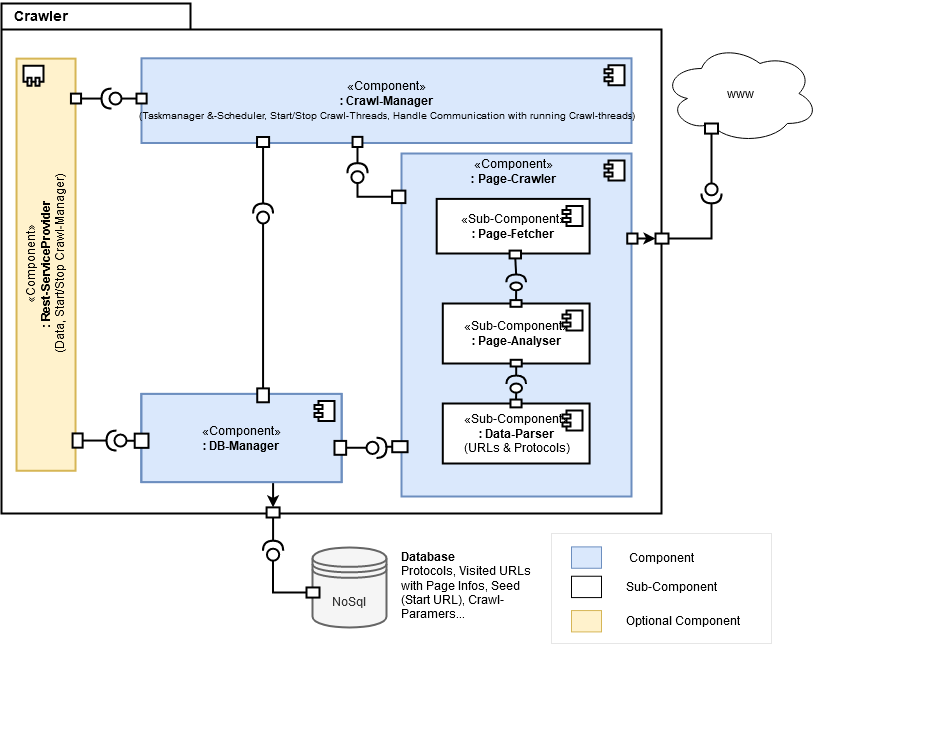
\includegraphics[width=5in]{images/02-Crawler/Crawler-Component-Diagram.png}
    \caption{Crawler: Komponentendiagramm}
    \label{fig:crawlerKompoenenten}
\end{figure}
\noindent
Am Ende eines Crawl-Prozess, bei dem neue Protokolle oder Stammdaten geladen worden sind, wird die Gruppe-Kommunikationsmodell die Liste aller Protokollen sowie Stammdaten über deren Rest-API~\cite{Cme2021} als Json-Datei mitgeteilt. Die Gruppe-Kommunikationsmodell kann dann asynchron die entsprechenden Dateien aus unseren Datenbank holen.
\section{Implementierung und Bereitstellung der Lösung}\label{sec:02_04_implementierung_bereitstellung}

\subsection{Implementierung des Crawlers}
Für die Umsetzung des Crawler wurde die Entscheidung getroffen eine Web-Anwendung (Rest-Schnittstelle, Crawl-Prozess und Scheduler) zu bauen. Dafür wurde Spring Boot~\cite{SpringBoot242} als Java-basierender Framework für die Entwicklung von Web-Anwendungen gewählt. Damit lassen sich Konfigurationen (für Rest-APIs, Datenbanktreiber, etc.) mit Hilfe des Spring-Initializers vereinfachen. Außerdem verfügt Spring Boot über einen eigenen Task-Scheduler der für den Crawl-Manager verwendet werden kann. Die finale Lösung beinhaltet vier Packages: \textbf{crawler} mit den Funktionalitäten für den Crawl-Prozess und das Parsen, \textbf{models} und \textbf{repositories} für den DB-Manager und \textbf{web} mit den Controllers für die Rest-Schnittstelle und den Services für den Crawl-Manager. Das gesamte Projekt-Verzeichnis inkl. Code ist auf dem Github-Repository \textit{Sentiments-of-Bundestag/Crawler}~\cite{Crawler2021} zu finden. Dort kommt unter anderem für die Ausführung Javascript-basierende Inhalte für den Download bestimmter Teile (Protokoll-Slides) der Webseite die \\\textbf{HtmlUnit}-Bibliothek~\cite{HtmlUnit2021} zum Einsatz (siehe ~\ref{subsubsec:techAnforderungen}).

\subsection{Bereitstellung der Lösung}
Der Crawler wurde auf dem Virtual-Server der Gruppe 1 (141.45.146.161) an der HTW (nur im HTW-Netz sichtbar) als Ubuntu-Service bereitgestellt. Der Crawler-Service liefert eine Rest-Schnittstelle, die jedoch nur auf dem infosys1 Rechner aus Sicherheitsgründen zugänglich ist. Die Konfiguration des Crawler-Services, die unter \textit{/etc/systemd/system/crawler.service} angelegt wird, sieht wie folgt aus (Start des Crawlers: systemctl enable crawler):
\begin{lstlisting}
[Unit]
Description=Crawler App
...
User=local
[Service]
ExecStart=/usr/bin/java -jar ../Crawler-1.0-SNAPSHOT.jar
Restart=always
SyslogIdentifier=crawler
...
[Install]
WantedBy=multi-user.target
\end{lstlisting}
Da für den Crawler eine MongoDB benötigt wird, soll diese auch bei der Bereitstellung konfiguriert werden. Dabei muss sichergestellt werden, dass der zugriff auf die Datenbank nur mit den entsprechenden Zugangsdaten erfolgt. Also soll nach dem Hinzufügen eines neuen Admin-User die Security-Konfiguration von mongod unter \textit{sudo nano /etc/mongod.conf} auf \textit{authorization: enabled} umgestellt werden. Da die MongoDB von der Gruppe 2 (Kommunikationsmodell) verwendet wird, sollen dafür entsprechend die Firewall-Regeln angepasst werden. Der nachfolgende Auszug aus unserer Konfiguration-Datei (/root/Firewall.sh) zeigt wie dies beispielhaft erfolgen sollte.
\begin{lstlisting}
...
#
# Erlaube zugang im 145.45.x.x port 27017 MongoDB
#
iptables -A INPUT -s 141.45.0.0/16 -p tcp -m tcp --dport 27017 -j ACCEPT
...
\end{lstlisting}

Der bereitgestellten Crawler basiert auf Java 11 und ist somit eine Plattform-unabhängige Lösung, die auf allen Betriebssystemen angeboten werden kann. Die Steuerung des Crawlers erfolgt ausschließlich über die Rest-Schnittstelle mit folgenden Abfragen (hier mit curl in der Shell-Konsole):
\begin{lstlisting}
# opendata: https://www.bundestag.de/services/opendata
# Start a default crawl to opendata
$ curl -X POST http://localhost:8080/task/default
# Start the default cron process to opendata: Mon - Fri, 23
$ curl -X POST http://localhost:8080/task/cron
# List all running tasks
$ curl -X GET http://localhost:8080/tasks 
# Cancel planed task
$ curl -X POST http://localhost:8080/task/cancel/{task_id}
# Cancel all planed tasks
$ curl -X POST http://localhost:8080/tasks/cancel
\end{lstlisting}

Der Crawler auf dem infosys1-Server (infosys1.f4.htw-berlin.de) läuft seit dem 27.11.2020 mit ein Paar Unterbrechungen für Aktualisierungen problemlos und konnte zum Zeitpunkt der Verfassung dieser Dokumentation schon 204 Protokollen herunterladen, parsen und in der MongoDB speichern, Stammdaten von 4.086 Abgeordneten sammeln und dabei mehr als 500 Urls durchsuchen. Was den Datenaustausch mit anderen Gruppen angeht, konnte bis jetzt erfolgreich durch Gruppe 2 auf unsere MongoDB zugegriffen werden und Mitteilungen von neu gecrawlten Daten konnten fehlerfrei zugestellt werden.\\
Aus den vom Crawler gesammelten Daten wird nun durch Gruppe 2 ein Kommunikationsmodell gebaut, das von den anderen Gruppen für weitere Verarbeitungen und Analysen verwendet wird. Der Aufbau dieses Kommunikationsmodells wird nun von Gruppe 2 im nächsten Kapitel aufgegriffen. 

\chapter{Kommunikationsmodell}
\section{Einleitung}
\label{sec:03_01_einleitung}

Im Rahmen des Projekts \gls{sob} sollten Bundestagsprotokolle analysiert
werden, um den \enquote{Ton} des Bundestags zu bewerten. Das in diesem
Kapitel beschriebene Teilprojekt, das von Gruppe 2 bearbeitet wurde, hatte
die Wahl und Anwendung eines passenden Kommunikationsmodells zum Ziel. Zur
Erfüllung dieser Zielstellung wurde die \enquote{\gls{cme}}-Software erstellt.
Diese ist das letzte Pipeline-Element des Gesamtprojektes, das sich mit den Rohdaten der
Bundesregierung beschäftigt. Die in diesem Teilprojekt generierten Daten
stellen die Basis aller weiteren Verarbeitungsschritte dar.

\subsection{Zielstellung}
Die \gls{cme}-Software soll aus den \citetitle{OpenData2019}~\cite{OpenData2019}
\todo{check that we are not the first ones using it otherwise use enquotes}
\gls{xml}-Dateien der 19. Wahlperiode des Bundestages bzw. der leicht
abgewandelten Variante dieser Daten, welche von Gruppe 1 in Form von
\gls{json}-Dateien zur Verfügung gestellt werden, Interaktionen zwischen
Fraktionen und oder Abgeordneten extrahieren.

Für diese Extraktion werden die Rohdaten analysiert und darauf aufbauend ein
passendes Kommunikationsmodell gewählt. Um über neue Protokolle von Gruppe 1
informiert werden zu können, soll dafür eine Schnittstelle geschaffen werden.
Ebenfalls werden zur Weitergabe der Ergebnisse an die folgende Gruppe ein
Datenmodell, welches zur Speicherung der Ergebnisse dient, eine Schnittstelle
zur Weitergabe der Daten und eine weitere Schnittstelle, über welche Gruppe 3
bei neuen Daten benachrichtigt werden kann, entwickelt.

\subsection{Anforderungsdefinition}

Auf Grundlage der im vorherigen Abschnitt beschriebenen Zielsetzung sowie der
Diskussionen in den Plenarsitzungen während des Semesters, erfolgt in diesem
Kapitel eine Zusammenfassung von funktionale Anforderungen, welche an das zu
entwickelnde System gestellt werden. Diese werden in Muss-, Soll- und
Kann-Kriterien unterteilt.


\begin{table}[H]
    \caption{Funktionale Anforderungen}
    \vspace{0.5cm}
    \renewcommand{\arraystretch}{2.5} % Default value: 1
    \centering
    \begin{tabularx}{\textwidth}{c|c|X}
                                & \textbf{FR01} & \noindent\parbox[c]{\hsize}{
                                                  Ein passendes Kommunikationsmodell und
                                                  Datenmodell muss gewählt werden} \\
                                & \textbf{FR02} & \noindent\parbox[c]{\hsize}{
                                                  Das Ausgabeformat von Gruppe 1 muss eingelesen
                                                  werden können} \\
                                & \textbf{FR03} & \noindent\parbox[c]{\hsize}{
                                                  Interaktionen basierend auf den Kommentaren
                                                  zu Redebeiträgen müssen extrahiert werden} \\
                                & \textbf{FR04} & \noindent\parbox[c]{\hsize}{
                                                  Extrahierte Interaktionen müssen für den
                                                  Zugriff späterer Gruppen persistiert werden} \\
        \textbf{Muss-Kriterien} & \textbf{FR05} & \noindent\parbox[c]{\hsize}{
                                                  Spätere Gruppen müssen auf die persistierten
                                                  Nachrichten zugreifen können} \\
                                & \textbf{FR06} & \noindent\parbox[c]{\hsize}{
                                                  Gruppe 1 muss die Möglichkeit haben, uns über
                                                  die Verfügbarkeit neuer Daten zu
                                                  benachrichtigen} \\
                                & \textbf{FR07} & \noindent\parbox[c]{\hsize}{
                                                  Gruppe 3 muss von uns benachrichtigt werden,
                                                  wenn neue Daten zur Verfügung stehen} \\
                                & \textbf{FR08} & \noindent\parbox[c]{\hsize}{
                                                  Parteien und Abgeordnete müssen über Sitzungen
                                                  hinweg eindeutig zuordenbar sein} \\
                                & \textbf{FR09} & \noindent\parbox[c]{\hsize}{
                                                  Daten von Gruppe 1 müssen aus deren MongoDB
                                                  ausgelesen werden können} \\
        \hline

        \textbf{Soll-Kriterien} & \textbf{FR10} & \noindent\parbox[c]{\hsize}{
                                                  Das Open Data Ausgabeformat des Bundestags soll
                                                  eingelesen werden können} \\
        \hline

        \textbf{Kann-Kriterien} & \textbf{FR11} & \noindent\parbox[c]{\hsize}{
                                                  Interaktionen innerhalb der Redebeiträge können
                                                  extrahiert werden} \\

    \end{tabularx}
    \label{tab:03_requirements}
\end{table}


\subsection{Wahl des Kommunikationsmodells}
FR01 erfordert die Auswahl eines passenden Kommunikations- und Datenmodells.
Aus diesem Grund wurden zu Beginn des Semesters die bereits vorliegenden
Plenarprotokolle im \enquote{\citetitle{OpenData2019}}-Format der
Bundesregierung untersucht.

Bei dieser Untersuchung zeigte sich, dass die für uns interessanten Daten so
angeordnet sind, dass jede Sitzung in Tagesordnungspunkte unterteilt ist,
welche wiederum aus einer Vielzahl von Reden besteht. Eine solche Rede
enthält dabei Informationen über den Redner, die in einzelne Absätze
zerteilte Rede und optionale Kommentare anderer Parlamentarier oder
Fraktionen zu diesen Absätzen. So sind in diesen Strukturen Interaktionen
erkennbar, z.~B. in den Kommentaren an den Redner gerichtete Interaktionen oder
auch in den Absätzen Interaktionen zwischen dem Redner und anderen
Parlamentariern.

Basierend auf diesen Erkenntnissen und in Absprache mit Gruppe 3, 4 und 5,
welche für die Sentimentanalyse sowie die Auswertungen zwischen Fraktionen und
Abgeordneten verantwortlich sind, wurde ein Sender-Empfänger-Modell für die
Repräsentation der Interaktionen gewählt. In diesem kann der Sender und
Empfänger jeweils entweder ein Bundestagsabgeordneter oder eine Fraktion sein.
Auf Basis des Inhalts der Nachricht, die vom Sender zum Empfänger geschickt
wird, wird später von Gruppe 3 das Sentiment ermittelt.

\section{Umsetzung}\label{sec:03_02_umsetzung}
Auf Grundlage der definierten Anforderungen wurde im nächsten Schritt ein
Konzept für deren Umsetzung entwickelt. Dieses sowie die Umsetzung selbst
wird in den folgenden Abschnitten näher erläutert.

\subsection{\glsentryfull{cme}}
Für die Entwicklung der \gls{cme}-Software wurde die Programmiersprache Python
gewählt, da alle Teammitglieder bereits Kenntnisse in dieser mitbrachten und
um den folgenden Gruppen möglichst schnell erste Ergebnisse liefern zu können,
mit denen diese arbeiten können. So bietet Python eine Vielzahl an guten und
einfach zu nutzenden Bibliotheken, welche die Entwicklung einer solchen
prototypischen Applikation beschleunigen können. Z.~B. ist es innerhalb
weniger Zeilen möglich, einen funktionsfähigen \gls{rest}-Endpoint zur
Verfügung zu stellen.

Aus den funktionalen Anforderungen FR05, FR06 und FR07 ergibt sich, dass eine
Kommunikation zu den Gruppen 1 und 3 nötig ist. Aufgrund hoher Kompatibilität
wurde sich für eine \gls{rest}-Schnittstelle entschieden. Diese \gls{api} wurde in dem
Python-Modul \enquote{api.py} mithilfe der FastAPI-Bibliothek implementiert. Sie
beantwortet Anfragen zu Protokollen (Sessions) Fraktionen (Factions) und
\glspl{mdb}. Außerdem wird eine SWAGGER-Dokumentation
bereitgestellt.

Zur Steuerung der Anwendung wird ein \gls{cli}, welches im \enquote{cli.py}-Modul umgesetzt
wurde, in Form der \gls{cme}-Applikation zur Verfügung gestellt. Dieses ist in
verschiedene Unterkommandos aufgeteilt. Mithilfe dieser ist es z.B. möglich
Protokolle manuell aus dem lokalen Speicher einzulesen (\gls{xml}- oder \gls{json}-Format)
oder den Server zu starten. Mit \enquote{init} werden erstmalig Bundestagsabgeordnete
eingelesen. \enquote{dump} ermöglicht die Interaktion mit der Datenbank, um einzelne
Dokumente daraus zu extrahieren.

Um die Anwendungslogik von der Business-Logik zu trennen, wird der \enquote{Controller}
eingeführt. Es ist das zentrale Modul, welches die Prozesse koordiniert.

Für die generische Verarbeitung der Rohdaten in den verschiedenen Datenformaten
von Gruppe 1 (FR02) und der Open Data Protokolle des Bundestags (FR10) wurde
das \enquote{Data}-Modul implementiert. Dieses wandelt die Rohdaten unter anderem in
sogenannte InteractionCandidates um, welche dann mithilfe des \enquote{Extraction}-
Moduls verarbeitet und ausgewertet werden (FR03 und FR11). So extrahiert dieses
aus den InteractionCandidates die stattgefundenen Interaktionen basierend auf
dem Sender-Empfänger-Modell und legt diese in einem sogenannten Transcript ab.
Dieses Transcript wird anschließend mithilfe des \enquote{Database}-Moduls, welches für
jeglichen Datenbankzugriff zuständig ist, in der Datenbank abgelegt.

Zuletzt enthält \enquote{Domain} Datenmodelle für verschiedene Objekte, wie z.~B. \gls{mdb},
Faction \& Interaction. Es wird von so gut wie jedem Modul benutzt.

Die soeben beschriebenen Module und der damit verbundene Kontrollfluss zwischen
diesen ist in \autoref{fig:03_project_structure} dargestellt.

\begin{figure}[ht]
    \begin{center}
        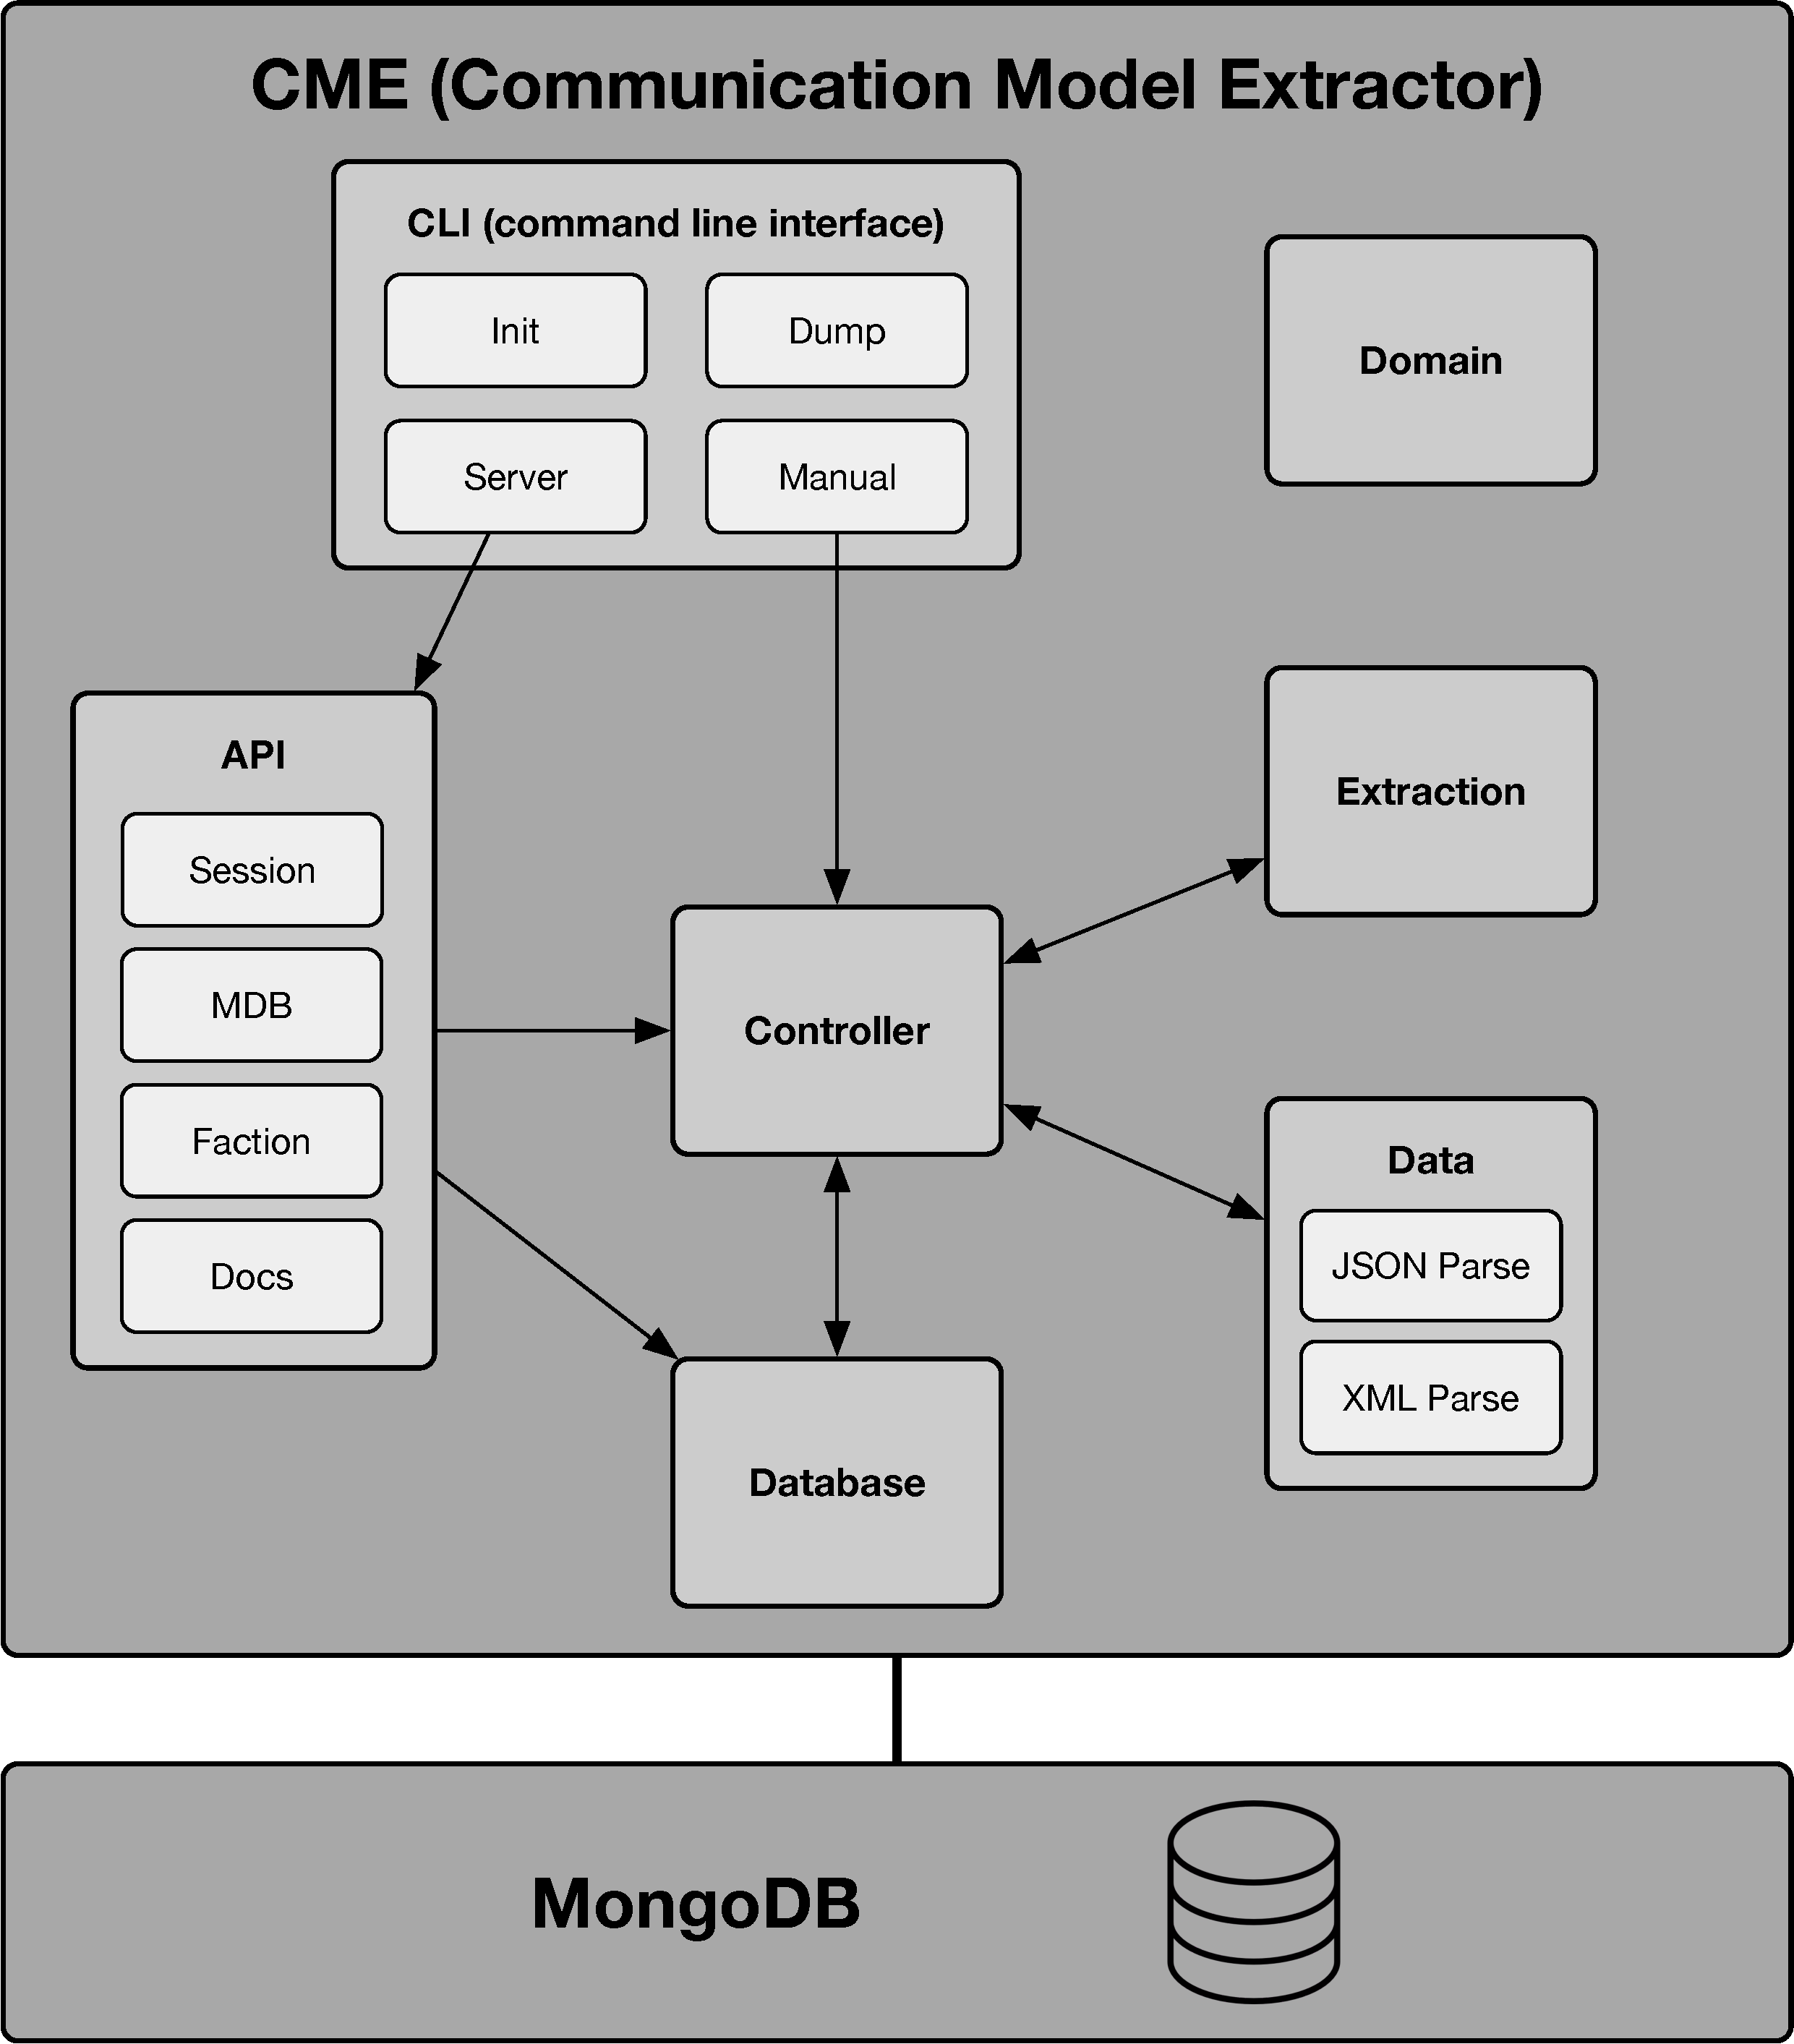
\includegraphics[width=0.6\textwidth]{images/03-cme/Project-Modules.pdf}
    \end{center}
    \caption{Applikations-Architektur}
    \label{fig:03_project_structure}
\end{figure}

\subsection{Eingabeformate}
Wie in den Anforderungen FR02 und FR10 definiert, muss als Eingabeformat
einerseits das \gls{json}-Format der Gruppe 1 und andererseits soll auch das
Open Data \gls{xml}-Format des Bundestags unterstützt werden. So wurden
spezielle Parser für die jeweiligen Formate entwickelt, deren Ausgabe gleich
formatiert ist und somit für die nächste Instanz eine einheitliche
Schnittstelle bildet. Dieses Ausgabeformat enthält dabei neben Metadaten zur
Sitzung selbst, wie z.~B. den Sitzungsstartzeitpunkt oder die Sitzungsnummer,
sogenannte InteractionCandidates. Diese gruppieren, wie der Name bereits
nahelegt, Daten, welche eventuelle für die Auswertung relevante Interaktion
enthalten. So gruppiert ein InteractionCandidate den Redner (Speaker),
einen Absatz von dessen Rede (Paragraph) und den eventuell darauf folgenden
Kommentarblock (Comment).

\subsection{Methodik der Kommunikations-Analyse}
Die zu analysierenden Daten (InteractionCandidates) bieten zwei verschiedene
Kommunikationstypen als Datengrundlage für die Erkennung von Interaktion:

\begin{enumerate}
    \item \textbf{Kommentare (FR03)}: werden von den Redeteilen gesondert
        dargestellt und mit zusätzlicher Information bezüglich der
        kommunikativen Einordnung des Beitrags versehen.
    \item \textbf{Redeteile (FR10)}: werden in den Protokollen als
        Paragraphen oder sinngemäß als Absätze aufgeführt.
\end{enumerate}

Aufgrund der Unterschiedlichkeit mussten beide Typen gesondert analysiert werden.

\subsubsection{Kommentare}

Kommentare werden nach rigiden strukturellen Regeln in den Protokollen der
Bundestagssitzungen erfasst und liefern unter anderem Informationen zum
Sender des Kommentars. Dieser kann eine oder mehrere Fraktionen oder eine
oder mehrere an der Sitzung teilnehmende Personen sein. Kommentare lassen sich
in die Folgenden drei Kategorien unterteilen:

\begin{itemize}
    \item \textbf{Publikumsresonanzen}: Z.~B. Beifall oder Entrüstung des
        Senders, bei der eine genaue Zitierung durch die Stenographen nicht
        möglich ist. Hier folgen Sender durch Präpositionen abgetrennt auf
        den Kommentarinhalt. Bsp.: \enquote{Beifall bei der CDU};
        \enquote{Zurufe von der Linken und Grünen}

    \item \textbf{Zitate}: Hier wird der Wortlaut eines Kommentars
        wiedergegeben. Bei diesen Kommentaren wird die kommentierende Person
        dem Wortlaut vorangestellt und durch einen Doppelpunkt abgetrennt.
        Bsp.: \enquote{Dr. Klaus Hermann: Ganz toll gemacht}; \enquote{Dr.
        Alexander Gauland: Schwachsinn}

    \item \textbf{Beobachtungen der Protokollanten}: Spezielle Situationen in
        denen ein oder mehrere Sitzungsteilnehmer nennenswerte Handlungen
        vornehmen. Auch hier wird in der Regel der Sender der Nachricht
        vorangestellt, wenngleich keine Trennung durch einen Doppelpunkt
        erfolgt. Bsp.: \enquote{Manfred von Kuchenhausen verlässt die Sitzung}

\end{itemize}

Je nach erkannter Kommentarform kommen also verschiedene strukturelle
Analyse-Vorgänge für die Feststellung von Sendern zum Einsatz.

\paragraph{Kommentare mit abweichender Struktur}

Es gibt weitere Eigenschaften, die die Extraktion der Interaktionen
erschweren. So können pro Kommentar-Abschnitt mehrere Strukturen mit
unterschiedlichen Inhalten auftreten, oder es werden insbesondere bei
Publikumsresonanzen mehrere Absender aufgeführt (etwa
\enquote{Beifall von SPD und die Linke}), wodurch zusätzlich eine korrekte
Auftrennung der Sender auf Basis von Konjunktionen bzw. Interpunktion
notwendig wird. Außerdem gibt es gelegentlich sekundäre Kommentare, bei denen
auf vorherige Kommentare reagiert wird. Die einzigen zuverlässigen
Formatierungen, die auf solche Verhältnisse hinweisen, sind die expliziten
grammatikalischen Strukturen nach der Namensnennung:
\enquote{an [neuer Empfänger] gerichtet} bzw. \enquote{zur [Ziel-Fraktion] gewandt}
wirken innerhalb von Kommentaren als klares Merkmal für einen vom Redner
abweichenden Empfänger. Das Schlüsselwort \enquote{Gegenruf} wird darüber
hinaus häufig verwendet, um auf einen Dialog zwischen Kommentierenden
hinzuweisen - da in diesen Fällen allerdings der Kommentarinhalt oft
mindestens teilweise weiterhin auf den Redner abzielt, wurde bei solchen
Kommentaren ebenfalls der Redner als Empfänger verwendet. Diese
Problematik könnte in Fortsetzungen der Arbeit eventuell präziser behandelt
werden, da in längeren Kommentar-Dialogstrukturen recht häufig auf die
eindeutige Empfängerbezeichnung verzichtet wird. Dadurch werden in unserer
Methode viele für menschliche Leser offensichtliche Interaktionen nicht als
solche registriert. Nicht zuletzt werden die genannten syntaktischen
Strukturen gelegentlich durch Rechtschreib- oder Zeichensetzungsfehler
durchbrochen, wobei in diesen Fällen die gesamte Interaktion verloren geht.

\subsubsection{Redeteile}
Redeteile besitzen weniger Struktur als Kommentare, da sie nicht den Regeln der
Stenographen unterliegen, sondern des individuellen Redners. So muss der
Empfänger einer Aussage erst ermittelt werden. Redeteile wurden daher auch nur
als Interaktionen gewertet, sobald Fraktionen oder Mitglieder des Bundestags
als mögliche Interaktionsempfänger im Fließtext erkannt wurden.

Die Erkennung von \glspl{mdb} erfolgt über die Feststellung bekannter, eindeutiger
Nachnamen, denen eine formale Anrede (Herr/Hr., Frau/Fr., Kollege, Doktor)
vorangeht. Parteien wurden anhand von ihren Namen bzw. deren Abkürzungen,
beziehungsweise durch gängige aber eindeutige Kurzformen identifiziert. Die
festgestellte Person oder Partei wurde anschließend als Empfänger der Nachricht
behandelt, während die sprechende Person, also der durch den
Sitzungspräsidenten zuletzt eingeleitete Redner, die Rolle des Absenders
einnahm.

Die Empfängerermittlung bei Redeanteilen verblieb in der entstandenen
Implementierung in einem recht rudimentären Zustand, da viele der inhärenten
Probleme des Ansatzes nicht behandelt werden konnten. So konnte etwa die
Unterscheidung zwischen mehreren \glspl{mdb} mit gleichen Nachnamen oder die
kolloquiale Verwendung von Farben (\enquote{Rot} für SPD oder die Linke) oder
Begriffen (\enquote{Liberale} stellvertretend für die FDP) als Substitut für Fraktionen
nicht behandelt werden. Um diese Problematiken zu umgehen wurden in der
Paragraphen-Analyse nur solche Interaktionen gewertet, welche sich an eindeutig
identifizierbare \glspl{mdb} oder Fraktionen richten. Nachnamen wie \enquote{Müller}, die
mehrere \glspl{mdb} bezeichnen können, aber auch in anderen Sachverhalten eingesetzte
Begriffe, wie \enquote{Union}, wurden somit aus der Schlüsselwort-Liste entfernt, mit
der die Redeabschnitte abgetastet wurden. \todo{Dieses sehr spezielle Beispiel
vielleicht näher erläutern?} Auch die Nennung von Nachnamen als Referenz, etwa
bei Beiträgen, die an \glspl{mdb} gerichtete Morddrohungen thematisieren,
wurde im späteren Verlauf der Arbeit als Grund für Mängel in den Ergebnissen
identifiziert, in diesem Fall in der Form von fehlerhaften Interaktionen.
Durch diese Probleme wurde eine unbestimmt große Menge von Fehlern durch die
Redeteil-Analyse produziert, sowohl in nicht erkannten Interaktionen als auch in
fälschlicherweise als Interaktionen kategorisierten Beiträgen, was mit Sicherheit
eine Verzerrung der Projektergebnisse, aber gleichzeitig auch ein wesentliches
Verbesserungspotential für mögliche Fortsetzungen dieses Teilprojekts
darstellt. Gleichzeitig sollte nicht außer Acht gelassen werden, dass
Interaktionen in Redeteilen nach unseren Messungen einen recht geringen Anteil
der Interaktionen im Bundestag ausmachen. Die Steigerung der Anzahl erkannter
Interaktionen durch unsere Methode der Redebeitrag-Analyse betrug für die
bisherigen Protokolle der 19. Wahlperiode lediglich 8\% gegenüber der alleinigen
Betrachtung der Kommentare.

\subsection{Ermittlung von teilnehmenden Personen}
Personen müssen über Sitzungen hinweg eindeutig identifizierbar sein, damit
nachfolgende Gruppen Informationen zu Parteizugehörigkeit und Namen korrekt
zuweisen können (FR08). Personen werden in der \enquote{mdb}-Collection der MongoDB
gesammelt. Initialisiert werden kann diese Liste mithilfe der Stammdaten der
Bundestagsabgeordneten des Bundestags. Diese als \gls{xml} zur Verfügung gestellte
Liste enthält alle relevanten Informationen, die bei der Identifizierung
helfen (Namen und Namensänderungen, Parteizugehörigkeit mit von-bis-Datumsangabe,
Titel etc.).

Da die Stammdaten unvollständig sind, auch weil Gastredner Reden halten oder
Bundestagsabgeordnete in den Stammdaten fehlen, müssen weitere Redner während
der Analyse hinzugefügt werden. Gerade in den Kommentaren können meist Vor-
und Nachnamen extrahiert werden, um ein Abgleich mit den \gls{mdb}-Daten
vorzunehmen. Leider werden Namen oft inkonsistent geschrieben (z.~B. wird
der zweite Vorname manchmal ausgeschrieben, abgekürzt oder weggelassen) oder
die Stenographen vertippen sich. Auch wird das Format der Kommentarsektion
nicht immer eingehalten.

Weil fehlende Redner und Rechtschreibfehler nicht unterschieden werden können,
gelangen doppelte Einträge in die Datenbank. Es wurden Mechanismen eingebaut,
um solche Fehler zu erkennen. Diese können jedoch nicht ganz ausgeschlossen werden.

\subsection{Infrastruktur-Setup mit Docker}
Um ein einfaches Deployment zu ermöglichen, wurde ein Container-basierter
Deploymentansatz gewählt. Dieser nutzt sowohl einen Container für die im
Rahmen des Teilprojektes erstellte Software als auch für die MongoDB, welche
für die Persistierung der Daten genutzt wird.

Die beiden Container werden mithilfe von docker-compose verwaltet und
konfiguriert. Dabei gibt es neben der docker-compose-Konfiguration für das
Deployment auch eine zweite für die lokale Entwicklung. Diese enthält primär
die MongoDB, da während der Entwicklung der lokale Code mit den entsprechenden
Modifikationen genutzt werden soll und z.~B. ein ständiges Neubauen des
Applikation-Images und damit unnötiger Zeitaufwand verhindert werden soll.

Die Konfiguration des MongoDB-Containers erfolgt über Environment-Variablen
und ein \textit{mongo-init.sh}-Skript, welches beim ersten Starten des
Containers von dem MongoDB-Server ausgeführt wird. Dieses legt basierend auf
Environment-Variablen einen neuen DB-User (cme) an, welcher nur in einer
Datenbank mit dem Namen \textit{cme\_data} Lese- und Schreibrechte hat.

Das Applikation-Image wird bei jedem Starten der docker-compose-Umgebung
frisch gebaut und enthält die \gls{cme}-Software, welche durch die Tatsache,
dass es sich dabei um ein installierbares Python-Package handelt, einfach nur
dort installiert werden muss.

Zusätzlich wurde die Deployment-docker-compose-Konfiguration so konfiguriert,
dass ein Zugriff auf die Container von außen nicht möglich ist. Dies bedeutet
einerseits, dass der DB-Port des MongoDB-Containers nur durch den
\gls{cme}-Container erreichbar ist und andererseits, dass die
\gls{rest}-Endpoints des \gls{cme}-Containers nur über eine Verbindung von
Localhost aus erreichbar sind. Der Zugriff von außen erfolgt über einen
zusätzlich konfigurierten nginx-Reverse-Proxy. Dieser hat neben \gls{ssh} den
einzigen nach außen hin geöffneten Port auf dem Server. Somit muss jeder
Request durch diesen Reverse-Proxy fließen, bevor er in die
docker-compose-Umgebung gelangt.

\subsubsection{Datensicherheitsvorfall}

Während der initialen Konfiguration der Infrastruktur wurde der interne
Kommunikationsport des genutzten MongoDB-Containers aufgrund einer
fehlerhaften docker-compose-Konfiguration durch den Docker-Daemon nach außen
geöffnet und nicht, wie gedacht, nur lokal. So konnte auf die so für den Rest
des Internets frei zugängliche MongoDB von außen zugegriffen werden und diese
wurde kompromittiert.

Nachdem diese Situation dem Team bekannt wurde, wurde dies den entsprechenden
Parteien gemeldet und das System wurde ein zweites Mal aufgesetzt. Für diese
zweite Konfiguration wurde ausgiebig die vorliegende
docker-compose-Konfiguration überprüft. Dabei stellten wir fest, dass die
Verwendung des \textit{ports}-Arguments ohne die Angabe einer expliziten \gls{ip},
wie es in vielen docker-compose-Tutorials zu finden ist, dazu führt, dass der
Docker-Daemon diesen Port mithilfe einer zusätzlichen \gls{ip}-Tables-Chain nach
außen hin öffnet. Aus diesem Grund wurde in der offiziellen Dokumentation als
Lösung nach alternativen Möglichkeiten gesucht, Ports freizugeben. Dort wurde
einerseits die bereits erwähnte Lösung gefunden, welche durch die explizite
Angabe einer \enquote{Bind}-\gls{ip}-Adresse wie z.~B. hier
\enquote{127.0.0.1:9001:9001} dazu führt, dass nur Anfragen, die über diese
Adresse erfolgen, beantwortet werden. Andererseits wurde das
\textit{expose}-Argument entdeckt, welches diesen Port nur für alle
Docker-Container innerhalb derselben docker-compose-Umgebung freigibt.

Zur vollständigen Beseitigung des Problems wurde schließlich, wie auch schon
im vorherigen Abschnitt beschrieben, das \textit{expose}-Argument genutzt,
um den MongoDB-Container nur innerhalb der docker-compose-Umgebung zugänglich
zu machen. Zusätzlich wurde das Portbinding des \gls{cme}-Containers, welcher
den \gls{rest}-Service enthält, auf Localhost beschränkt. Die eigentliche
Auflösung von außen erfolgt dann über einen nginx-Reverse-Proxy, welcher im
Hostsystem unter einem nicht privilegierten Nutzer läuft. So ist jeglicher
Zugriff auf die docker-compose-Umgebung von außen nicht mehr möglich und muss
durch den Reverse-Proxy.

\subsection{Schnittstelle für Zugriff auf den Communication Model Extractor}

Um den gewünschten Workflow einer Pipeline zu ermöglichen, entschieden wir
uns eine \gls{api} anzubieten, wodurch die Kommunikation zur vorherigen und
folgenden Gruppe realisiert wurde.

\begin{figure}[ht]
    \begin{center}
        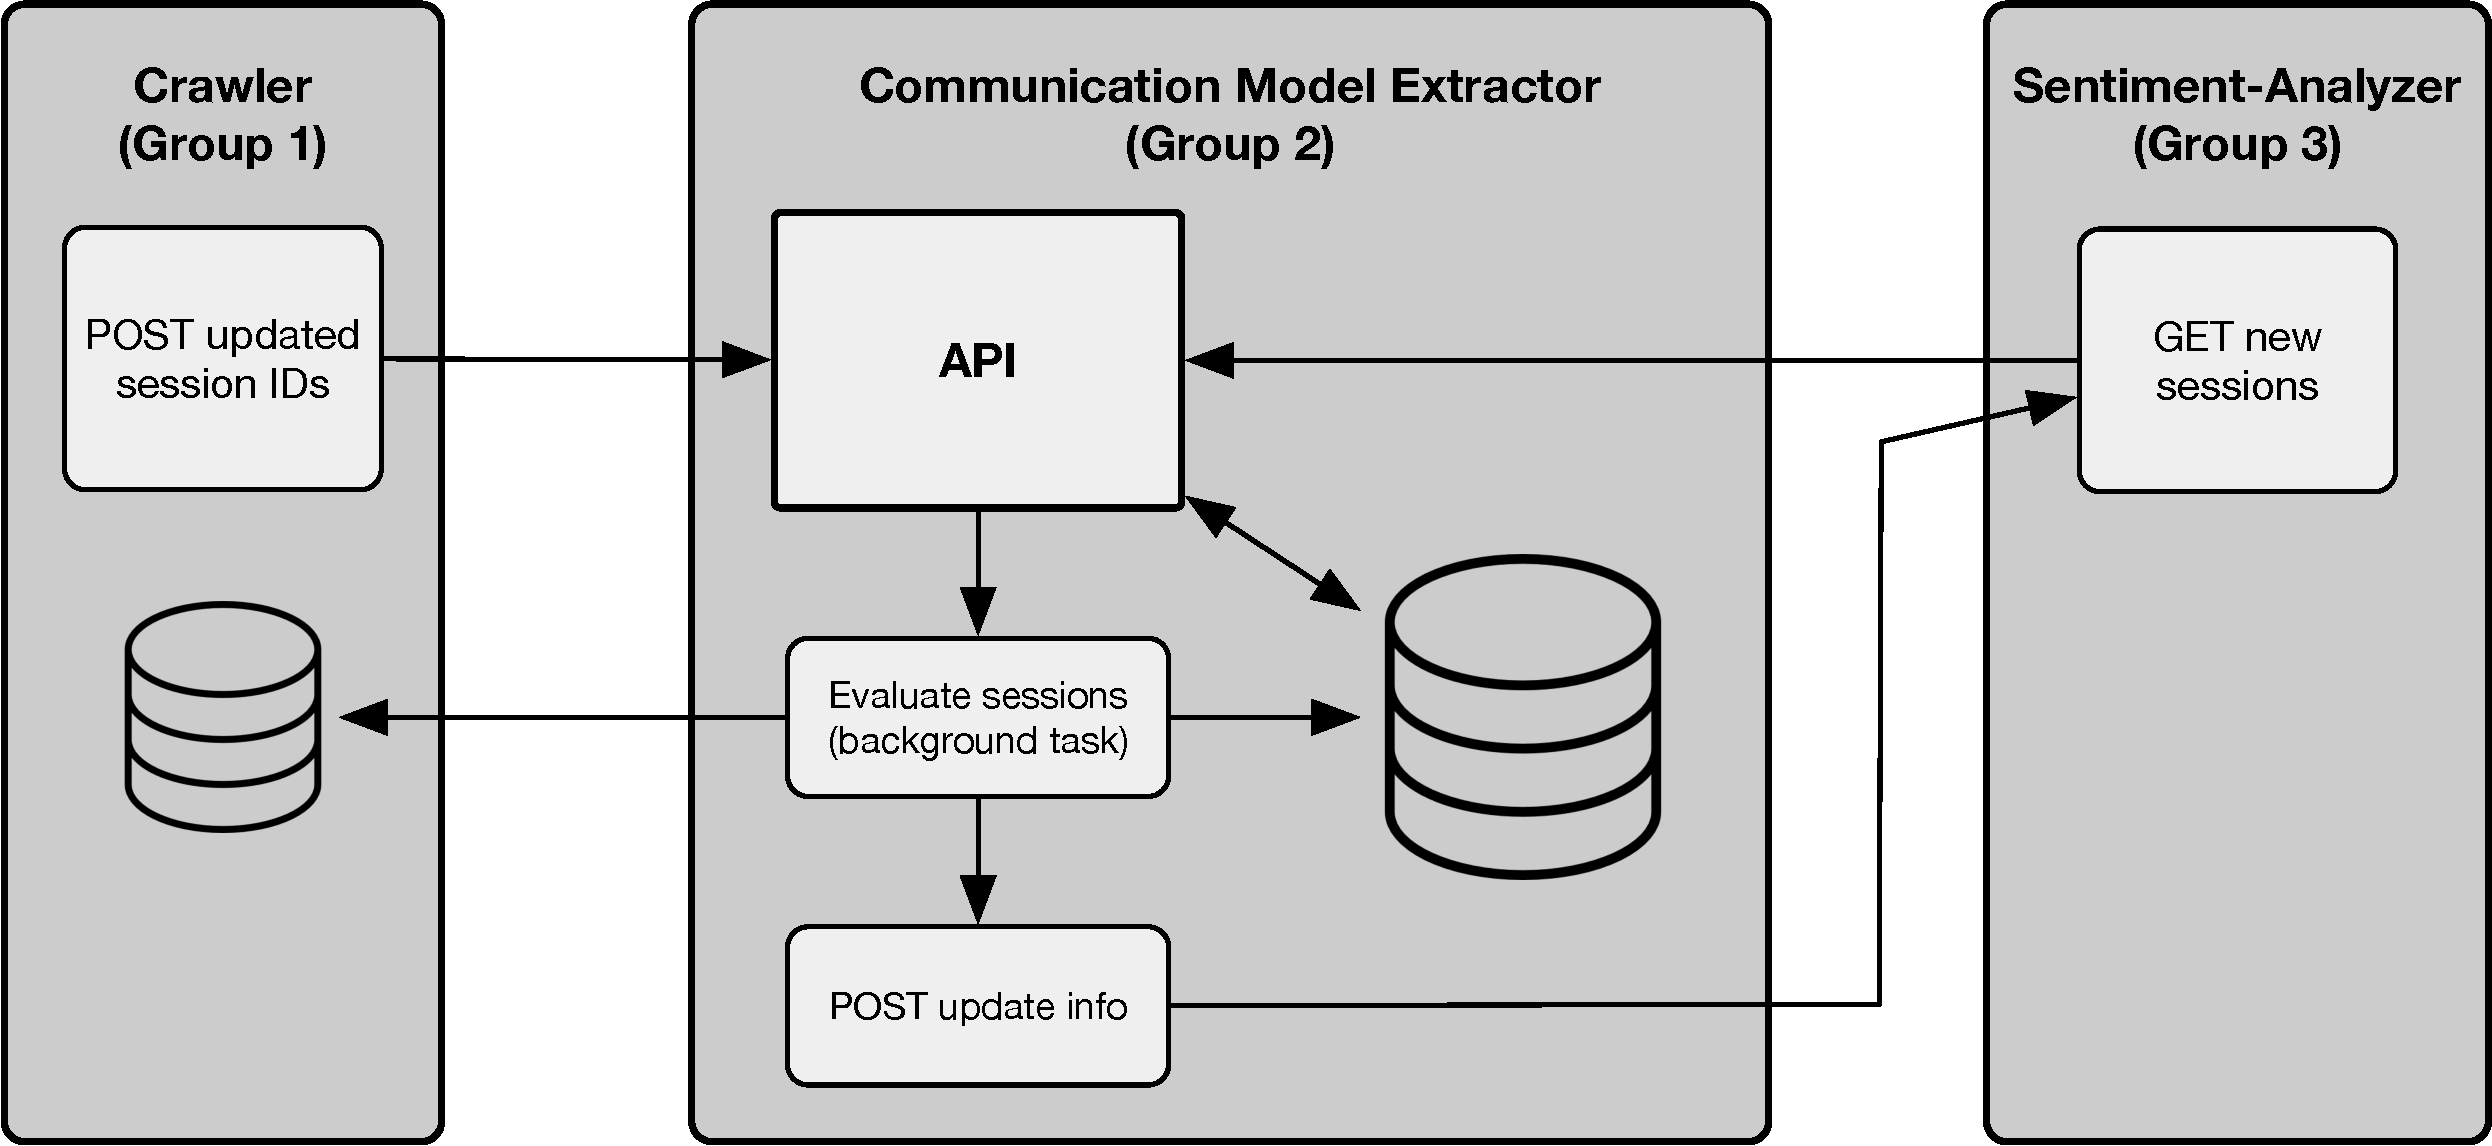
\includegraphics[width=\textwidth]{images/03-cme/Communications.pdf}
    \end{center}
    \caption{\gls{api}-Kommunikationsfluss}
    \label{fig:03_api_call_flow}
\end{figure}

Es wurde sich mit Gruppe 1 darauf geeinigt, dass der \gls{cme} einen Endpunkt
anbietet, um die Information zu erhalten, wenn neue Protokolle aus dem
Bundestag in deren Datenbank kreiert wurden. Zusätzlich bekamen wir
Zugangsdaten, um auf deren Datenbank zugreifen zu können. So werden uns die
Protokoll-ID's an \url{http://infosys2.f4.htw-berlin.de:9001/cme/data/} gesendet
und der \gls{cme} holt sich die gewünschten Protokolle zu einem späteren Zeitpunkt
aus deren Datenbank. Danach kann die Auswertung geschehen.

Um der darauffolgenden Gruppe Bescheid zu geben, wird nach dem Prozess der
Auswertung ebenfalls eine HTTP Anfrage gesendet, in der über die neuen
Protokoll-ID's informiert wird. Unsere \gls{api} bietet dafür verschiedene Endpunkte
an, um an alle notwendigen Informationen zu gelangen.

Diese Endpunkte sind alle in einem Endpunkt festgehalten, die die \gls{api}
dokumentiert und hier abgerufen werden kann:
\url{http://infosys2.f4.htw-berlin.de:9001/cme/doc/docs}

Demnach enthält der \gls{cme} folgende Endpunkte:
\begin{itemize}
    \item /cme/data/sessions/ - damit wird eine Liste aller existierenden
        Sitzungen zurückgegeben
    \item /cme/data/session/\{session\_id\} - um eine bestimmte Sitzung mit den
        ermittelten Interaktionen zu erlangen
    \item /cme/data/mdb - nützlich, um nach Mitgliedern des Bundestags zu
        suchen, mithilfe der Query-Parameter mdb\_id, speaker\_id, forename
        \& surname kann gefiltert werden
    \item /cme/data/faction - damit können alle existierenden Fraktionen mit
        jeweiliger ID abgerufen werden
\end{itemize}

Der Server ist nur über das \gls{htw}-Netzwerk erreichbar. Zusätzlich ist die \gls{api} mit
Basic Authentication geschützt. Dadurch kann nur auf die Daten zugegriffen
werden, wenn sich mit Username und Passwort authentifiziert wird.

Es wurden drei Clients, sprich User, angelegt, die auf die \gls{api} zugreifen
dürfen. Je einer für die anderen Gruppen crawler\_client \& sentiment\_client und
cme\_admin für unser Team, um Testen zu können und bei Bugs der Ursache auf den
Grund gehen zu können.

\section{Fazit}\label{sec:03_05_fazit}

Im Rahmen des Teilprojektes konnte erfolgreich die Extraktion des
Kommunikationsmodells basierend auf den
\enquote{\citetitle{OpenData2019}}-\gls{xml}-Dateien sowie dem
\gls{json}-Format von Gruppe 1 umgesetzt werden. Dabei wurden alle in
\todo{add ref} definierten Anforderungen erfolgreich erfüllt. So wurde ...
\todo{continue}

Abschließend konnten die meisten \todo{welche nicht?} Anforderungen
erfolgreich umgesetzt werden.

Der Service bietet Schnittstellen zur vorherigen und nachfolgenden Gruppe und
sowie automatisierte Verarbeitungsmechanismen (notify). Auch die frühzeitige
Bereitstellung einer akzeptierten Kommunikations-Modellierung auf Basis der
\gls{xml}-Rohdaten konnte realisiert werden. Der Großteil des Datenbestands wird
analysiert, sodass sowohl Kommentare als auch Redeteile auf Kommunikationen
überprüft werden.

Allerdings verwirft der Service, aufgrund von Inkonsistenzen in der Syntax und
Rechtschreibung sowie aufgrund von fehlenden kontextbasierten
Analyse-Mechanismen, potenzielle Interaktionen. Während in Kommentaren primär durch
Abweichungen von Protokoll-Syntax und Rechtschreibfehler Probleme entstanden,
so fehlte in den Redeteilen oft die nötige Information, um die Empfänger von
Interaktionen eindeutig zu bestimmen. Daher mussten Interaktionen verworfen
werden und teils wurden in Kommentaren inkorrekt genannte Personen als
Personenduplikate in den Datenbestand aufgenommen.

Daher wurde das Ziel der Gruppe \enquote{Kommunikationsmodell} in Funktionalität und
Integration zwar erreicht, allerdings wird deutliches Verbesserungspotential
für die Extraktion von noch mehr Interaktionen und die Eliminierung von
Artefakten gesehen. \todo{what? das ist viel zu negativ}

Die ausgelieferte Deployment-Strategie und die Modulbeschreibungen in dieser
Dokumentation sollten bei der Weiterentwicklung des Projekts hilfreich sein.

\chapter{Sentiment Analyse}
\section{Einleitung}
Der Begriff \textit{Sentiment} stammt vom lateinischen Wort \textit{sentimentum} ab und bedeutet Empfindung oder Stimmung. 
In der Sentimentanalyse geht es um die Bestimmung eben jener Stimmung einer Meinungsäußerung. 
Anwendung findet sie etwa bei Produktbewertungen oder Beiträgen in sozialen Netzwerken. 
Die Stimmung wird durch die sog. Polarität beschrieben und kann positiv, negativ oder neutral ausfallen. 
Im Text-Mining wird sie im Intervall $\interval{-1}{1} = \{x \in \mathbb{R} | -1 \leq x \leq 1\}$ angegeben, wobei -1 sehr negativ, 1 sehr positiv und 0 neutral bedeuten. 

Grundlegend ist die maschinelle Sentimentanalyse entweder Wortlisten- oder Modell-basiert. 
Der Wortlisten-Ansatz kann als eine Sammlung von Worten und ihrer Polaritäten verstanden werden, anhand welcher die Stimmung berechnet wird. 
Dieser Ansatz wird weiter im Kapitel \ref{wortliste} beschrieben, da er in dieser Arbeit verwendet wurde. 

Bei der Modell-basierten Sentimentanalyse wird ein annotierter Satz-Korpus für das Trainieren einer künstlichen Intelligenz vorausgesetzt. 
Etwa für Twitter-Beiträge stehen solche Korpusse oder auch bereits trainierte Modelle zur Verfügung. 
Jedoch ist bei der Verwendung zur Analyse der Sitzungsprotokolle des Bundestages nicht mit zufriedenstellenden Ergebnissen zu rechnen, da sich verwendete Worte und Text- bzw. Satzbau zwischen diesen Domänen deutlich unterscheiden. 
Eine weitere Erläuterung zur Sprache im Bundestag wird in Kapitel \ref{sprachebundestag} gegeben. 

Ebenfalls werden die Komponenten zur Teilnahme an der Verarbeitungspipeline des Gesamtprojektes im nachfolgenden Kapitel \ref{g3daten} beschrieben. 

\section{Datenaustausch}
\label{g3daten}
\subsection{Datenimport}
Für das Erhalten von Daten wurde eine Methode implementiert, welche durch Angabe einer Sitzungs-ID die entsprechende Sitzung vom REST-API von Gruppe 2 abfragen kann. 
Diese Methode gibt jede Sitzung weiter an die in Kapitel \ref{g3textv} beschriebene Textverarbeitung und das Ergebnis schließlich an den in Kapitel \ref{g3export} beschriebenen Export-Code. 

Die Methode wird für zwei Fälle verwendet: 
Beim Normalfall sendet die Gruppe 2 eine Benachrichtigung mit einer Liste aller neuen Sitzungs-IDs an das REST-API im Code dieser Arbeit. 
Das REST-API wurde mit der Bibliothek \mintinline{latex}{Flask} \cite{g3_flask} entwickelt und besteht aus einer POST-Schnittstelle, welche auf dem von der HTW bereitgestelltem Server unter \textit{/notify} erreichbar ist. 

Das API wurde unter Zuhilfenahme von \mintinline{latex}{Flask.Blueprints} \cite{g3_flaskbp} entwickelt und wird von einem \mintinline{latex}{Waitress}-Webserver \cite{g3_waitress} bereitgestellt. 
Für jede Anfrage wird geprüft, ob Content-Type und Payload dem erwarteten JSON-Daten entsprechen. 
Sollte dies nicht der Fall sein, wird eine entsprechende Rückmeldung an den Sender zurückgegeben. 
Für jede erhaltene Sitzungs-ID wird die eingangs beschriebene Methode aufgerufen. 

Der zweite Fall wurde vor allem im Rahmen der voranschreitenden Entwicklung bei den in der Projektpipeline voranstehenden Gruppen verwendet. 
Statt auf eine Benachrichtigung zum Anstoßen des Datenimports zu warten, werden stattdessen alle Sitzungs-IDs vom REST-API der Gruppe 2 abgefragt und jede Sitzung vollständig neu importiert. 
Dieses Vorgehen hat den Vorteil, dass eventuell durch Arbeit am Code verpasste Benachrichtigungen nachgeholt werden und gleichzeitig Änderungen an den Daten übernommen werden können. 

\subsection{Datenexport}
\label{g3export}
Statt Arbeit in ein umfangreiches REST-API für die nachfolgenden Gruppen zu stecken, wurde für diese Arbeit ein reiner MongoDB-Ansatz verwendet. 
Auf dem zur Verfügung stehenden HTW-Server wurde dafür eine MongoDB Instanz aufgesetzt, welche nur aus dem HTW-Netz erreichbar und zudem nur mit Authentifizierung zugreifbar ist. 
Jede Sitzung ist hier als eine eigene Collection persistiert. 
Sobald neue Sitzungen importiert und verarbeitet wurden, werden diese zunächst mit dem MongoDB-Treiber \mintinline{latex}{PyMongo} \cite{g3_mongodb} in die Datenbank geschrieben. 
Anschließend werden die nachfolgenden Gruppen mit einem POST and die jeweilige REST-Schnittstelle benachrichtigt, dass neue Daten vorliegen. 
Diese greifen dann mit den zuvor versendeten Zugangsdaten direkt auf die Datenbank zu. 

Mit diesem Vorgehen konnte die Komplexität beim Zugriff auf die Ergebnis-Daten gesenkt werden, da es für nahezu alle gängigen Programmiersprachen einen intuitiven MongoDB-Treiber gibt. 

\section{Wortliste}
\label{wortliste}
Wie bereits in der Einleitung beschrieben, handelt es sich bei Wortlisten in der Sentimentanalyse um eine Liste von Worten und ihrer jeweiligen Polarität. 
Bei der Analyse eines Textes wird wortweise ein Abgleich mit dieser Liste durchgeführt und die Wort-Polarität bei einer Übereinstimmung für die Berechnung des Sentiments verwendet. 
Unterschiedliche Berechnungsformeln sind dabei denkbar und werden in Kapitel \ref{polberechnung} weiter besprochen. 
Für diese Arbeit wurden Wortlisten verschiedener Institutionen kombiniert und anschließend mit Synonymen erweitert. 
Ebenfalls wurde eine eigene Bundestags-Wortliste erstellt. 

Die Interest Group on German Sentiment Analysis (IGGSA) stellt eine umfangreiche Liste an Publikationen und Ressourcen zu Sentimentanalysen in der deutschen Sprache zur Verfügung \cite{g3_iggsa}. 
Hier wurden alle Referenzen auf die in dieser Arbeit verwendeten Quell-Wortlisten gesammelt. 
Für die Zusammenführung dieser Wortlisten wurden zunächst zwei Herangehensweisen evaluiert: 
Zum einen war die Erstellung eines eigenständigen Codes denkbar, welcher einmalig die Daten aus allen Quellen einliest, zusammenfasst und eine Ergebnis-Datei ausgibt. 
Diese Datei wäre eine Ressource für den eigentlichen Analyse-Code. 
Zum anderen könnte die soeben beschriebene Funktionalität jedoch auch direkt im Analyse-Code integriert und bei jedem Programmstart ausgeführt werden. 
Die kombinierte Wortliste würde somit nicht auf die Festplatte geschrieben, sondern im Arbeitsspeicher verbleiben, solange der Analyse-Code läuft. 
Wenngleich der zuerst beschriebene Ansatz offensichtlich weniger Rechenzeitaufwändig ist, wurde für diese Arbeit der zweite Ansatz gewählt. 
Dies wird vor allem mit Rechtsunsicherheiten bei der Arbeit mit den verschiedenen Lizenzen der Quelldateien begründet. 
Gleichzeitig arbeitet der Analyse-Code damit jederzeit mit dem aktuellen Stand der Quell-Wortlisten. 
Das Aufbauen der Wortliste dauert wenige Minuten. 

Für diese Arbeit wurden die folgenden Quell-Wortlisten verwendet: 

\begin{itemize}
\item \textit{SentimentWortschatz} (SentiWS) aus \glqq SentiWS - a Publicly Available German-language Resource for Sentiment Analysis\grqq (Universität Leipzig) \cite{g3_sentiws}
\item \textit{Multi-Domain Sentiment Lexicon for German} (Hochschule Darmstadt) \cite{g3_opm}
\item \textit{German Polarity Lexicon} aus \glqq Evaluation and extension of a polarity lexicon for German\grqq (Universität Zürich) \cite{g3_polcla}
\item \textit{morphcomp} aus \glqq Evaluating the morphological compositionality of pola-rity\grqq (Leibniz-Institut für Deutsche Sprache, Universität des Saarlandes) \cite{g3_morphcomp}
\end{itemize}

Aus diesen Quellen ergibt sich eine Wortliste mit etwa 14.000 einzigartigen Worten. 
Die Worte werden dabei mit der in Kapitel \ref{g3textv} beschriebenen Textverarbeitungspipeline lemmatisiert, also auf die Grundform zurückgeführt. 
Bei Überschneidungen wird ein Mittelwert über alle Polaritäts-Werte eines Wortes gebildet. 

Mithilfe des \textit{Open German WordNet} (OdeNet) \cite{g3_odenet} werden zu jedem Wort Synonyme gesammelt und ebenfalls der Wortliste hinzugefügt. 
Der Zugriff auf OdeNet geschieht dabei mit der python Bibliothek \mintinline{latex}{WN} \cite{g3_wn}. 
Die Verwendung dieser Bibliothek ist trivial, weshalb an dieser Stelle keine weitere Erläuterung gegeben wird. 
Die Wortliste wird durch das Hinzufügen von Synonymen um weitere rund 2.000 Worte erweitert. 

Wie bereits in der Einleitung erwähnt, wurde zudem eine eigene Bundes-tags-Wortliste erstellt. 
Hierzu wurden die 15.000 am häufigsten in den Sitzungsprotokollen vorkommenden Worte erfasst und analysiert. 
Dabei wurden jedoch nur jene Worte betrachtet, welche nicht bereits in der kombinierten Wortliste vorkommen. 
Ausgewählt wurden nur eindeutig positive oder negative Worte wie \textit{angemessen}, \textit{Bullshit}, \textit{Fehlentscheidung}, \textit{Milchmädchenrechnung}, \textit{Realitätsverweigerung}, \textit{Totalausfall} oder \textit{Verunglimpfung}. 
Insgesamt umfasst die Bundestags-Wortliste 217 Worte. 

Im Code wird der Zugriff auf die Wortliste mit der zentralen Klasse \mintinline{latex}{Lexicon} realisiert. 
Bei der Instanziierung der Klasse werden, wie im Vorherigen beschrieben, alle Wortlisten gesammelt, zusammengeführt und erweitert. 
Anschließend stellt die Klasse ein \mintinline{latex}{Dictionary} bereit, in welchem die Schlüssel die Worte und die Werte die Wort-Polarität angeben. 

\section{Textverarbeitung}
\label{g3textv}
Für die Textverarbeitung nutzt der Code dieser Arbeit vollständig die Funktionalitäten und Strukturen von \mintinline{latex}{spaCy} \cite{g3_spacy}. 
Die \mintinline{latex}{spaCy} Bibliothek stellt eine Textverarbeitungspipeline bereit, welche mithilfe eines vortrainierten Modells funktioniert. 
Für die deutsche Sprache wurde ein solches Modell mit dem TIGER Korpus der Universität Stuttgart trainiert. 
Der Korpus umfasst ca. 50.000 Sätze aus Texten der Frankfurter Rundschau. 
Die \mintinline{latex}{spaCy}-Pipeline besteht aus den folgenden Komponenten: 

\begin{itemize}
\item Tokenisierung (Text- und Satzzerteilung)
\item POS-Tagging (Wortartenerkennung)
\item Dependency-Parsing (Wortabhängigkeitenerkennung)
\item Lemmatisierung (Wortgrundformermittlung)
\item Entity-Recognition (Eigennamenerkennung)
\end{itemize}

Das Ergebnis der Pipeline ist ein \mintinline{latex}{Doc}-Objekt, welches das Ergebnis des gesamten in die Pipeline gegebenen Textes umfasst. 
Einzelne Sätze innerhalb des \mintinline{latex}{Doc}-Objektes werden mit \mintinline{latex}{Span}-Objekten beschrieben und einzelne Worte mit \mintinline{latex}{Token}-Objekten. 
Die Objekttypen besitzen jeweils eigene Methoden und Erweiterungsmöglichkeiten in Form von sog. \textit{extension attributes}. 

Sehr einfach und gleichzeitig umfangreich kann die \mintinline{latex}{spaCy}-Pipeline an die eigenen Bedürfnisse angepasst werden. 
So wurde die Berechnung des Sentiments eines Textes direkt an die Komponenten der Standart-Pipeline angehängt. 
Logisch unterteilt sich diese in die Komponenten:

\begin{itemize}
\item Negations-Erkennung (siehe \ref{neg-erkennung})
\item Verstärkungs-Erkennung (siehe \ref{ver-erkennung})
\item Polaritätsberechnung (siehe \ref{polberechnung})
\end{itemize}

Basis für das nachfolgende Kapitel \ref{neg-erkennung} ist dabei das Ergebnis des Depen-dency-Parsers von \mintinline{latex}{spaCy}. 
Dieser bestimmt die Abhängigkeiten zwischen den einzelnen Elementen eines Satzes. 
Diese Funktion gehört dem Themenbereich der Dependenzgrammatik an, in welcher gerichtete Beziehungen zwischen den Worten eines Satzes beschreibt werden. 
Ein Wort kann einen Vorgänger (Regent) und mehrere Nachfolger (Dependenten) besitzen. 
Die Gesamtheit der Beziehungen eines Satzes wird auch Abhängigkeitsbaum genannt. 

Zur Verdeutlichung soll die Abbildung \ref{steffi} dienen, welche mithilfe von \mintinline{latex}{spaCy.displaCy} erstellt wurde. 
Zu sehen ist hier der Abhängigkeitsbaum des Satzes \textit{\glqq Das ist doch fachlich Quatsch hoch sechs!\grqq}. 
An den gerichteten Kanten befindet sich die Angabe des Satzgliedes, unterhalb der Worte die Angabe der Wortart. 

\begin{figure}[htb]
\centerline{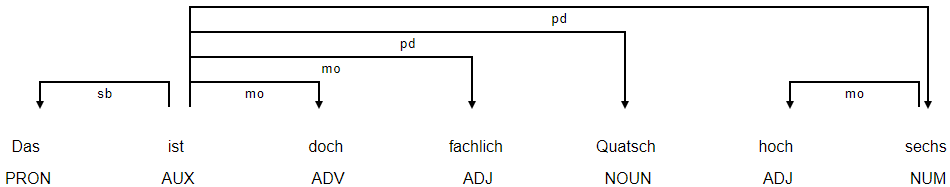
\includegraphics[width=1\textwidth]{chapters/04-Sentiment-Analyse/steffi.png}}
\caption{Visualisierung der Wortabhängigkeiten (Zitat von Steffi Lemke MdB, 208. Sitzung, 10.02.2021)}
\label{steffi}
\end{figure}

\subsection{Negations-Erkennung}
\label{neg-erkennung}
Negation, also Ablehnung, Verneinung oder Aufhebung, hat einen erheblichen Einfluss auf das Ergebnis und damit die Korrektheit der Sentimentanalyse, weshalb in dieser Arbeit ein besonderes Augenmerk auf ihre Erkennung gelegt wurde. 
In \textit{Negation Modeling for German Polarity Classification} \cite{g3_wieg} präsentieren Forscher der Universität des Saarlandes und des Leibniz-Institut für Deutsche Sprache hierfür einen regelbasierten Ansatz. 

Sie definieren unterschiedliche Negationstypen und ihre jeweilige Reichweite. 
So beeinflussen etwa negierende Adverbien oder Indefinitpronomen wie \textit{nie} den gesamten Satz, wohingegen das Partikel \textit{nicht} lediglich seinen Vorgänger negiert.  
Die Tabelle \ref{g3tab1} führt alle in dieser Arbeit implementierten Negationsregeln auf. 
Die Nutzung eines Abhängigkeitsbaumes, wie von \mintinline{latex}{spaCy} ermittelt, ist dabei unerlässlich. 
Denn wie schon im vorherigen Kapitel angesprochen, ist etwa mit dem Vorgänger eines Wortes nicht das in der Satzabfolge voranstehende Wort gemeint, sondern vielmehr der semantische Regent. 

\begin{table}[htbp]
\caption{Implementierte Negations-Regeln aus \cite{g3_wieg}}
\begin{center}
\begin{tabular}{| c | c | c |}
\hline
\textbf{Negationstyp} & \textbf{Reichweite} & \textbf{Beispielworte} \\ \hline
Partikel & Vorgänger (Regent) & nicht \\ \hline
Präpositionen & Nachfolger (Dependent) & ohne, gegen \\ \hline
Adverbien, & Satz & nie, kein, kaum \\
Indefinitpronomen &  &  \\ \hline
Nomen & Genitiv,& Abschaffung, \\
 & Präpositionalobjekt & Zerstörung \\ \hline
Verben & Objekt, Subjekt & enden, sinken, lindern \\
\hline
\end{tabular}
\label{g3tab1}
\end{center}
\end{table}

Angemerkt sei an dieser Stelle, dass es nicht möglich war, alle Regeln aus \cite{g3_wieg} zu implementieren, da der von den Forschern genutzte Dependency-Parser umfangreichere Ergebnisse liefert, als jener von \mintinline{latex}{spaCy}. 

Eine Liste mit Negationsworten und dem jeweiligen Negationstyp wurde \cite{g3_polcla} entnommen und ist ebenfalls über die Klasse \mintinline{latex}{Lexicon} zugreifbar. 
Die Klasse stellt ein \mintinline{latex}{Dictionary} bereit, in welchem die Schlüssel die Negationsworte und die Werte eine Liste der Reichweiten sind. 

Wenn in einem Text ein Negationswort auftritt, werden alle implementierten Regeln geprüft. 
Sollte es zu einem Treffer kommen, etwa wenn das Wort \textit{nicht} auftritt (siehe Abb. \ref{brandner}) und es einen Vorgänger gibt, werden alle Worte in Reichweite des Negationswortes negiert. 
Dies geschieht, indem für die jeweiligen Worte, welche wie in \ref{g3textv} beschrieben \mintinline{latex}{Token}-Objekte sind, ein eigenes Attribut mit der Bezeichnung \mintinline{latex}{negated} auf \mintinline{latex}{True} gesetzt wird. 
In der Polaritätsberechnung wird wortweise auf dieses Attribut geprüft und die Wort-Polarität bei einer Negierung mit -1 multipliziert. 

\begin{figure}[htb]
\centerline{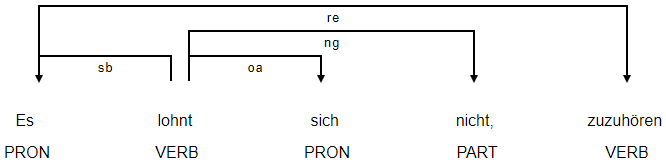
\includegraphics[width=1\textwidth]{chapters/04-Sentiment-Analyse/brandner.png}}
\caption{Beispielsatz mit Patikel-Negation (Zitat von Stephan Brandner MdB, 207. Sitzung, 29.01.2021)}
\label{brandner}
\end{figure}

\subsection{Verstärkungs-Erkennung}
\label{ver-erkennung}
Als \textit{Verstärker} werden sog. Gradpartikel (z.B. sehr, besonders, viel) verstanden, welche direkt vor Adjektiven oder Adverbien in einem Satz auftreten. 
Sie verstärken ihren Nachfolger, was wiederum in der Polaritätsberechnung berücksichtigt werden soll. 

Aus diesem Grund wird eine Liste mit verstärkenden Gradpartikeln, welche ebenfalls aus \cite{g3_polcla} bezogen werden, eingelesen und über die \mintinline{latex}{Lexicon} Klasse bereitgestellt. 

Ebenso wie in Kapitel \ref{neg-erkennung} bereits für die Negation beschrieben, wird ein eigenes Attribut zur Signalisierung einer Verstärkung definiert und im entsprechenden Fall auf True gesetzt. 
Bei der Polaritätsberechnung wird bei einer erkannten Verstärkung die Wort-Polarität mit 1,5 multipliziert \cite{g3_sentia}. 

In Abbildung \ref{hessel} wird ein Beispiel für das Auftreten eines verstärkenden Gradpartikels gegeben. 
Hier verstärkt das Wort \textit{sehr} das negative Wort \textit{spät}, womit die errechnete Polarität stärker negativ ausfällt als ohne die Verstärkungs-Erkennung. 

\begin{figure}[htb]
\centerline{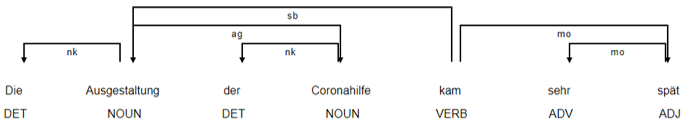
\includegraphics[width=1\textwidth]{chapters/04-Sentiment-Analyse/hessel.png}}
\caption{Beispielsatz mit Gradpartikel-Verstärkung (Zitat von Katja Hessel MdB, 206. Sitzung, 28.01.2021)}
\label{hessel}
\end{figure}

\subsection{Polaritätsberechnung}
\label{polberechnung}
Für die abschließende Berechnung der Polarität sind verschiedene Formeln denkbar. 
Sie sollten anhand von Textcharakteristika wie z.B. der Satz- oder Textlänge gewählt werden. 

Bei der Verwendung einer satzbasierten Polaritätsberechnung, bei welcher alle Polaritäten erst addiert und die Summe anschließend durch die Anzahl der Worte dividiert wird, kann ein unerwünschtes Phänomen auftreten: 
Längere Sätze erhaltenen ein stärker polarisiertes Ergebnis als vergleichbare kurze Sätze. 

Dies ist mit einer im Schnitt höheren Dichte an Worten mit Polaritäts-Wert in längeren Sätzen zu erklären. 
Um diesem Problem entgegen zu wirken, wurde in dieser Arbeit eine Min-Max-Skalierung (siehe Formeln 1 - 3) auf Dokumentebene implementiert \cite{g3_sentia}. 

Die Entscheidung, diese Normalisierung anhand der Länge des gesamten Textes durchzuführen, wurde aufgrund der Charakteristika der zu analysierenden Interaktionen getroffen. 
Denn diese bestehen zu einem überwiegenden Teil aus einem einzelnen Satz von jedoch sehr unterschiedlicher Länge. 

\begin{align}
p' &= \frac{ p + 1 }{ text.len + 1 } \text{ für p $>$ 0}\\
p' &= \frac{ p - 1 }{ text.len + 1 } \text{ für p $<$ 0}\\
p' &= p \text{ für p $=$ 0}
\end{align}

\section{Evaluierung}
\subsection{Sprache im Bundestag}
\label{sprachebundestag}
Während der Entwicklung dieser Arbeit und den regelmäßig angestellten Zwischentests wurde ersichtlich, dass sich die Sprache im Bundestag etwa von jener in sozialen Netzwerken oder Produktbewertungen unterschiedet. 
Ein Interaktionstext setzt sich sowohl aus einzelnen, langen und komplexe Sätze zusammen, als auch aus einzelnen Ausrufen wie \textit{\glqq eieiei!\grqq} zusammen. 

Aus diesem Grund wurde die in \ref{polberechnung} beschriebene Normalisierung verwendet, da herkömmliche Berechnungsformeln zunächst widersprüchliche Ergebnisse lieferten. 
Gleichzeitig verbesserte die manuelle Durchsicht der häufigsten 15.000 Worte und Anfertigung einer eigenen Bundestags-Wortliste das Ergebnis deutlich. 
Viele der regelmäßig in Bundestagssitzungen verwendeten Worte gehören zur \textit{Politik-Domäne} und treten deshalb nicht in den Quell-Wortlisten auf. 
Hier wird erwartet, dass eine noch umfangreichere Bundestags-Wortliste einen weiteren positiven Einfluss auf das Endergebnis hätte. 
Aus Zeit- sowie Kompetenzgründen wurde diese Liste jedoch nicht erweitert. 

\subsection{Ironie und Sarkasmus}
Ebenso wie die im vorherigen besprochene \textit{Politiksprache}, treten auch Ironie und Sarkasmus vermehrt in den Sitzungen des Bundestages auf. 
Einfach umrissen, handelt es sich dabei um ein Stilmittel, bei dem das Gegenteil vom Gesagten gemeint ist. 
Sarkasmus ist dabei eine verstärkte Form der Ironie und kann auch als ein Angriff verstanden werden. 

Selbst für den menschlichen Leser ist allein am geschriebenen Text nicht immer ersichtlich, ob eine Aussage ironisch gemeint ist. 
Vielmehr wird für die richtige Deutung die Stimmlage, Gestik und Mimik der sprechenden Person benötigt. 

Ironie und Sarkasmus könne also erst recht nicht mit dem in dieser Arbeit verwendeten Wortlisten-Ansatz erkannt werden, womit ein unbekannter Teil der Interaktionen im Ergebnis die falsche Polarität besitzt. 
Gleichwohl gibt es Ansätze aus dem Bereich des maschinellen Lernens, welche dieses Problem behandeln. 
Jedoch setzen diese einen entsprechend annotierten Korpus vorraus und stammen zudem aus dem Bereich der sozialen Netzwerke, in welchen etwa mit \textit{Hashtags} die Ironie bereits vom Autor markiert wurde. 

\subsection{Fazit}
Trotzt der soeben beschriebenen Fehlerquellen, wurde dennoch ein gelungenes Ergebnis erzielt: 
Es wurde ein solider und erweiterbarer Algorithmus zur Sentimentananlyse von Texten geschaffen, welcher auf den bekanntesten Bibliotheken und Techniken der Textverarbeitung beruht. 
Dieser kann als Basis für weitere Anstrengungen bei der Sentimentanalyse von politischen Texten dienen. 

Eine Deutung der bisherigen Ergebnisse durch Politikwissenschaftler oder anderweitig in diesem Bereich kompetente Personen wird dabei empfohlen, um die beschriebenen Schwachstellen entsprechend zu behandeln oder neue zu identifizieren. 

Der Programmcode ist zudem vollständig und abgesichert in die Projektpipeline eingebunden. 
Er erweitert seine Ergebnis-Datenbank automatisch um neue Sitzungen und benachrichtigt anschließend nachfolgende Gruppen. 

\section{Grundlagen}\label{sec:07_02_grundlagen}
\section{Anforderungsanalyse und Konzept}\label{sec:08_03_anforderungen_konzept}


\section{Zusammenfassung und Ausblick}\label{sec:07_05_zusammenfassung}

\chapter{Analyse der Interaktion zwischen Abgeordneten}
\section{Einleitung}
Der Begriff \textit{Sentiment} stammt vom lateinischen Wort \textit{sentimentum} ab und bedeutet Empfindung oder Stimmung. 
In der Sentimentanalyse geht es um die Bestimmung eben jener Stimmung einer Meinungsäußerung. 
Anwendung findet sie etwa bei Produktbewertungen oder Beiträgen in sozialen Netzwerken. 
Die Stimmung wird durch die sog. Polarität beschrieben und kann positiv, negativ oder neutral ausfallen. 
Im Text-Mining wird sie im Intervall $\interval{-1}{1} = \{x \in \mathbb{R} | -1 \leq x \leq 1\}$ angegeben, wobei -1 sehr negativ, 1 sehr positiv und 0 neutral bedeuten. 

Grundlegend ist die maschinelle Sentimentanalyse entweder Wortlisten- oder Modell-basiert. 
Der Wortlisten-Ansatz kann als eine Sammlung von Worten und ihrer Polaritäten verstanden werden, anhand welcher die Stimmung berechnet wird. 
Dieser Ansatz wird weiter im Kapitel \ref{wortliste} beschrieben, da er in dieser Arbeit verwendet wurde. 

Bei der Modell-basierten Sentimentanalyse wird ein annotierter Satz-Korpus für das Trainieren einer künstlichen Intelligenz vorausgesetzt. 
Etwa für Twitter-Beiträge stehen solche Korpusse oder auch bereits trainierte Modelle zur Verfügung. 
Jedoch ist bei der Verwendung zur Analyse der Sitzungsprotokolle des Bundestages nicht mit zufriedenstellenden Ergebnissen zu rechnen, da sich verwendete Worte und Text- bzw. Satzbau zwischen diesen Domänen deutlich unterscheiden. 
Eine weitere Erläuterung zur Sprache im Bundestag wird in Kapitel \ref{sprachebundestag} gegeben. 

Ebenfalls werden die Komponenten zur Teilnahme an der Verarbeitungspipeline des Gesamtprojektes im nachfolgenden Kapitel \ref{g3daten} beschrieben. 

\section{Datenaustausch}
\label{g3daten}
\subsection{Datenimport}
Für das Erhalten von Daten wurde eine Methode implementiert, welche durch Angabe einer Sitzungs-ID die entsprechende Sitzung vom REST-API von Gruppe 2 abfragen kann. 
Diese Methode gibt jede Sitzung weiter an die in Kapitel \ref{g3textv} beschriebene Textverarbeitung und das Ergebnis schließlich an den in Kapitel \ref{g3export} beschriebenen Export-Code. 

Die Methode wird für zwei Fälle verwendet: 
Beim Normalfall sendet die Gruppe 2 eine Benachrichtigung mit einer Liste aller neuen Sitzungs-IDs an das REST-API im Code dieser Arbeit. 
Das REST-API wurde mit der Bibliothek \mintinline{latex}{Flask} \cite{g3_flask} entwickelt und besteht aus einer POST-Schnittstelle, welche auf dem von der HTW bereitgestelltem Server unter \textit{/notify} erreichbar ist. 

Das API wurde unter Zuhilfenahme von \mintinline{latex}{Flask.Blueprints} \cite{g3_flaskbp} entwickelt und wird von einem \mintinline{latex}{Waitress}-Webserver \cite{g3_waitress} bereitgestellt. 
Für jede Anfrage wird geprüft, ob Content-Type und Payload dem erwarteten JSON-Daten entsprechen. 
Sollte dies nicht der Fall sein, wird eine entsprechende Rückmeldung an den Sender zurückgegeben. 
Für jede erhaltene Sitzungs-ID wird die eingangs beschriebene Methode aufgerufen. 

Der zweite Fall wurde vor allem im Rahmen der voranschreitenden Entwicklung bei den in der Projektpipeline voranstehenden Gruppen verwendet. 
Statt auf eine Benachrichtigung zum Anstoßen des Datenimports zu warten, werden stattdessen alle Sitzungs-IDs vom REST-API der Gruppe 2 abgefragt und jede Sitzung vollständig neu importiert. 
Dieses Vorgehen hat den Vorteil, dass eventuell durch Arbeit am Code verpasste Benachrichtigungen nachgeholt werden und gleichzeitig Änderungen an den Daten übernommen werden können. 

\subsection{Datenexport}
\label{g3export}
Statt Arbeit in ein umfangreiches REST-API für die nachfolgenden Gruppen zu stecken, wurde für diese Arbeit ein reiner MongoDB-Ansatz verwendet. 
Auf dem zur Verfügung stehenden HTW-Server wurde dafür eine MongoDB Instanz aufgesetzt, welche nur aus dem HTW-Netz erreichbar und zudem nur mit Authentifizierung zugreifbar ist. 
Jede Sitzung ist hier als eine eigene Collection persistiert. 
Sobald neue Sitzungen importiert und verarbeitet wurden, werden diese zunächst mit dem MongoDB-Treiber \mintinline{latex}{PyMongo} \cite{g3_mongodb} in die Datenbank geschrieben. 
Anschließend werden die nachfolgenden Gruppen mit einem POST and die jeweilige REST-Schnittstelle benachrichtigt, dass neue Daten vorliegen. 
Diese greifen dann mit den zuvor versendeten Zugangsdaten direkt auf die Datenbank zu. 

Mit diesem Vorgehen konnte die Komplexität beim Zugriff auf die Ergebnis-Daten gesenkt werden, da es für nahezu alle gängigen Programmiersprachen einen intuitiven MongoDB-Treiber gibt. 

\section{Wortliste}
\label{wortliste}
Wie bereits in der Einleitung beschrieben, handelt es sich bei Wortlisten in der Sentimentanalyse um eine Liste von Worten und ihrer jeweiligen Polarität. 
Bei der Analyse eines Textes wird wortweise ein Abgleich mit dieser Liste durchgeführt und die Wort-Polarität bei einer Übereinstimmung für die Berechnung des Sentiments verwendet. 
Unterschiedliche Berechnungsformeln sind dabei denkbar und werden in Kapitel \ref{polberechnung} weiter besprochen. 
Für diese Arbeit wurden Wortlisten verschiedener Institutionen kombiniert und anschließend mit Synonymen erweitert. 
Ebenfalls wurde eine eigene Bundestags-Wortliste erstellt. 

Die Interest Group on German Sentiment Analysis (IGGSA) stellt eine umfangreiche Liste an Publikationen und Ressourcen zu Sentimentanalysen in der deutschen Sprache zur Verfügung \cite{g3_iggsa}. 
Hier wurden alle Referenzen auf die in dieser Arbeit verwendeten Quell-Wortlisten gesammelt. 
Für die Zusammenführung dieser Wortlisten wurden zunächst zwei Herangehensweisen evaluiert: 
Zum einen war die Erstellung eines eigenständigen Codes denkbar, welcher einmalig die Daten aus allen Quellen einliest, zusammenfasst und eine Ergebnis-Datei ausgibt. 
Diese Datei wäre eine Ressource für den eigentlichen Analyse-Code. 
Zum anderen könnte die soeben beschriebene Funktionalität jedoch auch direkt im Analyse-Code integriert und bei jedem Programmstart ausgeführt werden. 
Die kombinierte Wortliste würde somit nicht auf die Festplatte geschrieben, sondern im Arbeitsspeicher verbleiben, solange der Analyse-Code läuft. 
Wenngleich der zuerst beschriebene Ansatz offensichtlich weniger Rechenzeitaufwändig ist, wurde für diese Arbeit der zweite Ansatz gewählt. 
Dies wird vor allem mit Rechtsunsicherheiten bei der Arbeit mit den verschiedenen Lizenzen der Quelldateien begründet. 
Gleichzeitig arbeitet der Analyse-Code damit jederzeit mit dem aktuellen Stand der Quell-Wortlisten. 
Das Aufbauen der Wortliste dauert wenige Minuten. 

Für diese Arbeit wurden die folgenden Quell-Wortlisten verwendet: 

\begin{itemize}
\item \textit{SentimentWortschatz} (SentiWS) aus \glqq SentiWS - a Publicly Available German-language Resource for Sentiment Analysis\grqq (Universität Leipzig) \cite{g3_sentiws}
\item \textit{Multi-Domain Sentiment Lexicon for German} (Hochschule Darmstadt) \cite{g3_opm}
\item \textit{German Polarity Lexicon} aus \glqq Evaluation and extension of a polarity lexicon for German\grqq (Universität Zürich) \cite{g3_polcla}
\item \textit{morphcomp} aus \glqq Evaluating the morphological compositionality of pola-rity\grqq (Leibniz-Institut für Deutsche Sprache, Universität des Saarlandes) \cite{g3_morphcomp}
\end{itemize}

Aus diesen Quellen ergibt sich eine Wortliste mit etwa 14.000 einzigartigen Worten. 
Die Worte werden dabei mit der in Kapitel \ref{g3textv} beschriebenen Textverarbeitungspipeline lemmatisiert, also auf die Grundform zurückgeführt. 
Bei Überschneidungen wird ein Mittelwert über alle Polaritäts-Werte eines Wortes gebildet. 

Mithilfe des \textit{Open German WordNet} (OdeNet) \cite{g3_odenet} werden zu jedem Wort Synonyme gesammelt und ebenfalls der Wortliste hinzugefügt. 
Der Zugriff auf OdeNet geschieht dabei mit der python Bibliothek \mintinline{latex}{WN} \cite{g3_wn}. 
Die Verwendung dieser Bibliothek ist trivial, weshalb an dieser Stelle keine weitere Erläuterung gegeben wird. 
Die Wortliste wird durch das Hinzufügen von Synonymen um weitere rund 2.000 Worte erweitert. 

Wie bereits in der Einleitung erwähnt, wurde zudem eine eigene Bundes-tags-Wortliste erstellt. 
Hierzu wurden die 15.000 am häufigsten in den Sitzungsprotokollen vorkommenden Worte erfasst und analysiert. 
Dabei wurden jedoch nur jene Worte betrachtet, welche nicht bereits in der kombinierten Wortliste vorkommen. 
Ausgewählt wurden nur eindeutig positive oder negative Worte wie \textit{angemessen}, \textit{Bullshit}, \textit{Fehlentscheidung}, \textit{Milchmädchenrechnung}, \textit{Realitätsverweigerung}, \textit{Totalausfall} oder \textit{Verunglimpfung}. 
Insgesamt umfasst die Bundestags-Wortliste 217 Worte. 

Im Code wird der Zugriff auf die Wortliste mit der zentralen Klasse \mintinline{latex}{Lexicon} realisiert. 
Bei der Instanziierung der Klasse werden, wie im Vorherigen beschrieben, alle Wortlisten gesammelt, zusammengeführt und erweitert. 
Anschließend stellt die Klasse ein \mintinline{latex}{Dictionary} bereit, in welchem die Schlüssel die Worte und die Werte die Wort-Polarität angeben. 

\section{Textverarbeitung}
\label{g3textv}
Für die Textverarbeitung nutzt der Code dieser Arbeit vollständig die Funktionalitäten und Strukturen von \mintinline{latex}{spaCy} \cite{g3_spacy}. 
Die \mintinline{latex}{spaCy} Bibliothek stellt eine Textverarbeitungspipeline bereit, welche mithilfe eines vortrainierten Modells funktioniert. 
Für die deutsche Sprache wurde ein solches Modell mit dem TIGER Korpus der Universität Stuttgart trainiert. 
Der Korpus umfasst ca. 50.000 Sätze aus Texten der Frankfurter Rundschau. 
Die \mintinline{latex}{spaCy}-Pipeline besteht aus den folgenden Komponenten: 

\begin{itemize}
\item Tokenisierung (Text- und Satzzerteilung)
\item POS-Tagging (Wortartenerkennung)
\item Dependency-Parsing (Wortabhängigkeitenerkennung)
\item Lemmatisierung (Wortgrundformermittlung)
\item Entity-Recognition (Eigennamenerkennung)
\end{itemize}

Das Ergebnis der Pipeline ist ein \mintinline{latex}{Doc}-Objekt, welches das Ergebnis des gesamten in die Pipeline gegebenen Textes umfasst. 
Einzelne Sätze innerhalb des \mintinline{latex}{Doc}-Objektes werden mit \mintinline{latex}{Span}-Objekten beschrieben und einzelne Worte mit \mintinline{latex}{Token}-Objekten. 
Die Objekttypen besitzen jeweils eigene Methoden und Erweiterungsmöglichkeiten in Form von sog. \textit{extension attributes}. 

Sehr einfach und gleichzeitig umfangreich kann die \mintinline{latex}{spaCy}-Pipeline an die eigenen Bedürfnisse angepasst werden. 
So wurde die Berechnung des Sentiments eines Textes direkt an die Komponenten der Standart-Pipeline angehängt. 
Logisch unterteilt sich diese in die Komponenten:

\begin{itemize}
\item Negations-Erkennung (siehe \ref{neg-erkennung})
\item Verstärkungs-Erkennung (siehe \ref{ver-erkennung})
\item Polaritätsberechnung (siehe \ref{polberechnung})
\end{itemize}

Basis für das nachfolgende Kapitel \ref{neg-erkennung} ist dabei das Ergebnis des Depen-dency-Parsers von \mintinline{latex}{spaCy}. 
Dieser bestimmt die Abhängigkeiten zwischen den einzelnen Elementen eines Satzes. 
Diese Funktion gehört dem Themenbereich der Dependenzgrammatik an, in welcher gerichtete Beziehungen zwischen den Worten eines Satzes beschreibt werden. 
Ein Wort kann einen Vorgänger (Regent) und mehrere Nachfolger (Dependenten) besitzen. 
Die Gesamtheit der Beziehungen eines Satzes wird auch Abhängigkeitsbaum genannt. 

Zur Verdeutlichung soll die Abbildung \ref{steffi} dienen, welche mithilfe von \mintinline{latex}{spaCy.displaCy} erstellt wurde. 
Zu sehen ist hier der Abhängigkeitsbaum des Satzes \textit{\glqq Das ist doch fachlich Quatsch hoch sechs!\grqq}. 
An den gerichteten Kanten befindet sich die Angabe des Satzgliedes, unterhalb der Worte die Angabe der Wortart. 

\begin{figure}[htb]
\centerline{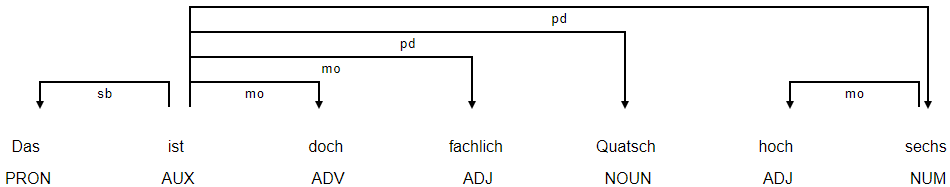
\includegraphics[width=1\textwidth]{chapters/04-Sentiment-Analyse/steffi.png}}
\caption{Visualisierung der Wortabhängigkeiten (Zitat von Steffi Lemke MdB, 208. Sitzung, 10.02.2021)}
\label{steffi}
\end{figure}

\subsection{Negations-Erkennung}
\label{neg-erkennung}
Negation, also Ablehnung, Verneinung oder Aufhebung, hat einen erheblichen Einfluss auf das Ergebnis und damit die Korrektheit der Sentimentanalyse, weshalb in dieser Arbeit ein besonderes Augenmerk auf ihre Erkennung gelegt wurde. 
In \textit{Negation Modeling for German Polarity Classification} \cite{g3_wieg} präsentieren Forscher der Universität des Saarlandes und des Leibniz-Institut für Deutsche Sprache hierfür einen regelbasierten Ansatz. 

Sie definieren unterschiedliche Negationstypen und ihre jeweilige Reichweite. 
So beeinflussen etwa negierende Adverbien oder Indefinitpronomen wie \textit{nie} den gesamten Satz, wohingegen das Partikel \textit{nicht} lediglich seinen Vorgänger negiert.  
Die Tabelle \ref{g3tab1} führt alle in dieser Arbeit implementierten Negationsregeln auf. 
Die Nutzung eines Abhängigkeitsbaumes, wie von \mintinline{latex}{spaCy} ermittelt, ist dabei unerlässlich. 
Denn wie schon im vorherigen Kapitel angesprochen, ist etwa mit dem Vorgänger eines Wortes nicht das in der Satzabfolge voranstehende Wort gemeint, sondern vielmehr der semantische Regent. 

\begin{table}[htbp]
\caption{Implementierte Negations-Regeln aus \cite{g3_wieg}}
\begin{center}
\begin{tabular}{| c | c | c |}
\hline
\textbf{Negationstyp} & \textbf{Reichweite} & \textbf{Beispielworte} \\ \hline
Partikel & Vorgänger (Regent) & nicht \\ \hline
Präpositionen & Nachfolger (Dependent) & ohne, gegen \\ \hline
Adverbien, & Satz & nie, kein, kaum \\
Indefinitpronomen &  &  \\ \hline
Nomen & Genitiv,& Abschaffung, \\
 & Präpositionalobjekt & Zerstörung \\ \hline
Verben & Objekt, Subjekt & enden, sinken, lindern \\
\hline
\end{tabular}
\label{g3tab1}
\end{center}
\end{table}

Angemerkt sei an dieser Stelle, dass es nicht möglich war, alle Regeln aus \cite{g3_wieg} zu implementieren, da der von den Forschern genutzte Dependency-Parser umfangreichere Ergebnisse liefert, als jener von \mintinline{latex}{spaCy}. 

Eine Liste mit Negationsworten und dem jeweiligen Negationstyp wurde \cite{g3_polcla} entnommen und ist ebenfalls über die Klasse \mintinline{latex}{Lexicon} zugreifbar. 
Die Klasse stellt ein \mintinline{latex}{Dictionary} bereit, in welchem die Schlüssel die Negationsworte und die Werte eine Liste der Reichweiten sind. 

Wenn in einem Text ein Negationswort auftritt, werden alle implementierten Regeln geprüft. 
Sollte es zu einem Treffer kommen, etwa wenn das Wort \textit{nicht} auftritt (siehe Abb. \ref{brandner}) und es einen Vorgänger gibt, werden alle Worte in Reichweite des Negationswortes negiert. 
Dies geschieht, indem für die jeweiligen Worte, welche wie in \ref{g3textv} beschrieben \mintinline{latex}{Token}-Objekte sind, ein eigenes Attribut mit der Bezeichnung \mintinline{latex}{negated} auf \mintinline{latex}{True} gesetzt wird. 
In der Polaritätsberechnung wird wortweise auf dieses Attribut geprüft und die Wort-Polarität bei einer Negierung mit -1 multipliziert. 

\begin{figure}[htb]
\centerline{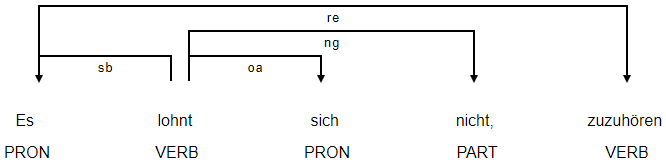
\includegraphics[width=1\textwidth]{chapters/04-Sentiment-Analyse/brandner.png}}
\caption{Beispielsatz mit Patikel-Negation (Zitat von Stephan Brandner MdB, 207. Sitzung, 29.01.2021)}
\label{brandner}
\end{figure}

\subsection{Verstärkungs-Erkennung}
\label{ver-erkennung}
Als \textit{Verstärker} werden sog. Gradpartikel (z.B. sehr, besonders, viel) verstanden, welche direkt vor Adjektiven oder Adverbien in einem Satz auftreten. 
Sie verstärken ihren Nachfolger, was wiederum in der Polaritätsberechnung berücksichtigt werden soll. 

Aus diesem Grund wird eine Liste mit verstärkenden Gradpartikeln, welche ebenfalls aus \cite{g3_polcla} bezogen werden, eingelesen und über die \mintinline{latex}{Lexicon} Klasse bereitgestellt. 

Ebenso wie in Kapitel \ref{neg-erkennung} bereits für die Negation beschrieben, wird ein eigenes Attribut zur Signalisierung einer Verstärkung definiert und im entsprechenden Fall auf True gesetzt. 
Bei der Polaritätsberechnung wird bei einer erkannten Verstärkung die Wort-Polarität mit 1,5 multipliziert \cite{g3_sentia}. 

In Abbildung \ref{hessel} wird ein Beispiel für das Auftreten eines verstärkenden Gradpartikels gegeben. 
Hier verstärkt das Wort \textit{sehr} das negative Wort \textit{spät}, womit die errechnete Polarität stärker negativ ausfällt als ohne die Verstärkungs-Erkennung. 

\begin{figure}[htb]
\centerline{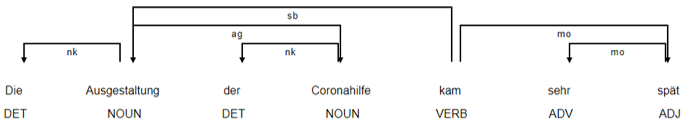
\includegraphics[width=1\textwidth]{chapters/04-Sentiment-Analyse/hessel.png}}
\caption{Beispielsatz mit Gradpartikel-Verstärkung (Zitat von Katja Hessel MdB, 206. Sitzung, 28.01.2021)}
\label{hessel}
\end{figure}

\subsection{Polaritätsberechnung}
\label{polberechnung}
Für die abschließende Berechnung der Polarität sind verschiedene Formeln denkbar. 
Sie sollten anhand von Textcharakteristika wie z.B. der Satz- oder Textlänge gewählt werden. 

Bei der Verwendung einer satzbasierten Polaritätsberechnung, bei welcher alle Polaritäten erst addiert und die Summe anschließend durch die Anzahl der Worte dividiert wird, kann ein unerwünschtes Phänomen auftreten: 
Längere Sätze erhaltenen ein stärker polarisiertes Ergebnis als vergleichbare kurze Sätze. 

Dies ist mit einer im Schnitt höheren Dichte an Worten mit Polaritäts-Wert in längeren Sätzen zu erklären. 
Um diesem Problem entgegen zu wirken, wurde in dieser Arbeit eine Min-Max-Skalierung (siehe Formeln 1 - 3) auf Dokumentebene implementiert \cite{g3_sentia}. 

Die Entscheidung, diese Normalisierung anhand der Länge des gesamten Textes durchzuführen, wurde aufgrund der Charakteristika der zu analysierenden Interaktionen getroffen. 
Denn diese bestehen zu einem überwiegenden Teil aus einem einzelnen Satz von jedoch sehr unterschiedlicher Länge. 

\begin{align}
p' &= \frac{ p + 1 }{ text.len + 1 } \text{ für p $>$ 0}\\
p' &= \frac{ p - 1 }{ text.len + 1 } \text{ für p $<$ 0}\\
p' &= p \text{ für p $=$ 0}
\end{align}

\section{Evaluierung}
\subsection{Sprache im Bundestag}
\label{sprachebundestag}
Während der Entwicklung dieser Arbeit und den regelmäßig angestellten Zwischentests wurde ersichtlich, dass sich die Sprache im Bundestag etwa von jener in sozialen Netzwerken oder Produktbewertungen unterschiedet. 
Ein Interaktionstext setzt sich sowohl aus einzelnen, langen und komplexe Sätze zusammen, als auch aus einzelnen Ausrufen wie \textit{\glqq eieiei!\grqq} zusammen. 

Aus diesem Grund wurde die in \ref{polberechnung} beschriebene Normalisierung verwendet, da herkömmliche Berechnungsformeln zunächst widersprüchliche Ergebnisse lieferten. 
Gleichzeitig verbesserte die manuelle Durchsicht der häufigsten 15.000 Worte und Anfertigung einer eigenen Bundestags-Wortliste das Ergebnis deutlich. 
Viele der regelmäßig in Bundestagssitzungen verwendeten Worte gehören zur \textit{Politik-Domäne} und treten deshalb nicht in den Quell-Wortlisten auf. 
Hier wird erwartet, dass eine noch umfangreichere Bundestags-Wortliste einen weiteren positiven Einfluss auf das Endergebnis hätte. 
Aus Zeit- sowie Kompetenzgründen wurde diese Liste jedoch nicht erweitert. 

\subsection{Ironie und Sarkasmus}
Ebenso wie die im vorherigen besprochene \textit{Politiksprache}, treten auch Ironie und Sarkasmus vermehrt in den Sitzungen des Bundestages auf. 
Einfach umrissen, handelt es sich dabei um ein Stilmittel, bei dem das Gegenteil vom Gesagten gemeint ist. 
Sarkasmus ist dabei eine verstärkte Form der Ironie und kann auch als ein Angriff verstanden werden. 

Selbst für den menschlichen Leser ist allein am geschriebenen Text nicht immer ersichtlich, ob eine Aussage ironisch gemeint ist. 
Vielmehr wird für die richtige Deutung die Stimmlage, Gestik und Mimik der sprechenden Person benötigt. 

Ironie und Sarkasmus könne also erst recht nicht mit dem in dieser Arbeit verwendeten Wortlisten-Ansatz erkannt werden, womit ein unbekannter Teil der Interaktionen im Ergebnis die falsche Polarität besitzt. 
Gleichwohl gibt es Ansätze aus dem Bereich des maschinellen Lernens, welche dieses Problem behandeln. 
Jedoch setzen diese einen entsprechend annotierten Korpus vorraus und stammen zudem aus dem Bereich der sozialen Netzwerke, in welchen etwa mit \textit{Hashtags} die Ironie bereits vom Autor markiert wurde. 

\subsection{Fazit}
Trotzt der soeben beschriebenen Fehlerquellen, wurde dennoch ein gelungenes Ergebnis erzielt: 
Es wurde ein solider und erweiterbarer Algorithmus zur Sentimentananlyse von Texten geschaffen, welcher auf den bekanntesten Bibliotheken und Techniken der Textverarbeitung beruht. 
Dieser kann als Basis für weitere Anstrengungen bei der Sentimentanalyse von politischen Texten dienen. 

Eine Deutung der bisherigen Ergebnisse durch Politikwissenschaftler oder anderweitig in diesem Bereich kompetente Personen wird dabei empfohlen, um die beschriebenen Schwachstellen entsprechend zu behandeln oder neue zu identifizieren. 

Der Programmcode ist zudem vollständig und abgesichert in die Projektpipeline eingebunden. 
Er erweitert seine Ergebnis-Datenbank automatisch um neue Sitzungen und benachrichtigt anschließend nachfolgende Gruppen. 

\section{Grundlagen}\label{sec:07_02_grundlagen}
\section{Anforderungsanalyse und Konzept}\label{sec:08_03_anforderungen_konzept}


\section{Zusammenfassung und Ausblick}\label{sec:07_05_zusammenfassung}

\chapter{Analyse der Interaktion zwischen Fraktionen}
\section{Einleitung}
Der Begriff \textit{Sentiment} stammt vom lateinischen Wort \textit{sentimentum} ab und bedeutet Empfindung oder Stimmung. 
In der Sentimentanalyse geht es um die Bestimmung eben jener Stimmung einer Meinungsäußerung. 
Anwendung findet sie etwa bei Produktbewertungen oder Beiträgen in sozialen Netzwerken. 
Die Stimmung wird durch die sog. Polarität beschrieben und kann positiv, negativ oder neutral ausfallen. 
Im Text-Mining wird sie im Intervall $\interval{-1}{1} = \{x \in \mathbb{R} | -1 \leq x \leq 1\}$ angegeben, wobei -1 sehr negativ, 1 sehr positiv und 0 neutral bedeuten. 

Grundlegend ist die maschinelle Sentimentanalyse entweder Wortlisten- oder Modell-basiert. 
Der Wortlisten-Ansatz kann als eine Sammlung von Worten und ihrer Polaritäten verstanden werden, anhand welcher die Stimmung berechnet wird. 
Dieser Ansatz wird weiter im Kapitel \ref{wortliste} beschrieben, da er in dieser Arbeit verwendet wurde. 

Bei der Modell-basierten Sentimentanalyse wird ein annotierter Satz-Korpus für das Trainieren einer künstlichen Intelligenz vorausgesetzt. 
Etwa für Twitter-Beiträge stehen solche Korpusse oder auch bereits trainierte Modelle zur Verfügung. 
Jedoch ist bei der Verwendung zur Analyse der Sitzungsprotokolle des Bundestages nicht mit zufriedenstellenden Ergebnissen zu rechnen, da sich verwendete Worte und Text- bzw. Satzbau zwischen diesen Domänen deutlich unterscheiden. 
Eine weitere Erläuterung zur Sprache im Bundestag wird in Kapitel \ref{sprachebundestag} gegeben. 

Ebenfalls werden die Komponenten zur Teilnahme an der Verarbeitungspipeline des Gesamtprojektes im nachfolgenden Kapitel \ref{g3daten} beschrieben. 

\section{Datenaustausch}
\label{g3daten}
\subsection{Datenimport}
Für das Erhalten von Daten wurde eine Methode implementiert, welche durch Angabe einer Sitzungs-ID die entsprechende Sitzung vom REST-API von Gruppe 2 abfragen kann. 
Diese Methode gibt jede Sitzung weiter an die in Kapitel \ref{g3textv} beschriebene Textverarbeitung und das Ergebnis schließlich an den in Kapitel \ref{g3export} beschriebenen Export-Code. 

Die Methode wird für zwei Fälle verwendet: 
Beim Normalfall sendet die Gruppe 2 eine Benachrichtigung mit einer Liste aller neuen Sitzungs-IDs an das REST-API im Code dieser Arbeit. 
Das REST-API wurde mit der Bibliothek \mintinline{latex}{Flask} \cite{g3_flask} entwickelt und besteht aus einer POST-Schnittstelle, welche auf dem von der HTW bereitgestelltem Server unter \textit{/notify} erreichbar ist. 

Das API wurde unter Zuhilfenahme von \mintinline{latex}{Flask.Blueprints} \cite{g3_flaskbp} entwickelt und wird von einem \mintinline{latex}{Waitress}-Webserver \cite{g3_waitress} bereitgestellt. 
Für jede Anfrage wird geprüft, ob Content-Type und Payload dem erwarteten JSON-Daten entsprechen. 
Sollte dies nicht der Fall sein, wird eine entsprechende Rückmeldung an den Sender zurückgegeben. 
Für jede erhaltene Sitzungs-ID wird die eingangs beschriebene Methode aufgerufen. 

Der zweite Fall wurde vor allem im Rahmen der voranschreitenden Entwicklung bei den in der Projektpipeline voranstehenden Gruppen verwendet. 
Statt auf eine Benachrichtigung zum Anstoßen des Datenimports zu warten, werden stattdessen alle Sitzungs-IDs vom REST-API der Gruppe 2 abgefragt und jede Sitzung vollständig neu importiert. 
Dieses Vorgehen hat den Vorteil, dass eventuell durch Arbeit am Code verpasste Benachrichtigungen nachgeholt werden und gleichzeitig Änderungen an den Daten übernommen werden können. 

\subsection{Datenexport}
\label{g3export}
Statt Arbeit in ein umfangreiches REST-API für die nachfolgenden Gruppen zu stecken, wurde für diese Arbeit ein reiner MongoDB-Ansatz verwendet. 
Auf dem zur Verfügung stehenden HTW-Server wurde dafür eine MongoDB Instanz aufgesetzt, welche nur aus dem HTW-Netz erreichbar und zudem nur mit Authentifizierung zugreifbar ist. 
Jede Sitzung ist hier als eine eigene Collection persistiert. 
Sobald neue Sitzungen importiert und verarbeitet wurden, werden diese zunächst mit dem MongoDB-Treiber \mintinline{latex}{PyMongo} \cite{g3_mongodb} in die Datenbank geschrieben. 
Anschließend werden die nachfolgenden Gruppen mit einem POST and die jeweilige REST-Schnittstelle benachrichtigt, dass neue Daten vorliegen. 
Diese greifen dann mit den zuvor versendeten Zugangsdaten direkt auf die Datenbank zu. 

Mit diesem Vorgehen konnte die Komplexität beim Zugriff auf die Ergebnis-Daten gesenkt werden, da es für nahezu alle gängigen Programmiersprachen einen intuitiven MongoDB-Treiber gibt. 

\section{Wortliste}
\label{wortliste}
Wie bereits in der Einleitung beschrieben, handelt es sich bei Wortlisten in der Sentimentanalyse um eine Liste von Worten und ihrer jeweiligen Polarität. 
Bei der Analyse eines Textes wird wortweise ein Abgleich mit dieser Liste durchgeführt und die Wort-Polarität bei einer Übereinstimmung für die Berechnung des Sentiments verwendet. 
Unterschiedliche Berechnungsformeln sind dabei denkbar und werden in Kapitel \ref{polberechnung} weiter besprochen. 
Für diese Arbeit wurden Wortlisten verschiedener Institutionen kombiniert und anschließend mit Synonymen erweitert. 
Ebenfalls wurde eine eigene Bundestags-Wortliste erstellt. 

Die Interest Group on German Sentiment Analysis (IGGSA) stellt eine umfangreiche Liste an Publikationen und Ressourcen zu Sentimentanalysen in der deutschen Sprache zur Verfügung \cite{g3_iggsa}. 
Hier wurden alle Referenzen auf die in dieser Arbeit verwendeten Quell-Wortlisten gesammelt. 
Für die Zusammenführung dieser Wortlisten wurden zunächst zwei Herangehensweisen evaluiert: 
Zum einen war die Erstellung eines eigenständigen Codes denkbar, welcher einmalig die Daten aus allen Quellen einliest, zusammenfasst und eine Ergebnis-Datei ausgibt. 
Diese Datei wäre eine Ressource für den eigentlichen Analyse-Code. 
Zum anderen könnte die soeben beschriebene Funktionalität jedoch auch direkt im Analyse-Code integriert und bei jedem Programmstart ausgeführt werden. 
Die kombinierte Wortliste würde somit nicht auf die Festplatte geschrieben, sondern im Arbeitsspeicher verbleiben, solange der Analyse-Code läuft. 
Wenngleich der zuerst beschriebene Ansatz offensichtlich weniger Rechenzeitaufwändig ist, wurde für diese Arbeit der zweite Ansatz gewählt. 
Dies wird vor allem mit Rechtsunsicherheiten bei der Arbeit mit den verschiedenen Lizenzen der Quelldateien begründet. 
Gleichzeitig arbeitet der Analyse-Code damit jederzeit mit dem aktuellen Stand der Quell-Wortlisten. 
Das Aufbauen der Wortliste dauert wenige Minuten. 

Für diese Arbeit wurden die folgenden Quell-Wortlisten verwendet: 

\begin{itemize}
\item \textit{SentimentWortschatz} (SentiWS) aus \glqq SentiWS - a Publicly Available German-language Resource for Sentiment Analysis\grqq (Universität Leipzig) \cite{g3_sentiws}
\item \textit{Multi-Domain Sentiment Lexicon for German} (Hochschule Darmstadt) \cite{g3_opm}
\item \textit{German Polarity Lexicon} aus \glqq Evaluation and extension of a polarity lexicon for German\grqq (Universität Zürich) \cite{g3_polcla}
\item \textit{morphcomp} aus \glqq Evaluating the morphological compositionality of pola-rity\grqq (Leibniz-Institut für Deutsche Sprache, Universität des Saarlandes) \cite{g3_morphcomp}
\end{itemize}

Aus diesen Quellen ergibt sich eine Wortliste mit etwa 14.000 einzigartigen Worten. 
Die Worte werden dabei mit der in Kapitel \ref{g3textv} beschriebenen Textverarbeitungspipeline lemmatisiert, also auf die Grundform zurückgeführt. 
Bei Überschneidungen wird ein Mittelwert über alle Polaritäts-Werte eines Wortes gebildet. 

Mithilfe des \textit{Open German WordNet} (OdeNet) \cite{g3_odenet} werden zu jedem Wort Synonyme gesammelt und ebenfalls der Wortliste hinzugefügt. 
Der Zugriff auf OdeNet geschieht dabei mit der python Bibliothek \mintinline{latex}{WN} \cite{g3_wn}. 
Die Verwendung dieser Bibliothek ist trivial, weshalb an dieser Stelle keine weitere Erläuterung gegeben wird. 
Die Wortliste wird durch das Hinzufügen von Synonymen um weitere rund 2.000 Worte erweitert. 

Wie bereits in der Einleitung erwähnt, wurde zudem eine eigene Bundes-tags-Wortliste erstellt. 
Hierzu wurden die 15.000 am häufigsten in den Sitzungsprotokollen vorkommenden Worte erfasst und analysiert. 
Dabei wurden jedoch nur jene Worte betrachtet, welche nicht bereits in der kombinierten Wortliste vorkommen. 
Ausgewählt wurden nur eindeutig positive oder negative Worte wie \textit{angemessen}, \textit{Bullshit}, \textit{Fehlentscheidung}, \textit{Milchmädchenrechnung}, \textit{Realitätsverweigerung}, \textit{Totalausfall} oder \textit{Verunglimpfung}. 
Insgesamt umfasst die Bundestags-Wortliste 217 Worte. 

Im Code wird der Zugriff auf die Wortliste mit der zentralen Klasse \mintinline{latex}{Lexicon} realisiert. 
Bei der Instanziierung der Klasse werden, wie im Vorherigen beschrieben, alle Wortlisten gesammelt, zusammengeführt und erweitert. 
Anschließend stellt die Klasse ein \mintinline{latex}{Dictionary} bereit, in welchem die Schlüssel die Worte und die Werte die Wort-Polarität angeben. 

\section{Textverarbeitung}
\label{g3textv}
Für die Textverarbeitung nutzt der Code dieser Arbeit vollständig die Funktionalitäten und Strukturen von \mintinline{latex}{spaCy} \cite{g3_spacy}. 
Die \mintinline{latex}{spaCy} Bibliothek stellt eine Textverarbeitungspipeline bereit, welche mithilfe eines vortrainierten Modells funktioniert. 
Für die deutsche Sprache wurde ein solches Modell mit dem TIGER Korpus der Universität Stuttgart trainiert. 
Der Korpus umfasst ca. 50.000 Sätze aus Texten der Frankfurter Rundschau. 
Die \mintinline{latex}{spaCy}-Pipeline besteht aus den folgenden Komponenten: 

\begin{itemize}
\item Tokenisierung (Text- und Satzzerteilung)
\item POS-Tagging (Wortartenerkennung)
\item Dependency-Parsing (Wortabhängigkeitenerkennung)
\item Lemmatisierung (Wortgrundformermittlung)
\item Entity-Recognition (Eigennamenerkennung)
\end{itemize}

Das Ergebnis der Pipeline ist ein \mintinline{latex}{Doc}-Objekt, welches das Ergebnis des gesamten in die Pipeline gegebenen Textes umfasst. 
Einzelne Sätze innerhalb des \mintinline{latex}{Doc}-Objektes werden mit \mintinline{latex}{Span}-Objekten beschrieben und einzelne Worte mit \mintinline{latex}{Token}-Objekten. 
Die Objekttypen besitzen jeweils eigene Methoden und Erweiterungsmöglichkeiten in Form von sog. \textit{extension attributes}. 

Sehr einfach und gleichzeitig umfangreich kann die \mintinline{latex}{spaCy}-Pipeline an die eigenen Bedürfnisse angepasst werden. 
So wurde die Berechnung des Sentiments eines Textes direkt an die Komponenten der Standart-Pipeline angehängt. 
Logisch unterteilt sich diese in die Komponenten:

\begin{itemize}
\item Negations-Erkennung (siehe \ref{neg-erkennung})
\item Verstärkungs-Erkennung (siehe \ref{ver-erkennung})
\item Polaritätsberechnung (siehe \ref{polberechnung})
\end{itemize}

Basis für das nachfolgende Kapitel \ref{neg-erkennung} ist dabei das Ergebnis des Depen-dency-Parsers von \mintinline{latex}{spaCy}. 
Dieser bestimmt die Abhängigkeiten zwischen den einzelnen Elementen eines Satzes. 
Diese Funktion gehört dem Themenbereich der Dependenzgrammatik an, in welcher gerichtete Beziehungen zwischen den Worten eines Satzes beschreibt werden. 
Ein Wort kann einen Vorgänger (Regent) und mehrere Nachfolger (Dependenten) besitzen. 
Die Gesamtheit der Beziehungen eines Satzes wird auch Abhängigkeitsbaum genannt. 

Zur Verdeutlichung soll die Abbildung \ref{steffi} dienen, welche mithilfe von \mintinline{latex}{spaCy.displaCy} erstellt wurde. 
Zu sehen ist hier der Abhängigkeitsbaum des Satzes \textit{\glqq Das ist doch fachlich Quatsch hoch sechs!\grqq}. 
An den gerichteten Kanten befindet sich die Angabe des Satzgliedes, unterhalb der Worte die Angabe der Wortart. 

\begin{figure}[htb]
\centerline{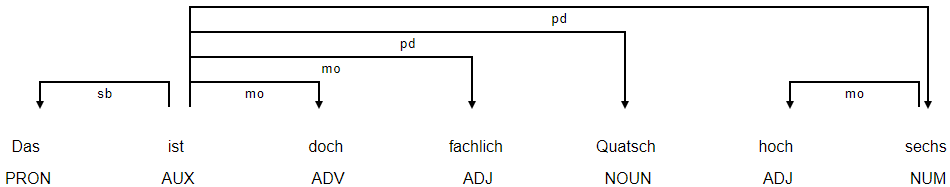
\includegraphics[width=1\textwidth]{chapters/04-Sentiment-Analyse/steffi.png}}
\caption{Visualisierung der Wortabhängigkeiten (Zitat von Steffi Lemke MdB, 208. Sitzung, 10.02.2021)}
\label{steffi}
\end{figure}

\subsection{Negations-Erkennung}
\label{neg-erkennung}
Negation, also Ablehnung, Verneinung oder Aufhebung, hat einen erheblichen Einfluss auf das Ergebnis und damit die Korrektheit der Sentimentanalyse, weshalb in dieser Arbeit ein besonderes Augenmerk auf ihre Erkennung gelegt wurde. 
In \textit{Negation Modeling for German Polarity Classification} \cite{g3_wieg} präsentieren Forscher der Universität des Saarlandes und des Leibniz-Institut für Deutsche Sprache hierfür einen regelbasierten Ansatz. 

Sie definieren unterschiedliche Negationstypen und ihre jeweilige Reichweite. 
So beeinflussen etwa negierende Adverbien oder Indefinitpronomen wie \textit{nie} den gesamten Satz, wohingegen das Partikel \textit{nicht} lediglich seinen Vorgänger negiert.  
Die Tabelle \ref{g3tab1} führt alle in dieser Arbeit implementierten Negationsregeln auf. 
Die Nutzung eines Abhängigkeitsbaumes, wie von \mintinline{latex}{spaCy} ermittelt, ist dabei unerlässlich. 
Denn wie schon im vorherigen Kapitel angesprochen, ist etwa mit dem Vorgänger eines Wortes nicht das in der Satzabfolge voranstehende Wort gemeint, sondern vielmehr der semantische Regent. 

\begin{table}[htbp]
\caption{Implementierte Negations-Regeln aus \cite{g3_wieg}}
\begin{center}
\begin{tabular}{| c | c | c |}
\hline
\textbf{Negationstyp} & \textbf{Reichweite} & \textbf{Beispielworte} \\ \hline
Partikel & Vorgänger (Regent) & nicht \\ \hline
Präpositionen & Nachfolger (Dependent) & ohne, gegen \\ \hline
Adverbien, & Satz & nie, kein, kaum \\
Indefinitpronomen &  &  \\ \hline
Nomen & Genitiv,& Abschaffung, \\
 & Präpositionalobjekt & Zerstörung \\ \hline
Verben & Objekt, Subjekt & enden, sinken, lindern \\
\hline
\end{tabular}
\label{g3tab1}
\end{center}
\end{table}

Angemerkt sei an dieser Stelle, dass es nicht möglich war, alle Regeln aus \cite{g3_wieg} zu implementieren, da der von den Forschern genutzte Dependency-Parser umfangreichere Ergebnisse liefert, als jener von \mintinline{latex}{spaCy}. 

Eine Liste mit Negationsworten und dem jeweiligen Negationstyp wurde \cite{g3_polcla} entnommen und ist ebenfalls über die Klasse \mintinline{latex}{Lexicon} zugreifbar. 
Die Klasse stellt ein \mintinline{latex}{Dictionary} bereit, in welchem die Schlüssel die Negationsworte und die Werte eine Liste der Reichweiten sind. 

Wenn in einem Text ein Negationswort auftritt, werden alle implementierten Regeln geprüft. 
Sollte es zu einem Treffer kommen, etwa wenn das Wort \textit{nicht} auftritt (siehe Abb. \ref{brandner}) und es einen Vorgänger gibt, werden alle Worte in Reichweite des Negationswortes negiert. 
Dies geschieht, indem für die jeweiligen Worte, welche wie in \ref{g3textv} beschrieben \mintinline{latex}{Token}-Objekte sind, ein eigenes Attribut mit der Bezeichnung \mintinline{latex}{negated} auf \mintinline{latex}{True} gesetzt wird. 
In der Polaritätsberechnung wird wortweise auf dieses Attribut geprüft und die Wort-Polarität bei einer Negierung mit -1 multipliziert. 

\begin{figure}[htb]
\centerline{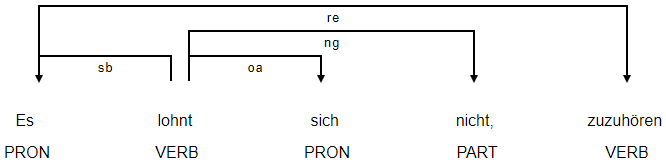
\includegraphics[width=1\textwidth]{chapters/04-Sentiment-Analyse/brandner.png}}
\caption{Beispielsatz mit Patikel-Negation (Zitat von Stephan Brandner MdB, 207. Sitzung, 29.01.2021)}
\label{brandner}
\end{figure}

\subsection{Verstärkungs-Erkennung}
\label{ver-erkennung}
Als \textit{Verstärker} werden sog. Gradpartikel (z.B. sehr, besonders, viel) verstanden, welche direkt vor Adjektiven oder Adverbien in einem Satz auftreten. 
Sie verstärken ihren Nachfolger, was wiederum in der Polaritätsberechnung berücksichtigt werden soll. 

Aus diesem Grund wird eine Liste mit verstärkenden Gradpartikeln, welche ebenfalls aus \cite{g3_polcla} bezogen werden, eingelesen und über die \mintinline{latex}{Lexicon} Klasse bereitgestellt. 

Ebenso wie in Kapitel \ref{neg-erkennung} bereits für die Negation beschrieben, wird ein eigenes Attribut zur Signalisierung einer Verstärkung definiert und im entsprechenden Fall auf True gesetzt. 
Bei der Polaritätsberechnung wird bei einer erkannten Verstärkung die Wort-Polarität mit 1,5 multipliziert \cite{g3_sentia}. 

In Abbildung \ref{hessel} wird ein Beispiel für das Auftreten eines verstärkenden Gradpartikels gegeben. 
Hier verstärkt das Wort \textit{sehr} das negative Wort \textit{spät}, womit die errechnete Polarität stärker negativ ausfällt als ohne die Verstärkungs-Erkennung. 

\begin{figure}[htb]
\centerline{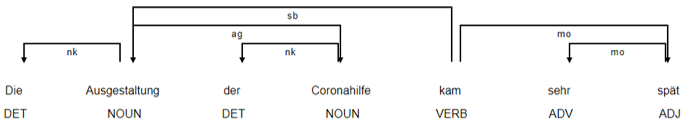
\includegraphics[width=1\textwidth]{chapters/04-Sentiment-Analyse/hessel.png}}
\caption{Beispielsatz mit Gradpartikel-Verstärkung (Zitat von Katja Hessel MdB, 206. Sitzung, 28.01.2021)}
\label{hessel}
\end{figure}

\subsection{Polaritätsberechnung}
\label{polberechnung}
Für die abschließende Berechnung der Polarität sind verschiedene Formeln denkbar. 
Sie sollten anhand von Textcharakteristika wie z.B. der Satz- oder Textlänge gewählt werden. 

Bei der Verwendung einer satzbasierten Polaritätsberechnung, bei welcher alle Polaritäten erst addiert und die Summe anschließend durch die Anzahl der Worte dividiert wird, kann ein unerwünschtes Phänomen auftreten: 
Längere Sätze erhaltenen ein stärker polarisiertes Ergebnis als vergleichbare kurze Sätze. 

Dies ist mit einer im Schnitt höheren Dichte an Worten mit Polaritäts-Wert in längeren Sätzen zu erklären. 
Um diesem Problem entgegen zu wirken, wurde in dieser Arbeit eine Min-Max-Skalierung (siehe Formeln 1 - 3) auf Dokumentebene implementiert \cite{g3_sentia}. 

Die Entscheidung, diese Normalisierung anhand der Länge des gesamten Textes durchzuführen, wurde aufgrund der Charakteristika der zu analysierenden Interaktionen getroffen. 
Denn diese bestehen zu einem überwiegenden Teil aus einem einzelnen Satz von jedoch sehr unterschiedlicher Länge. 

\begin{align}
p' &= \frac{ p + 1 }{ text.len + 1 } \text{ für p $>$ 0}\\
p' &= \frac{ p - 1 }{ text.len + 1 } \text{ für p $<$ 0}\\
p' &= p \text{ für p $=$ 0}
\end{align}

\section{Evaluierung}
\subsection{Sprache im Bundestag}
\label{sprachebundestag}
Während der Entwicklung dieser Arbeit und den regelmäßig angestellten Zwischentests wurde ersichtlich, dass sich die Sprache im Bundestag etwa von jener in sozialen Netzwerken oder Produktbewertungen unterschiedet. 
Ein Interaktionstext setzt sich sowohl aus einzelnen, langen und komplexe Sätze zusammen, als auch aus einzelnen Ausrufen wie \textit{\glqq eieiei!\grqq} zusammen. 

Aus diesem Grund wurde die in \ref{polberechnung} beschriebene Normalisierung verwendet, da herkömmliche Berechnungsformeln zunächst widersprüchliche Ergebnisse lieferten. 
Gleichzeitig verbesserte die manuelle Durchsicht der häufigsten 15.000 Worte und Anfertigung einer eigenen Bundestags-Wortliste das Ergebnis deutlich. 
Viele der regelmäßig in Bundestagssitzungen verwendeten Worte gehören zur \textit{Politik-Domäne} und treten deshalb nicht in den Quell-Wortlisten auf. 
Hier wird erwartet, dass eine noch umfangreichere Bundestags-Wortliste einen weiteren positiven Einfluss auf das Endergebnis hätte. 
Aus Zeit- sowie Kompetenzgründen wurde diese Liste jedoch nicht erweitert. 

\subsection{Ironie und Sarkasmus}
Ebenso wie die im vorherigen besprochene \textit{Politiksprache}, treten auch Ironie und Sarkasmus vermehrt in den Sitzungen des Bundestages auf. 
Einfach umrissen, handelt es sich dabei um ein Stilmittel, bei dem das Gegenteil vom Gesagten gemeint ist. 
Sarkasmus ist dabei eine verstärkte Form der Ironie und kann auch als ein Angriff verstanden werden. 

Selbst für den menschlichen Leser ist allein am geschriebenen Text nicht immer ersichtlich, ob eine Aussage ironisch gemeint ist. 
Vielmehr wird für die richtige Deutung die Stimmlage, Gestik und Mimik der sprechenden Person benötigt. 

Ironie und Sarkasmus könne also erst recht nicht mit dem in dieser Arbeit verwendeten Wortlisten-Ansatz erkannt werden, womit ein unbekannter Teil der Interaktionen im Ergebnis die falsche Polarität besitzt. 
Gleichwohl gibt es Ansätze aus dem Bereich des maschinellen Lernens, welche dieses Problem behandeln. 
Jedoch setzen diese einen entsprechend annotierten Korpus vorraus und stammen zudem aus dem Bereich der sozialen Netzwerke, in welchen etwa mit \textit{Hashtags} die Ironie bereits vom Autor markiert wurde. 

\subsection{Fazit}
Trotzt der soeben beschriebenen Fehlerquellen, wurde dennoch ein gelungenes Ergebnis erzielt: 
Es wurde ein solider und erweiterbarer Algorithmus zur Sentimentananlyse von Texten geschaffen, welcher auf den bekanntesten Bibliotheken und Techniken der Textverarbeitung beruht. 
Dieser kann als Basis für weitere Anstrengungen bei der Sentimentanalyse von politischen Texten dienen. 

Eine Deutung der bisherigen Ergebnisse durch Politikwissenschaftler oder anderweitig in diesem Bereich kompetente Personen wird dabei empfohlen, um die beschriebenen Schwachstellen entsprechend zu behandeln oder neue zu identifizieren. 

Der Programmcode ist zudem vollständig und abgesichert in die Projektpipeline eingebunden. 
Er erweitert seine Ergebnis-Datenbank automatisch um neue Sitzungen und benachrichtigt anschließend nachfolgende Gruppen. 

\section{Grundlagen}\label{sec:07_02_grundlagen}
\section{Anforderungsanalyse und Konzept}\label{sec:08_03_anforderungen_konzept}


\section{Zusammenfassung und Ausblick}\label{sec:07_05_zusammenfassung}

\chapter{Graphauswertung}
\section{Einleitung}
Der Begriff \textit{Sentiment} stammt vom lateinischen Wort \textit{sentimentum} ab und bedeutet Empfindung oder Stimmung. 
In der Sentimentanalyse geht es um die Bestimmung eben jener Stimmung einer Meinungsäußerung. 
Anwendung findet sie etwa bei Produktbewertungen oder Beiträgen in sozialen Netzwerken. 
Die Stimmung wird durch die sog. Polarität beschrieben und kann positiv, negativ oder neutral ausfallen. 
Im Text-Mining wird sie im Intervall $\interval{-1}{1} = \{x \in \mathbb{R} | -1 \leq x \leq 1\}$ angegeben, wobei -1 sehr negativ, 1 sehr positiv und 0 neutral bedeuten. 

Grundlegend ist die maschinelle Sentimentanalyse entweder Wortlisten- oder Modell-basiert. 
Der Wortlisten-Ansatz kann als eine Sammlung von Worten und ihrer Polaritäten verstanden werden, anhand welcher die Stimmung berechnet wird. 
Dieser Ansatz wird weiter im Kapitel \ref{wortliste} beschrieben, da er in dieser Arbeit verwendet wurde. 

Bei der Modell-basierten Sentimentanalyse wird ein annotierter Satz-Korpus für das Trainieren einer künstlichen Intelligenz vorausgesetzt. 
Etwa für Twitter-Beiträge stehen solche Korpusse oder auch bereits trainierte Modelle zur Verfügung. 
Jedoch ist bei der Verwendung zur Analyse der Sitzungsprotokolle des Bundestages nicht mit zufriedenstellenden Ergebnissen zu rechnen, da sich verwendete Worte und Text- bzw. Satzbau zwischen diesen Domänen deutlich unterscheiden. 
Eine weitere Erläuterung zur Sprache im Bundestag wird in Kapitel \ref{sprachebundestag} gegeben. 

Ebenfalls werden die Komponenten zur Teilnahme an der Verarbeitungspipeline des Gesamtprojektes im nachfolgenden Kapitel \ref{g3daten} beschrieben. 

\section{Datenaustausch}
\label{g3daten}
\subsection{Datenimport}
Für das Erhalten von Daten wurde eine Methode implementiert, welche durch Angabe einer Sitzungs-ID die entsprechende Sitzung vom REST-API von Gruppe 2 abfragen kann. 
Diese Methode gibt jede Sitzung weiter an die in Kapitel \ref{g3textv} beschriebene Textverarbeitung und das Ergebnis schließlich an den in Kapitel \ref{g3export} beschriebenen Export-Code. 

Die Methode wird für zwei Fälle verwendet: 
Beim Normalfall sendet die Gruppe 2 eine Benachrichtigung mit einer Liste aller neuen Sitzungs-IDs an das REST-API im Code dieser Arbeit. 
Das REST-API wurde mit der Bibliothek \mintinline{latex}{Flask} \cite{g3_flask} entwickelt und besteht aus einer POST-Schnittstelle, welche auf dem von der HTW bereitgestelltem Server unter \textit{/notify} erreichbar ist. 

Das API wurde unter Zuhilfenahme von \mintinline{latex}{Flask.Blueprints} \cite{g3_flaskbp} entwickelt und wird von einem \mintinline{latex}{Waitress}-Webserver \cite{g3_waitress} bereitgestellt. 
Für jede Anfrage wird geprüft, ob Content-Type und Payload dem erwarteten JSON-Daten entsprechen. 
Sollte dies nicht der Fall sein, wird eine entsprechende Rückmeldung an den Sender zurückgegeben. 
Für jede erhaltene Sitzungs-ID wird die eingangs beschriebene Methode aufgerufen. 

Der zweite Fall wurde vor allem im Rahmen der voranschreitenden Entwicklung bei den in der Projektpipeline voranstehenden Gruppen verwendet. 
Statt auf eine Benachrichtigung zum Anstoßen des Datenimports zu warten, werden stattdessen alle Sitzungs-IDs vom REST-API der Gruppe 2 abgefragt und jede Sitzung vollständig neu importiert. 
Dieses Vorgehen hat den Vorteil, dass eventuell durch Arbeit am Code verpasste Benachrichtigungen nachgeholt werden und gleichzeitig Änderungen an den Daten übernommen werden können. 

\subsection{Datenexport}
\label{g3export}
Statt Arbeit in ein umfangreiches REST-API für die nachfolgenden Gruppen zu stecken, wurde für diese Arbeit ein reiner MongoDB-Ansatz verwendet. 
Auf dem zur Verfügung stehenden HTW-Server wurde dafür eine MongoDB Instanz aufgesetzt, welche nur aus dem HTW-Netz erreichbar und zudem nur mit Authentifizierung zugreifbar ist. 
Jede Sitzung ist hier als eine eigene Collection persistiert. 
Sobald neue Sitzungen importiert und verarbeitet wurden, werden diese zunächst mit dem MongoDB-Treiber \mintinline{latex}{PyMongo} \cite{g3_mongodb} in die Datenbank geschrieben. 
Anschließend werden die nachfolgenden Gruppen mit einem POST and die jeweilige REST-Schnittstelle benachrichtigt, dass neue Daten vorliegen. 
Diese greifen dann mit den zuvor versendeten Zugangsdaten direkt auf die Datenbank zu. 

Mit diesem Vorgehen konnte die Komplexität beim Zugriff auf die Ergebnis-Daten gesenkt werden, da es für nahezu alle gängigen Programmiersprachen einen intuitiven MongoDB-Treiber gibt. 

\section{Wortliste}
\label{wortliste}
Wie bereits in der Einleitung beschrieben, handelt es sich bei Wortlisten in der Sentimentanalyse um eine Liste von Worten und ihrer jeweiligen Polarität. 
Bei der Analyse eines Textes wird wortweise ein Abgleich mit dieser Liste durchgeführt und die Wort-Polarität bei einer Übereinstimmung für die Berechnung des Sentiments verwendet. 
Unterschiedliche Berechnungsformeln sind dabei denkbar und werden in Kapitel \ref{polberechnung} weiter besprochen. 
Für diese Arbeit wurden Wortlisten verschiedener Institutionen kombiniert und anschließend mit Synonymen erweitert. 
Ebenfalls wurde eine eigene Bundestags-Wortliste erstellt. 

Die Interest Group on German Sentiment Analysis (IGGSA) stellt eine umfangreiche Liste an Publikationen und Ressourcen zu Sentimentanalysen in der deutschen Sprache zur Verfügung \cite{g3_iggsa}. 
Hier wurden alle Referenzen auf die in dieser Arbeit verwendeten Quell-Wortlisten gesammelt. 
Für die Zusammenführung dieser Wortlisten wurden zunächst zwei Herangehensweisen evaluiert: 
Zum einen war die Erstellung eines eigenständigen Codes denkbar, welcher einmalig die Daten aus allen Quellen einliest, zusammenfasst und eine Ergebnis-Datei ausgibt. 
Diese Datei wäre eine Ressource für den eigentlichen Analyse-Code. 
Zum anderen könnte die soeben beschriebene Funktionalität jedoch auch direkt im Analyse-Code integriert und bei jedem Programmstart ausgeführt werden. 
Die kombinierte Wortliste würde somit nicht auf die Festplatte geschrieben, sondern im Arbeitsspeicher verbleiben, solange der Analyse-Code läuft. 
Wenngleich der zuerst beschriebene Ansatz offensichtlich weniger Rechenzeitaufwändig ist, wurde für diese Arbeit der zweite Ansatz gewählt. 
Dies wird vor allem mit Rechtsunsicherheiten bei der Arbeit mit den verschiedenen Lizenzen der Quelldateien begründet. 
Gleichzeitig arbeitet der Analyse-Code damit jederzeit mit dem aktuellen Stand der Quell-Wortlisten. 
Das Aufbauen der Wortliste dauert wenige Minuten. 

Für diese Arbeit wurden die folgenden Quell-Wortlisten verwendet: 

\begin{itemize}
\item \textit{SentimentWortschatz} (SentiWS) aus \glqq SentiWS - a Publicly Available German-language Resource for Sentiment Analysis\grqq (Universität Leipzig) \cite{g3_sentiws}
\item \textit{Multi-Domain Sentiment Lexicon for German} (Hochschule Darmstadt) \cite{g3_opm}
\item \textit{German Polarity Lexicon} aus \glqq Evaluation and extension of a polarity lexicon for German\grqq (Universität Zürich) \cite{g3_polcla}
\item \textit{morphcomp} aus \glqq Evaluating the morphological compositionality of pola-rity\grqq (Leibniz-Institut für Deutsche Sprache, Universität des Saarlandes) \cite{g3_morphcomp}
\end{itemize}

Aus diesen Quellen ergibt sich eine Wortliste mit etwa 14.000 einzigartigen Worten. 
Die Worte werden dabei mit der in Kapitel \ref{g3textv} beschriebenen Textverarbeitungspipeline lemmatisiert, also auf die Grundform zurückgeführt. 
Bei Überschneidungen wird ein Mittelwert über alle Polaritäts-Werte eines Wortes gebildet. 

Mithilfe des \textit{Open German WordNet} (OdeNet) \cite{g3_odenet} werden zu jedem Wort Synonyme gesammelt und ebenfalls der Wortliste hinzugefügt. 
Der Zugriff auf OdeNet geschieht dabei mit der python Bibliothek \mintinline{latex}{WN} \cite{g3_wn}. 
Die Verwendung dieser Bibliothek ist trivial, weshalb an dieser Stelle keine weitere Erläuterung gegeben wird. 
Die Wortliste wird durch das Hinzufügen von Synonymen um weitere rund 2.000 Worte erweitert. 

Wie bereits in der Einleitung erwähnt, wurde zudem eine eigene Bundes-tags-Wortliste erstellt. 
Hierzu wurden die 15.000 am häufigsten in den Sitzungsprotokollen vorkommenden Worte erfasst und analysiert. 
Dabei wurden jedoch nur jene Worte betrachtet, welche nicht bereits in der kombinierten Wortliste vorkommen. 
Ausgewählt wurden nur eindeutig positive oder negative Worte wie \textit{angemessen}, \textit{Bullshit}, \textit{Fehlentscheidung}, \textit{Milchmädchenrechnung}, \textit{Realitätsverweigerung}, \textit{Totalausfall} oder \textit{Verunglimpfung}. 
Insgesamt umfasst die Bundestags-Wortliste 217 Worte. 

Im Code wird der Zugriff auf die Wortliste mit der zentralen Klasse \mintinline{latex}{Lexicon} realisiert. 
Bei der Instanziierung der Klasse werden, wie im Vorherigen beschrieben, alle Wortlisten gesammelt, zusammengeführt und erweitert. 
Anschließend stellt die Klasse ein \mintinline{latex}{Dictionary} bereit, in welchem die Schlüssel die Worte und die Werte die Wort-Polarität angeben. 

\section{Textverarbeitung}
\label{g3textv}
Für die Textverarbeitung nutzt der Code dieser Arbeit vollständig die Funktionalitäten und Strukturen von \mintinline{latex}{spaCy} \cite{g3_spacy}. 
Die \mintinline{latex}{spaCy} Bibliothek stellt eine Textverarbeitungspipeline bereit, welche mithilfe eines vortrainierten Modells funktioniert. 
Für die deutsche Sprache wurde ein solches Modell mit dem TIGER Korpus der Universität Stuttgart trainiert. 
Der Korpus umfasst ca. 50.000 Sätze aus Texten der Frankfurter Rundschau. 
Die \mintinline{latex}{spaCy}-Pipeline besteht aus den folgenden Komponenten: 

\begin{itemize}
\item Tokenisierung (Text- und Satzzerteilung)
\item POS-Tagging (Wortartenerkennung)
\item Dependency-Parsing (Wortabhängigkeitenerkennung)
\item Lemmatisierung (Wortgrundformermittlung)
\item Entity-Recognition (Eigennamenerkennung)
\end{itemize}

Das Ergebnis der Pipeline ist ein \mintinline{latex}{Doc}-Objekt, welches das Ergebnis des gesamten in die Pipeline gegebenen Textes umfasst. 
Einzelne Sätze innerhalb des \mintinline{latex}{Doc}-Objektes werden mit \mintinline{latex}{Span}-Objekten beschrieben und einzelne Worte mit \mintinline{latex}{Token}-Objekten. 
Die Objekttypen besitzen jeweils eigene Methoden und Erweiterungsmöglichkeiten in Form von sog. \textit{extension attributes}. 

Sehr einfach und gleichzeitig umfangreich kann die \mintinline{latex}{spaCy}-Pipeline an die eigenen Bedürfnisse angepasst werden. 
So wurde die Berechnung des Sentiments eines Textes direkt an die Komponenten der Standart-Pipeline angehängt. 
Logisch unterteilt sich diese in die Komponenten:

\begin{itemize}
\item Negations-Erkennung (siehe \ref{neg-erkennung})
\item Verstärkungs-Erkennung (siehe \ref{ver-erkennung})
\item Polaritätsberechnung (siehe \ref{polberechnung})
\end{itemize}

Basis für das nachfolgende Kapitel \ref{neg-erkennung} ist dabei das Ergebnis des Depen-dency-Parsers von \mintinline{latex}{spaCy}. 
Dieser bestimmt die Abhängigkeiten zwischen den einzelnen Elementen eines Satzes. 
Diese Funktion gehört dem Themenbereich der Dependenzgrammatik an, in welcher gerichtete Beziehungen zwischen den Worten eines Satzes beschreibt werden. 
Ein Wort kann einen Vorgänger (Regent) und mehrere Nachfolger (Dependenten) besitzen. 
Die Gesamtheit der Beziehungen eines Satzes wird auch Abhängigkeitsbaum genannt. 

Zur Verdeutlichung soll die Abbildung \ref{steffi} dienen, welche mithilfe von \mintinline{latex}{spaCy.displaCy} erstellt wurde. 
Zu sehen ist hier der Abhängigkeitsbaum des Satzes \textit{\glqq Das ist doch fachlich Quatsch hoch sechs!\grqq}. 
An den gerichteten Kanten befindet sich die Angabe des Satzgliedes, unterhalb der Worte die Angabe der Wortart. 

\begin{figure}[htb]
\centerline{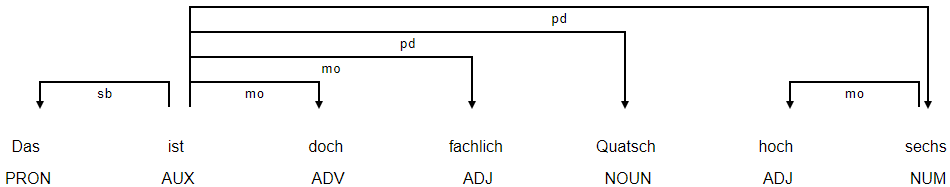
\includegraphics[width=1\textwidth]{chapters/04-Sentiment-Analyse/steffi.png}}
\caption{Visualisierung der Wortabhängigkeiten (Zitat von Steffi Lemke MdB, 208. Sitzung, 10.02.2021)}
\label{steffi}
\end{figure}

\subsection{Negations-Erkennung}
\label{neg-erkennung}
Negation, also Ablehnung, Verneinung oder Aufhebung, hat einen erheblichen Einfluss auf das Ergebnis und damit die Korrektheit der Sentimentanalyse, weshalb in dieser Arbeit ein besonderes Augenmerk auf ihre Erkennung gelegt wurde. 
In \textit{Negation Modeling for German Polarity Classification} \cite{g3_wieg} präsentieren Forscher der Universität des Saarlandes und des Leibniz-Institut für Deutsche Sprache hierfür einen regelbasierten Ansatz. 

Sie definieren unterschiedliche Negationstypen und ihre jeweilige Reichweite. 
So beeinflussen etwa negierende Adverbien oder Indefinitpronomen wie \textit{nie} den gesamten Satz, wohingegen das Partikel \textit{nicht} lediglich seinen Vorgänger negiert.  
Die Tabelle \ref{g3tab1} führt alle in dieser Arbeit implementierten Negationsregeln auf. 
Die Nutzung eines Abhängigkeitsbaumes, wie von \mintinline{latex}{spaCy} ermittelt, ist dabei unerlässlich. 
Denn wie schon im vorherigen Kapitel angesprochen, ist etwa mit dem Vorgänger eines Wortes nicht das in der Satzabfolge voranstehende Wort gemeint, sondern vielmehr der semantische Regent. 

\begin{table}[htbp]
\caption{Implementierte Negations-Regeln aus \cite{g3_wieg}}
\begin{center}
\begin{tabular}{| c | c | c |}
\hline
\textbf{Negationstyp} & \textbf{Reichweite} & \textbf{Beispielworte} \\ \hline
Partikel & Vorgänger (Regent) & nicht \\ \hline
Präpositionen & Nachfolger (Dependent) & ohne, gegen \\ \hline
Adverbien, & Satz & nie, kein, kaum \\
Indefinitpronomen &  &  \\ \hline
Nomen & Genitiv,& Abschaffung, \\
 & Präpositionalobjekt & Zerstörung \\ \hline
Verben & Objekt, Subjekt & enden, sinken, lindern \\
\hline
\end{tabular}
\label{g3tab1}
\end{center}
\end{table}

Angemerkt sei an dieser Stelle, dass es nicht möglich war, alle Regeln aus \cite{g3_wieg} zu implementieren, da der von den Forschern genutzte Dependency-Parser umfangreichere Ergebnisse liefert, als jener von \mintinline{latex}{spaCy}. 

Eine Liste mit Negationsworten und dem jeweiligen Negationstyp wurde \cite{g3_polcla} entnommen und ist ebenfalls über die Klasse \mintinline{latex}{Lexicon} zugreifbar. 
Die Klasse stellt ein \mintinline{latex}{Dictionary} bereit, in welchem die Schlüssel die Negationsworte und die Werte eine Liste der Reichweiten sind. 

Wenn in einem Text ein Negationswort auftritt, werden alle implementierten Regeln geprüft. 
Sollte es zu einem Treffer kommen, etwa wenn das Wort \textit{nicht} auftritt (siehe Abb. \ref{brandner}) und es einen Vorgänger gibt, werden alle Worte in Reichweite des Negationswortes negiert. 
Dies geschieht, indem für die jeweiligen Worte, welche wie in \ref{g3textv} beschrieben \mintinline{latex}{Token}-Objekte sind, ein eigenes Attribut mit der Bezeichnung \mintinline{latex}{negated} auf \mintinline{latex}{True} gesetzt wird. 
In der Polaritätsberechnung wird wortweise auf dieses Attribut geprüft und die Wort-Polarität bei einer Negierung mit -1 multipliziert. 

\begin{figure}[htb]
\centerline{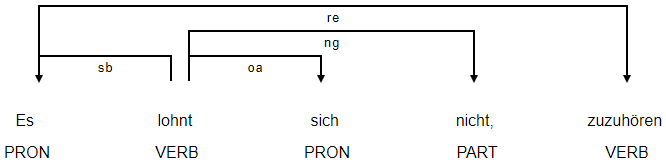
\includegraphics[width=1\textwidth]{chapters/04-Sentiment-Analyse/brandner.png}}
\caption{Beispielsatz mit Patikel-Negation (Zitat von Stephan Brandner MdB, 207. Sitzung, 29.01.2021)}
\label{brandner}
\end{figure}

\subsection{Verstärkungs-Erkennung}
\label{ver-erkennung}
Als \textit{Verstärker} werden sog. Gradpartikel (z.B. sehr, besonders, viel) verstanden, welche direkt vor Adjektiven oder Adverbien in einem Satz auftreten. 
Sie verstärken ihren Nachfolger, was wiederum in der Polaritätsberechnung berücksichtigt werden soll. 

Aus diesem Grund wird eine Liste mit verstärkenden Gradpartikeln, welche ebenfalls aus \cite{g3_polcla} bezogen werden, eingelesen und über die \mintinline{latex}{Lexicon} Klasse bereitgestellt. 

Ebenso wie in Kapitel \ref{neg-erkennung} bereits für die Negation beschrieben, wird ein eigenes Attribut zur Signalisierung einer Verstärkung definiert und im entsprechenden Fall auf True gesetzt. 
Bei der Polaritätsberechnung wird bei einer erkannten Verstärkung die Wort-Polarität mit 1,5 multipliziert \cite{g3_sentia}. 

In Abbildung \ref{hessel} wird ein Beispiel für das Auftreten eines verstärkenden Gradpartikels gegeben. 
Hier verstärkt das Wort \textit{sehr} das negative Wort \textit{spät}, womit die errechnete Polarität stärker negativ ausfällt als ohne die Verstärkungs-Erkennung. 

\begin{figure}[htb]
\centerline{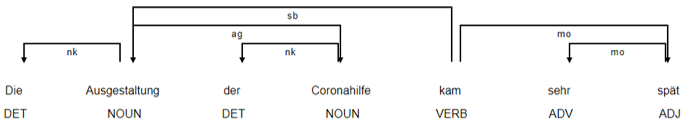
\includegraphics[width=1\textwidth]{chapters/04-Sentiment-Analyse/hessel.png}}
\caption{Beispielsatz mit Gradpartikel-Verstärkung (Zitat von Katja Hessel MdB, 206. Sitzung, 28.01.2021)}
\label{hessel}
\end{figure}

\subsection{Polaritätsberechnung}
\label{polberechnung}
Für die abschließende Berechnung der Polarität sind verschiedene Formeln denkbar. 
Sie sollten anhand von Textcharakteristika wie z.B. der Satz- oder Textlänge gewählt werden. 

Bei der Verwendung einer satzbasierten Polaritätsberechnung, bei welcher alle Polaritäten erst addiert und die Summe anschließend durch die Anzahl der Worte dividiert wird, kann ein unerwünschtes Phänomen auftreten: 
Längere Sätze erhaltenen ein stärker polarisiertes Ergebnis als vergleichbare kurze Sätze. 

Dies ist mit einer im Schnitt höheren Dichte an Worten mit Polaritäts-Wert in längeren Sätzen zu erklären. 
Um diesem Problem entgegen zu wirken, wurde in dieser Arbeit eine Min-Max-Skalierung (siehe Formeln 1 - 3) auf Dokumentebene implementiert \cite{g3_sentia}. 

Die Entscheidung, diese Normalisierung anhand der Länge des gesamten Textes durchzuführen, wurde aufgrund der Charakteristika der zu analysierenden Interaktionen getroffen. 
Denn diese bestehen zu einem überwiegenden Teil aus einem einzelnen Satz von jedoch sehr unterschiedlicher Länge. 

\begin{align}
p' &= \frac{ p + 1 }{ text.len + 1 } \text{ für p $>$ 0}\\
p' &= \frac{ p - 1 }{ text.len + 1 } \text{ für p $<$ 0}\\
p' &= p \text{ für p $=$ 0}
\end{align}

\section{Evaluierung}
\subsection{Sprache im Bundestag}
\label{sprachebundestag}
Während der Entwicklung dieser Arbeit und den regelmäßig angestellten Zwischentests wurde ersichtlich, dass sich die Sprache im Bundestag etwa von jener in sozialen Netzwerken oder Produktbewertungen unterschiedet. 
Ein Interaktionstext setzt sich sowohl aus einzelnen, langen und komplexe Sätze zusammen, als auch aus einzelnen Ausrufen wie \textit{\glqq eieiei!\grqq} zusammen. 

Aus diesem Grund wurde die in \ref{polberechnung} beschriebene Normalisierung verwendet, da herkömmliche Berechnungsformeln zunächst widersprüchliche Ergebnisse lieferten. 
Gleichzeitig verbesserte die manuelle Durchsicht der häufigsten 15.000 Worte und Anfertigung einer eigenen Bundestags-Wortliste das Ergebnis deutlich. 
Viele der regelmäßig in Bundestagssitzungen verwendeten Worte gehören zur \textit{Politik-Domäne} und treten deshalb nicht in den Quell-Wortlisten auf. 
Hier wird erwartet, dass eine noch umfangreichere Bundestags-Wortliste einen weiteren positiven Einfluss auf das Endergebnis hätte. 
Aus Zeit- sowie Kompetenzgründen wurde diese Liste jedoch nicht erweitert. 

\subsection{Ironie und Sarkasmus}
Ebenso wie die im vorherigen besprochene \textit{Politiksprache}, treten auch Ironie und Sarkasmus vermehrt in den Sitzungen des Bundestages auf. 
Einfach umrissen, handelt es sich dabei um ein Stilmittel, bei dem das Gegenteil vom Gesagten gemeint ist. 
Sarkasmus ist dabei eine verstärkte Form der Ironie und kann auch als ein Angriff verstanden werden. 

Selbst für den menschlichen Leser ist allein am geschriebenen Text nicht immer ersichtlich, ob eine Aussage ironisch gemeint ist. 
Vielmehr wird für die richtige Deutung die Stimmlage, Gestik und Mimik der sprechenden Person benötigt. 

Ironie und Sarkasmus könne also erst recht nicht mit dem in dieser Arbeit verwendeten Wortlisten-Ansatz erkannt werden, womit ein unbekannter Teil der Interaktionen im Ergebnis die falsche Polarität besitzt. 
Gleichwohl gibt es Ansätze aus dem Bereich des maschinellen Lernens, welche dieses Problem behandeln. 
Jedoch setzen diese einen entsprechend annotierten Korpus vorraus und stammen zudem aus dem Bereich der sozialen Netzwerke, in welchen etwa mit \textit{Hashtags} die Ironie bereits vom Autor markiert wurde. 

\subsection{Fazit}
Trotzt der soeben beschriebenen Fehlerquellen, wurde dennoch ein gelungenes Ergebnis erzielt: 
Es wurde ein solider und erweiterbarer Algorithmus zur Sentimentananlyse von Texten geschaffen, welcher auf den bekanntesten Bibliotheken und Techniken der Textverarbeitung beruht. 
Dieser kann als Basis für weitere Anstrengungen bei der Sentimentanalyse von politischen Texten dienen. 

Eine Deutung der bisherigen Ergebnisse durch Politikwissenschaftler oder anderweitig in diesem Bereich kompetente Personen wird dabei empfohlen, um die beschriebenen Schwachstellen entsprechend zu behandeln oder neue zu identifizieren. 

Der Programmcode ist zudem vollständig und abgesichert in die Projektpipeline eingebunden. 
Er erweitert seine Ergebnis-Datenbank automatisch um neue Sitzungen und benachrichtigt anschließend nachfolgende Gruppen. 

\section{Grundlagen}\label{sec:07_02_grundlagen}
\section{Anforderungsanalyse und Konzept}\label{sec:08_03_anforderungen_konzept}


\section{Zusammenfassung und Ausblick}\label{sec:07_05_zusammenfassung}

\chapter{Benutzeroberfläche}
\section{Einleitung}
Der Begriff \textit{Sentiment} stammt vom lateinischen Wort \textit{sentimentum} ab und bedeutet Empfindung oder Stimmung. 
In der Sentimentanalyse geht es um die Bestimmung eben jener Stimmung einer Meinungsäußerung. 
Anwendung findet sie etwa bei Produktbewertungen oder Beiträgen in sozialen Netzwerken. 
Die Stimmung wird durch die sog. Polarität beschrieben und kann positiv, negativ oder neutral ausfallen. 
Im Text-Mining wird sie im Intervall $\interval{-1}{1} = \{x \in \mathbb{R} | -1 \leq x \leq 1\}$ angegeben, wobei -1 sehr negativ, 1 sehr positiv und 0 neutral bedeuten. 

Grundlegend ist die maschinelle Sentimentanalyse entweder Wortlisten- oder Modell-basiert. 
Der Wortlisten-Ansatz kann als eine Sammlung von Worten und ihrer Polaritäten verstanden werden, anhand welcher die Stimmung berechnet wird. 
Dieser Ansatz wird weiter im Kapitel \ref{wortliste} beschrieben, da er in dieser Arbeit verwendet wurde. 

Bei der Modell-basierten Sentimentanalyse wird ein annotierter Satz-Korpus für das Trainieren einer künstlichen Intelligenz vorausgesetzt. 
Etwa für Twitter-Beiträge stehen solche Korpusse oder auch bereits trainierte Modelle zur Verfügung. 
Jedoch ist bei der Verwendung zur Analyse der Sitzungsprotokolle des Bundestages nicht mit zufriedenstellenden Ergebnissen zu rechnen, da sich verwendete Worte und Text- bzw. Satzbau zwischen diesen Domänen deutlich unterscheiden. 
Eine weitere Erläuterung zur Sprache im Bundestag wird in Kapitel \ref{sprachebundestag} gegeben. 

Ebenfalls werden die Komponenten zur Teilnahme an der Verarbeitungspipeline des Gesamtprojektes im nachfolgenden Kapitel \ref{g3daten} beschrieben. 

\section{Datenaustausch}
\label{g3daten}
\subsection{Datenimport}
Für das Erhalten von Daten wurde eine Methode implementiert, welche durch Angabe einer Sitzungs-ID die entsprechende Sitzung vom REST-API von Gruppe 2 abfragen kann. 
Diese Methode gibt jede Sitzung weiter an die in Kapitel \ref{g3textv} beschriebene Textverarbeitung und das Ergebnis schließlich an den in Kapitel \ref{g3export} beschriebenen Export-Code. 

Die Methode wird für zwei Fälle verwendet: 
Beim Normalfall sendet die Gruppe 2 eine Benachrichtigung mit einer Liste aller neuen Sitzungs-IDs an das REST-API im Code dieser Arbeit. 
Das REST-API wurde mit der Bibliothek \mintinline{latex}{Flask} \cite{g3_flask} entwickelt und besteht aus einer POST-Schnittstelle, welche auf dem von der HTW bereitgestelltem Server unter \textit{/notify} erreichbar ist. 

Das API wurde unter Zuhilfenahme von \mintinline{latex}{Flask.Blueprints} \cite{g3_flaskbp} entwickelt und wird von einem \mintinline{latex}{Waitress}-Webserver \cite{g3_waitress} bereitgestellt. 
Für jede Anfrage wird geprüft, ob Content-Type und Payload dem erwarteten JSON-Daten entsprechen. 
Sollte dies nicht der Fall sein, wird eine entsprechende Rückmeldung an den Sender zurückgegeben. 
Für jede erhaltene Sitzungs-ID wird die eingangs beschriebene Methode aufgerufen. 

Der zweite Fall wurde vor allem im Rahmen der voranschreitenden Entwicklung bei den in der Projektpipeline voranstehenden Gruppen verwendet. 
Statt auf eine Benachrichtigung zum Anstoßen des Datenimports zu warten, werden stattdessen alle Sitzungs-IDs vom REST-API der Gruppe 2 abgefragt und jede Sitzung vollständig neu importiert. 
Dieses Vorgehen hat den Vorteil, dass eventuell durch Arbeit am Code verpasste Benachrichtigungen nachgeholt werden und gleichzeitig Änderungen an den Daten übernommen werden können. 

\subsection{Datenexport}
\label{g3export}
Statt Arbeit in ein umfangreiches REST-API für die nachfolgenden Gruppen zu stecken, wurde für diese Arbeit ein reiner MongoDB-Ansatz verwendet. 
Auf dem zur Verfügung stehenden HTW-Server wurde dafür eine MongoDB Instanz aufgesetzt, welche nur aus dem HTW-Netz erreichbar und zudem nur mit Authentifizierung zugreifbar ist. 
Jede Sitzung ist hier als eine eigene Collection persistiert. 
Sobald neue Sitzungen importiert und verarbeitet wurden, werden diese zunächst mit dem MongoDB-Treiber \mintinline{latex}{PyMongo} \cite{g3_mongodb} in die Datenbank geschrieben. 
Anschließend werden die nachfolgenden Gruppen mit einem POST and die jeweilige REST-Schnittstelle benachrichtigt, dass neue Daten vorliegen. 
Diese greifen dann mit den zuvor versendeten Zugangsdaten direkt auf die Datenbank zu. 

Mit diesem Vorgehen konnte die Komplexität beim Zugriff auf die Ergebnis-Daten gesenkt werden, da es für nahezu alle gängigen Programmiersprachen einen intuitiven MongoDB-Treiber gibt. 

\section{Wortliste}
\label{wortliste}
Wie bereits in der Einleitung beschrieben, handelt es sich bei Wortlisten in der Sentimentanalyse um eine Liste von Worten und ihrer jeweiligen Polarität. 
Bei der Analyse eines Textes wird wortweise ein Abgleich mit dieser Liste durchgeführt und die Wort-Polarität bei einer Übereinstimmung für die Berechnung des Sentiments verwendet. 
Unterschiedliche Berechnungsformeln sind dabei denkbar und werden in Kapitel \ref{polberechnung} weiter besprochen. 
Für diese Arbeit wurden Wortlisten verschiedener Institutionen kombiniert und anschließend mit Synonymen erweitert. 
Ebenfalls wurde eine eigene Bundestags-Wortliste erstellt. 

Die Interest Group on German Sentiment Analysis (IGGSA) stellt eine umfangreiche Liste an Publikationen und Ressourcen zu Sentimentanalysen in der deutschen Sprache zur Verfügung \cite{g3_iggsa}. 
Hier wurden alle Referenzen auf die in dieser Arbeit verwendeten Quell-Wortlisten gesammelt. 
Für die Zusammenführung dieser Wortlisten wurden zunächst zwei Herangehensweisen evaluiert: 
Zum einen war die Erstellung eines eigenständigen Codes denkbar, welcher einmalig die Daten aus allen Quellen einliest, zusammenfasst und eine Ergebnis-Datei ausgibt. 
Diese Datei wäre eine Ressource für den eigentlichen Analyse-Code. 
Zum anderen könnte die soeben beschriebene Funktionalität jedoch auch direkt im Analyse-Code integriert und bei jedem Programmstart ausgeführt werden. 
Die kombinierte Wortliste würde somit nicht auf die Festplatte geschrieben, sondern im Arbeitsspeicher verbleiben, solange der Analyse-Code läuft. 
Wenngleich der zuerst beschriebene Ansatz offensichtlich weniger Rechenzeitaufwändig ist, wurde für diese Arbeit der zweite Ansatz gewählt. 
Dies wird vor allem mit Rechtsunsicherheiten bei der Arbeit mit den verschiedenen Lizenzen der Quelldateien begründet. 
Gleichzeitig arbeitet der Analyse-Code damit jederzeit mit dem aktuellen Stand der Quell-Wortlisten. 
Das Aufbauen der Wortliste dauert wenige Minuten. 

Für diese Arbeit wurden die folgenden Quell-Wortlisten verwendet: 

\begin{itemize}
\item \textit{SentimentWortschatz} (SentiWS) aus \glqq SentiWS - a Publicly Available German-language Resource for Sentiment Analysis\grqq (Universität Leipzig) \cite{g3_sentiws}
\item \textit{Multi-Domain Sentiment Lexicon for German} (Hochschule Darmstadt) \cite{g3_opm}
\item \textit{German Polarity Lexicon} aus \glqq Evaluation and extension of a polarity lexicon for German\grqq (Universität Zürich) \cite{g3_polcla}
\item \textit{morphcomp} aus \glqq Evaluating the morphological compositionality of pola-rity\grqq (Leibniz-Institut für Deutsche Sprache, Universität des Saarlandes) \cite{g3_morphcomp}
\end{itemize}

Aus diesen Quellen ergibt sich eine Wortliste mit etwa 14.000 einzigartigen Worten. 
Die Worte werden dabei mit der in Kapitel \ref{g3textv} beschriebenen Textverarbeitungspipeline lemmatisiert, also auf die Grundform zurückgeführt. 
Bei Überschneidungen wird ein Mittelwert über alle Polaritäts-Werte eines Wortes gebildet. 

Mithilfe des \textit{Open German WordNet} (OdeNet) \cite{g3_odenet} werden zu jedem Wort Synonyme gesammelt und ebenfalls der Wortliste hinzugefügt. 
Der Zugriff auf OdeNet geschieht dabei mit der python Bibliothek \mintinline{latex}{WN} \cite{g3_wn}. 
Die Verwendung dieser Bibliothek ist trivial, weshalb an dieser Stelle keine weitere Erläuterung gegeben wird. 
Die Wortliste wird durch das Hinzufügen von Synonymen um weitere rund 2.000 Worte erweitert. 

Wie bereits in der Einleitung erwähnt, wurde zudem eine eigene Bundes-tags-Wortliste erstellt. 
Hierzu wurden die 15.000 am häufigsten in den Sitzungsprotokollen vorkommenden Worte erfasst und analysiert. 
Dabei wurden jedoch nur jene Worte betrachtet, welche nicht bereits in der kombinierten Wortliste vorkommen. 
Ausgewählt wurden nur eindeutig positive oder negative Worte wie \textit{angemessen}, \textit{Bullshit}, \textit{Fehlentscheidung}, \textit{Milchmädchenrechnung}, \textit{Realitätsverweigerung}, \textit{Totalausfall} oder \textit{Verunglimpfung}. 
Insgesamt umfasst die Bundestags-Wortliste 217 Worte. 

Im Code wird der Zugriff auf die Wortliste mit der zentralen Klasse \mintinline{latex}{Lexicon} realisiert. 
Bei der Instanziierung der Klasse werden, wie im Vorherigen beschrieben, alle Wortlisten gesammelt, zusammengeführt und erweitert. 
Anschließend stellt die Klasse ein \mintinline{latex}{Dictionary} bereit, in welchem die Schlüssel die Worte und die Werte die Wort-Polarität angeben. 

\section{Textverarbeitung}
\label{g3textv}
Für die Textverarbeitung nutzt der Code dieser Arbeit vollständig die Funktionalitäten und Strukturen von \mintinline{latex}{spaCy} \cite{g3_spacy}. 
Die \mintinline{latex}{spaCy} Bibliothek stellt eine Textverarbeitungspipeline bereit, welche mithilfe eines vortrainierten Modells funktioniert. 
Für die deutsche Sprache wurde ein solches Modell mit dem TIGER Korpus der Universität Stuttgart trainiert. 
Der Korpus umfasst ca. 50.000 Sätze aus Texten der Frankfurter Rundschau. 
Die \mintinline{latex}{spaCy}-Pipeline besteht aus den folgenden Komponenten: 

\begin{itemize}
\item Tokenisierung (Text- und Satzzerteilung)
\item POS-Tagging (Wortartenerkennung)
\item Dependency-Parsing (Wortabhängigkeitenerkennung)
\item Lemmatisierung (Wortgrundformermittlung)
\item Entity-Recognition (Eigennamenerkennung)
\end{itemize}

Das Ergebnis der Pipeline ist ein \mintinline{latex}{Doc}-Objekt, welches das Ergebnis des gesamten in die Pipeline gegebenen Textes umfasst. 
Einzelne Sätze innerhalb des \mintinline{latex}{Doc}-Objektes werden mit \mintinline{latex}{Span}-Objekten beschrieben und einzelne Worte mit \mintinline{latex}{Token}-Objekten. 
Die Objekttypen besitzen jeweils eigene Methoden und Erweiterungsmöglichkeiten in Form von sog. \textit{extension attributes}. 

Sehr einfach und gleichzeitig umfangreich kann die \mintinline{latex}{spaCy}-Pipeline an die eigenen Bedürfnisse angepasst werden. 
So wurde die Berechnung des Sentiments eines Textes direkt an die Komponenten der Standart-Pipeline angehängt. 
Logisch unterteilt sich diese in die Komponenten:

\begin{itemize}
\item Negations-Erkennung (siehe \ref{neg-erkennung})
\item Verstärkungs-Erkennung (siehe \ref{ver-erkennung})
\item Polaritätsberechnung (siehe \ref{polberechnung})
\end{itemize}

Basis für das nachfolgende Kapitel \ref{neg-erkennung} ist dabei das Ergebnis des Depen-dency-Parsers von \mintinline{latex}{spaCy}. 
Dieser bestimmt die Abhängigkeiten zwischen den einzelnen Elementen eines Satzes. 
Diese Funktion gehört dem Themenbereich der Dependenzgrammatik an, in welcher gerichtete Beziehungen zwischen den Worten eines Satzes beschreibt werden. 
Ein Wort kann einen Vorgänger (Regent) und mehrere Nachfolger (Dependenten) besitzen. 
Die Gesamtheit der Beziehungen eines Satzes wird auch Abhängigkeitsbaum genannt. 

Zur Verdeutlichung soll die Abbildung \ref{steffi} dienen, welche mithilfe von \mintinline{latex}{spaCy.displaCy} erstellt wurde. 
Zu sehen ist hier der Abhängigkeitsbaum des Satzes \textit{\glqq Das ist doch fachlich Quatsch hoch sechs!\grqq}. 
An den gerichteten Kanten befindet sich die Angabe des Satzgliedes, unterhalb der Worte die Angabe der Wortart. 

\begin{figure}[htb]
\centerline{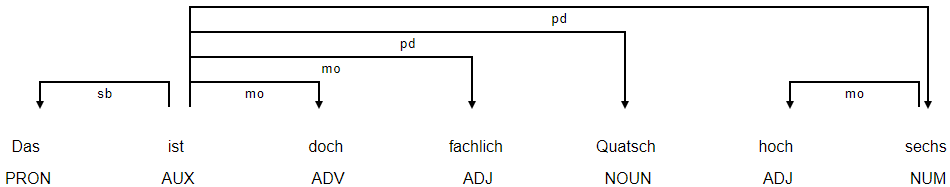
\includegraphics[width=1\textwidth]{chapters/04-Sentiment-Analyse/steffi.png}}
\caption{Visualisierung der Wortabhängigkeiten (Zitat von Steffi Lemke MdB, 208. Sitzung, 10.02.2021)}
\label{steffi}
\end{figure}

\subsection{Negations-Erkennung}
\label{neg-erkennung}
Negation, also Ablehnung, Verneinung oder Aufhebung, hat einen erheblichen Einfluss auf das Ergebnis und damit die Korrektheit der Sentimentanalyse, weshalb in dieser Arbeit ein besonderes Augenmerk auf ihre Erkennung gelegt wurde. 
In \textit{Negation Modeling for German Polarity Classification} \cite{g3_wieg} präsentieren Forscher der Universität des Saarlandes und des Leibniz-Institut für Deutsche Sprache hierfür einen regelbasierten Ansatz. 

Sie definieren unterschiedliche Negationstypen und ihre jeweilige Reichweite. 
So beeinflussen etwa negierende Adverbien oder Indefinitpronomen wie \textit{nie} den gesamten Satz, wohingegen das Partikel \textit{nicht} lediglich seinen Vorgänger negiert.  
Die Tabelle \ref{g3tab1} führt alle in dieser Arbeit implementierten Negationsregeln auf. 
Die Nutzung eines Abhängigkeitsbaumes, wie von \mintinline{latex}{spaCy} ermittelt, ist dabei unerlässlich. 
Denn wie schon im vorherigen Kapitel angesprochen, ist etwa mit dem Vorgänger eines Wortes nicht das in der Satzabfolge voranstehende Wort gemeint, sondern vielmehr der semantische Regent. 

\begin{table}[htbp]
\caption{Implementierte Negations-Regeln aus \cite{g3_wieg}}
\begin{center}
\begin{tabular}{| c | c | c |}
\hline
\textbf{Negationstyp} & \textbf{Reichweite} & \textbf{Beispielworte} \\ \hline
Partikel & Vorgänger (Regent) & nicht \\ \hline
Präpositionen & Nachfolger (Dependent) & ohne, gegen \\ \hline
Adverbien, & Satz & nie, kein, kaum \\
Indefinitpronomen &  &  \\ \hline
Nomen & Genitiv,& Abschaffung, \\
 & Präpositionalobjekt & Zerstörung \\ \hline
Verben & Objekt, Subjekt & enden, sinken, lindern \\
\hline
\end{tabular}
\label{g3tab1}
\end{center}
\end{table}

Angemerkt sei an dieser Stelle, dass es nicht möglich war, alle Regeln aus \cite{g3_wieg} zu implementieren, da der von den Forschern genutzte Dependency-Parser umfangreichere Ergebnisse liefert, als jener von \mintinline{latex}{spaCy}. 

Eine Liste mit Negationsworten und dem jeweiligen Negationstyp wurde \cite{g3_polcla} entnommen und ist ebenfalls über die Klasse \mintinline{latex}{Lexicon} zugreifbar. 
Die Klasse stellt ein \mintinline{latex}{Dictionary} bereit, in welchem die Schlüssel die Negationsworte und die Werte eine Liste der Reichweiten sind. 

Wenn in einem Text ein Negationswort auftritt, werden alle implementierten Regeln geprüft. 
Sollte es zu einem Treffer kommen, etwa wenn das Wort \textit{nicht} auftritt (siehe Abb. \ref{brandner}) und es einen Vorgänger gibt, werden alle Worte in Reichweite des Negationswortes negiert. 
Dies geschieht, indem für die jeweiligen Worte, welche wie in \ref{g3textv} beschrieben \mintinline{latex}{Token}-Objekte sind, ein eigenes Attribut mit der Bezeichnung \mintinline{latex}{negated} auf \mintinline{latex}{True} gesetzt wird. 
In der Polaritätsberechnung wird wortweise auf dieses Attribut geprüft und die Wort-Polarität bei einer Negierung mit -1 multipliziert. 

\begin{figure}[htb]
\centerline{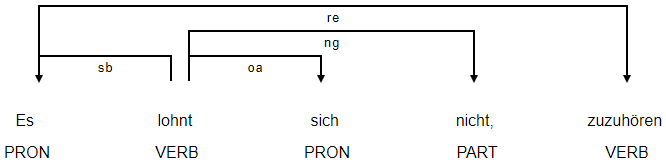
\includegraphics[width=1\textwidth]{chapters/04-Sentiment-Analyse/brandner.png}}
\caption{Beispielsatz mit Patikel-Negation (Zitat von Stephan Brandner MdB, 207. Sitzung, 29.01.2021)}
\label{brandner}
\end{figure}

\subsection{Verstärkungs-Erkennung}
\label{ver-erkennung}
Als \textit{Verstärker} werden sog. Gradpartikel (z.B. sehr, besonders, viel) verstanden, welche direkt vor Adjektiven oder Adverbien in einem Satz auftreten. 
Sie verstärken ihren Nachfolger, was wiederum in der Polaritätsberechnung berücksichtigt werden soll. 

Aus diesem Grund wird eine Liste mit verstärkenden Gradpartikeln, welche ebenfalls aus \cite{g3_polcla} bezogen werden, eingelesen und über die \mintinline{latex}{Lexicon} Klasse bereitgestellt. 

Ebenso wie in Kapitel \ref{neg-erkennung} bereits für die Negation beschrieben, wird ein eigenes Attribut zur Signalisierung einer Verstärkung definiert und im entsprechenden Fall auf True gesetzt. 
Bei der Polaritätsberechnung wird bei einer erkannten Verstärkung die Wort-Polarität mit 1,5 multipliziert \cite{g3_sentia}. 

In Abbildung \ref{hessel} wird ein Beispiel für das Auftreten eines verstärkenden Gradpartikels gegeben. 
Hier verstärkt das Wort \textit{sehr} das negative Wort \textit{spät}, womit die errechnete Polarität stärker negativ ausfällt als ohne die Verstärkungs-Erkennung. 

\begin{figure}[htb]
\centerline{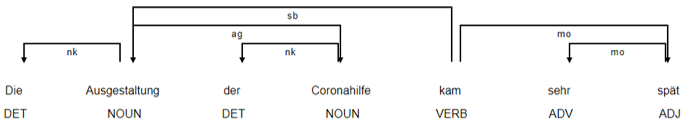
\includegraphics[width=1\textwidth]{chapters/04-Sentiment-Analyse/hessel.png}}
\caption{Beispielsatz mit Gradpartikel-Verstärkung (Zitat von Katja Hessel MdB, 206. Sitzung, 28.01.2021)}
\label{hessel}
\end{figure}

\subsection{Polaritätsberechnung}
\label{polberechnung}
Für die abschließende Berechnung der Polarität sind verschiedene Formeln denkbar. 
Sie sollten anhand von Textcharakteristika wie z.B. der Satz- oder Textlänge gewählt werden. 

Bei der Verwendung einer satzbasierten Polaritätsberechnung, bei welcher alle Polaritäten erst addiert und die Summe anschließend durch die Anzahl der Worte dividiert wird, kann ein unerwünschtes Phänomen auftreten: 
Längere Sätze erhaltenen ein stärker polarisiertes Ergebnis als vergleichbare kurze Sätze. 

Dies ist mit einer im Schnitt höheren Dichte an Worten mit Polaritäts-Wert in längeren Sätzen zu erklären. 
Um diesem Problem entgegen zu wirken, wurde in dieser Arbeit eine Min-Max-Skalierung (siehe Formeln 1 - 3) auf Dokumentebene implementiert \cite{g3_sentia}. 

Die Entscheidung, diese Normalisierung anhand der Länge des gesamten Textes durchzuführen, wurde aufgrund der Charakteristika der zu analysierenden Interaktionen getroffen. 
Denn diese bestehen zu einem überwiegenden Teil aus einem einzelnen Satz von jedoch sehr unterschiedlicher Länge. 

\begin{align}
p' &= \frac{ p + 1 }{ text.len + 1 } \text{ für p $>$ 0}\\
p' &= \frac{ p - 1 }{ text.len + 1 } \text{ für p $<$ 0}\\
p' &= p \text{ für p $=$ 0}
\end{align}

\section{Evaluierung}
\subsection{Sprache im Bundestag}
\label{sprachebundestag}
Während der Entwicklung dieser Arbeit und den regelmäßig angestellten Zwischentests wurde ersichtlich, dass sich die Sprache im Bundestag etwa von jener in sozialen Netzwerken oder Produktbewertungen unterschiedet. 
Ein Interaktionstext setzt sich sowohl aus einzelnen, langen und komplexe Sätze zusammen, als auch aus einzelnen Ausrufen wie \textit{\glqq eieiei!\grqq} zusammen. 

Aus diesem Grund wurde die in \ref{polberechnung} beschriebene Normalisierung verwendet, da herkömmliche Berechnungsformeln zunächst widersprüchliche Ergebnisse lieferten. 
Gleichzeitig verbesserte die manuelle Durchsicht der häufigsten 15.000 Worte und Anfertigung einer eigenen Bundestags-Wortliste das Ergebnis deutlich. 
Viele der regelmäßig in Bundestagssitzungen verwendeten Worte gehören zur \textit{Politik-Domäne} und treten deshalb nicht in den Quell-Wortlisten auf. 
Hier wird erwartet, dass eine noch umfangreichere Bundestags-Wortliste einen weiteren positiven Einfluss auf das Endergebnis hätte. 
Aus Zeit- sowie Kompetenzgründen wurde diese Liste jedoch nicht erweitert. 

\subsection{Ironie und Sarkasmus}
Ebenso wie die im vorherigen besprochene \textit{Politiksprache}, treten auch Ironie und Sarkasmus vermehrt in den Sitzungen des Bundestages auf. 
Einfach umrissen, handelt es sich dabei um ein Stilmittel, bei dem das Gegenteil vom Gesagten gemeint ist. 
Sarkasmus ist dabei eine verstärkte Form der Ironie und kann auch als ein Angriff verstanden werden. 

Selbst für den menschlichen Leser ist allein am geschriebenen Text nicht immer ersichtlich, ob eine Aussage ironisch gemeint ist. 
Vielmehr wird für die richtige Deutung die Stimmlage, Gestik und Mimik der sprechenden Person benötigt. 

Ironie und Sarkasmus könne also erst recht nicht mit dem in dieser Arbeit verwendeten Wortlisten-Ansatz erkannt werden, womit ein unbekannter Teil der Interaktionen im Ergebnis die falsche Polarität besitzt. 
Gleichwohl gibt es Ansätze aus dem Bereich des maschinellen Lernens, welche dieses Problem behandeln. 
Jedoch setzen diese einen entsprechend annotierten Korpus vorraus und stammen zudem aus dem Bereich der sozialen Netzwerke, in welchen etwa mit \textit{Hashtags} die Ironie bereits vom Autor markiert wurde. 

\subsection{Fazit}
Trotzt der soeben beschriebenen Fehlerquellen, wurde dennoch ein gelungenes Ergebnis erzielt: 
Es wurde ein solider und erweiterbarer Algorithmus zur Sentimentananlyse von Texten geschaffen, welcher auf den bekanntesten Bibliotheken und Techniken der Textverarbeitung beruht. 
Dieser kann als Basis für weitere Anstrengungen bei der Sentimentanalyse von politischen Texten dienen. 

Eine Deutung der bisherigen Ergebnisse durch Politikwissenschaftler oder anderweitig in diesem Bereich kompetente Personen wird dabei empfohlen, um die beschriebenen Schwachstellen entsprechend zu behandeln oder neue zu identifizieren. 

Der Programmcode ist zudem vollständig und abgesichert in die Projektpipeline eingebunden. 
Er erweitert seine Ergebnis-Datenbank automatisch um neue Sitzungen und benachrichtigt anschließend nachfolgende Gruppen. 

\section{Grundlagen}\label{sec:07_02_grundlagen}
\section{Anforderungsanalyse und Konzept}\label{sec:08_03_anforderungen_konzept}


\section{Zusammenfassung und Ausblick}\label{sec:07_05_zusammenfassung}

\pagenumbering{roman}
\setcounter{page}{6}

\printbibliography[title={Literaturverzeichnis}]
\addcontentsline{toc}{chapter}{Literaturverzeichnis}
\newpage

\printglossaries
\addcontentsline{toc}{chapter}{Glossar}
\newpage

\end{document}